\section{Experimental Results}

\subsection{Tables of Most Significant Performance}
To manage the extensive dataset generated by this investigation, tables \ref{table:first_param_table} through \ref{table:last_param_table} present the score metrics for the best and worst performing HOG parameters, highlighting the top and bottom 10 configurations. Performance evaluation was conducted both at the individual dataset level and across the aggregate test sample, enabling analysis of parameter effectiveness at multiple scales. The tables for the performance scores of every parameter configuration are available in appendix \ref{appendix:tables_of_data}.

\subsubsection{Tables of Most Performant Parameters}\label{section:best_tables}

\begin{table}
    \centering
    \includegraphics[width=0.9\linewidth]{../tables/top10/INRIA_best_10.png}
    \caption{Top 10 performing HOG parameter configurations on the INRIA data set, ranked by MCC}
    \label{table:first_param_table}
\end{table}

\begin{table}
    \centering
    \includegraphics[width=0.9\linewidth]{../tables/top10/caltech_30_best_10.png}
    \caption{Top 10 performing HOG parameter configurations on the Caltech data set, ranked by MCC}
\end{table}

\begin{table}
    \centering
    \includegraphics[width=0.9\linewidth]{../tables/top10/PnPLO_best_10.png}
    \caption{Top 10 performing HOG parameter configurations on the PnPLO data set, ranked by MCC}
\end{table}

\begin{table}
    \centering
    \includegraphics[width=0.9\linewidth]{../tables/top10/total_best_10.png}
    \caption{Top 10 performing HOG parameter configurations on the aggregate test data set, ranked by MCC}
\end{table}

\subsubsection{Tables of Least Performant Parameters}\label{section:worst_tables}

\begin{table}
    \centering
    \includegraphics[width=0.9\linewidth]{../tables/top10/INRIA_worst_10.png}
    \caption{Bottom 10 performing HOG parameter configurations on the INRIA data set, ranked by MCC}
\end{table}

\begin{table}
    \centering
    \includegraphics[width=0.9\linewidth]{../tables/top10/caltech_30_worst_10.png}
    \caption{Bottom 10 performing HOG parameter configurations on the Caltech data set, ranked by MCC}
\end{table}

\begin{table}
    \centering
    \includegraphics[width=0.9\linewidth]{../tables/top10/PnPLO_worst_10.png}
    \caption{Bottom 10 performing HOG parameter configurations on the PnPLO data set, ranked by MCC}
\end{table}

\begin{table}
    \centering
    \includegraphics[width=0.9\linewidth]{../tables/top10/total_worst_10.png}
    \caption{Bottom 10 performing HOG parameter configurations on the aggregate test data set, ranked by MCC}
    \label{table:last_param_table}
\end{table}

\subsection{Graphical Presentation of Individual Parameter Influence}

While the table in sections \ref{section:best_tables} and \ref{section:worst_tables} clearly identify the set of parameters which should be used in real world applications, it would be wrong to extrapolate the overall performance impact of individual parameters from the tables alone. The graphs in this section group models into "sets", where each set contains models that differ only by a single, specified parameter. To better discern the trend of each individual graph, the MCC score values are uniformly filtered by taking the arithmetic average of each pixel with its neighbor (as implemented in scipy's \href{https://docs.scipy.org/doc/scipy/reference/generated/scipy.ndimage.uniform_filter1d.html}{uniform\_filter1d}). The highest MCC score for each set is highlighted with a marker.

\subsubsection{Graphs for Different Window Sizes}

\begin{figure}\
    \centering
    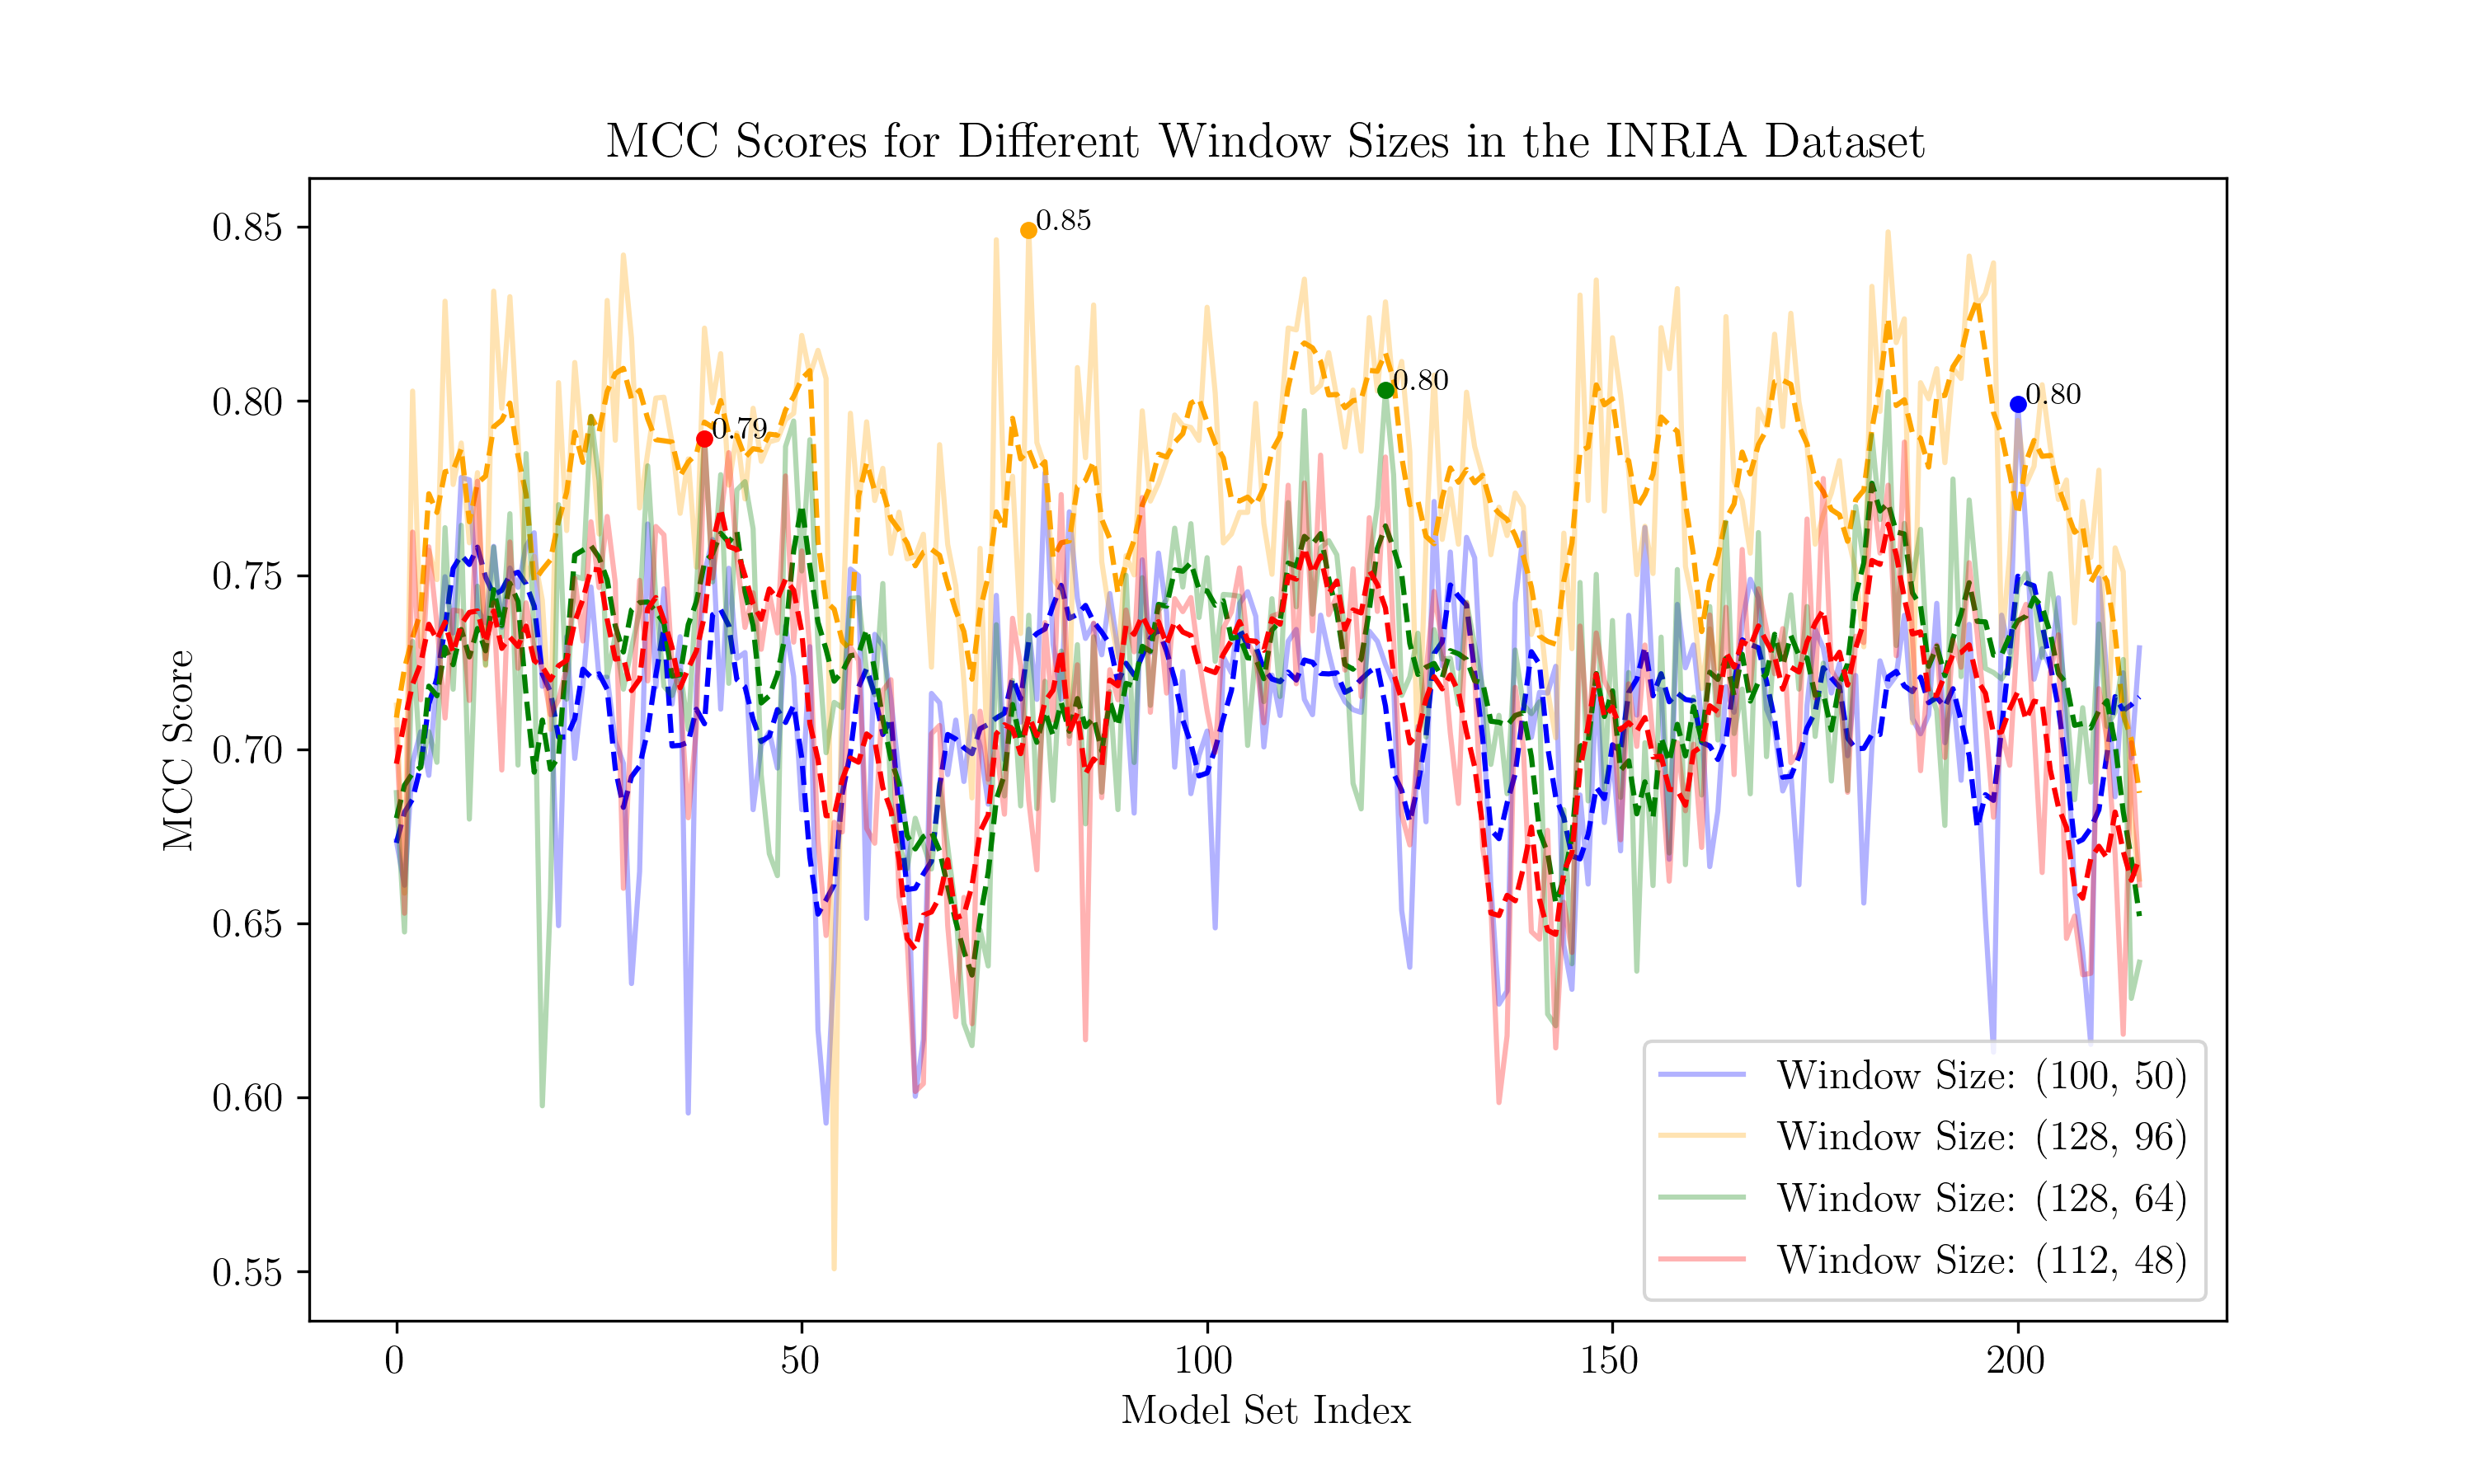
\includegraphics[width=0.9\linewidth]{../images/mcc_windows_INRIA.png}
    \caption{
        MCC scores for INRIA dataset, grouped by window size.
    }
    \label{fig:window_size_inria}
\end{figure}
\begin{figure}
    \centering
    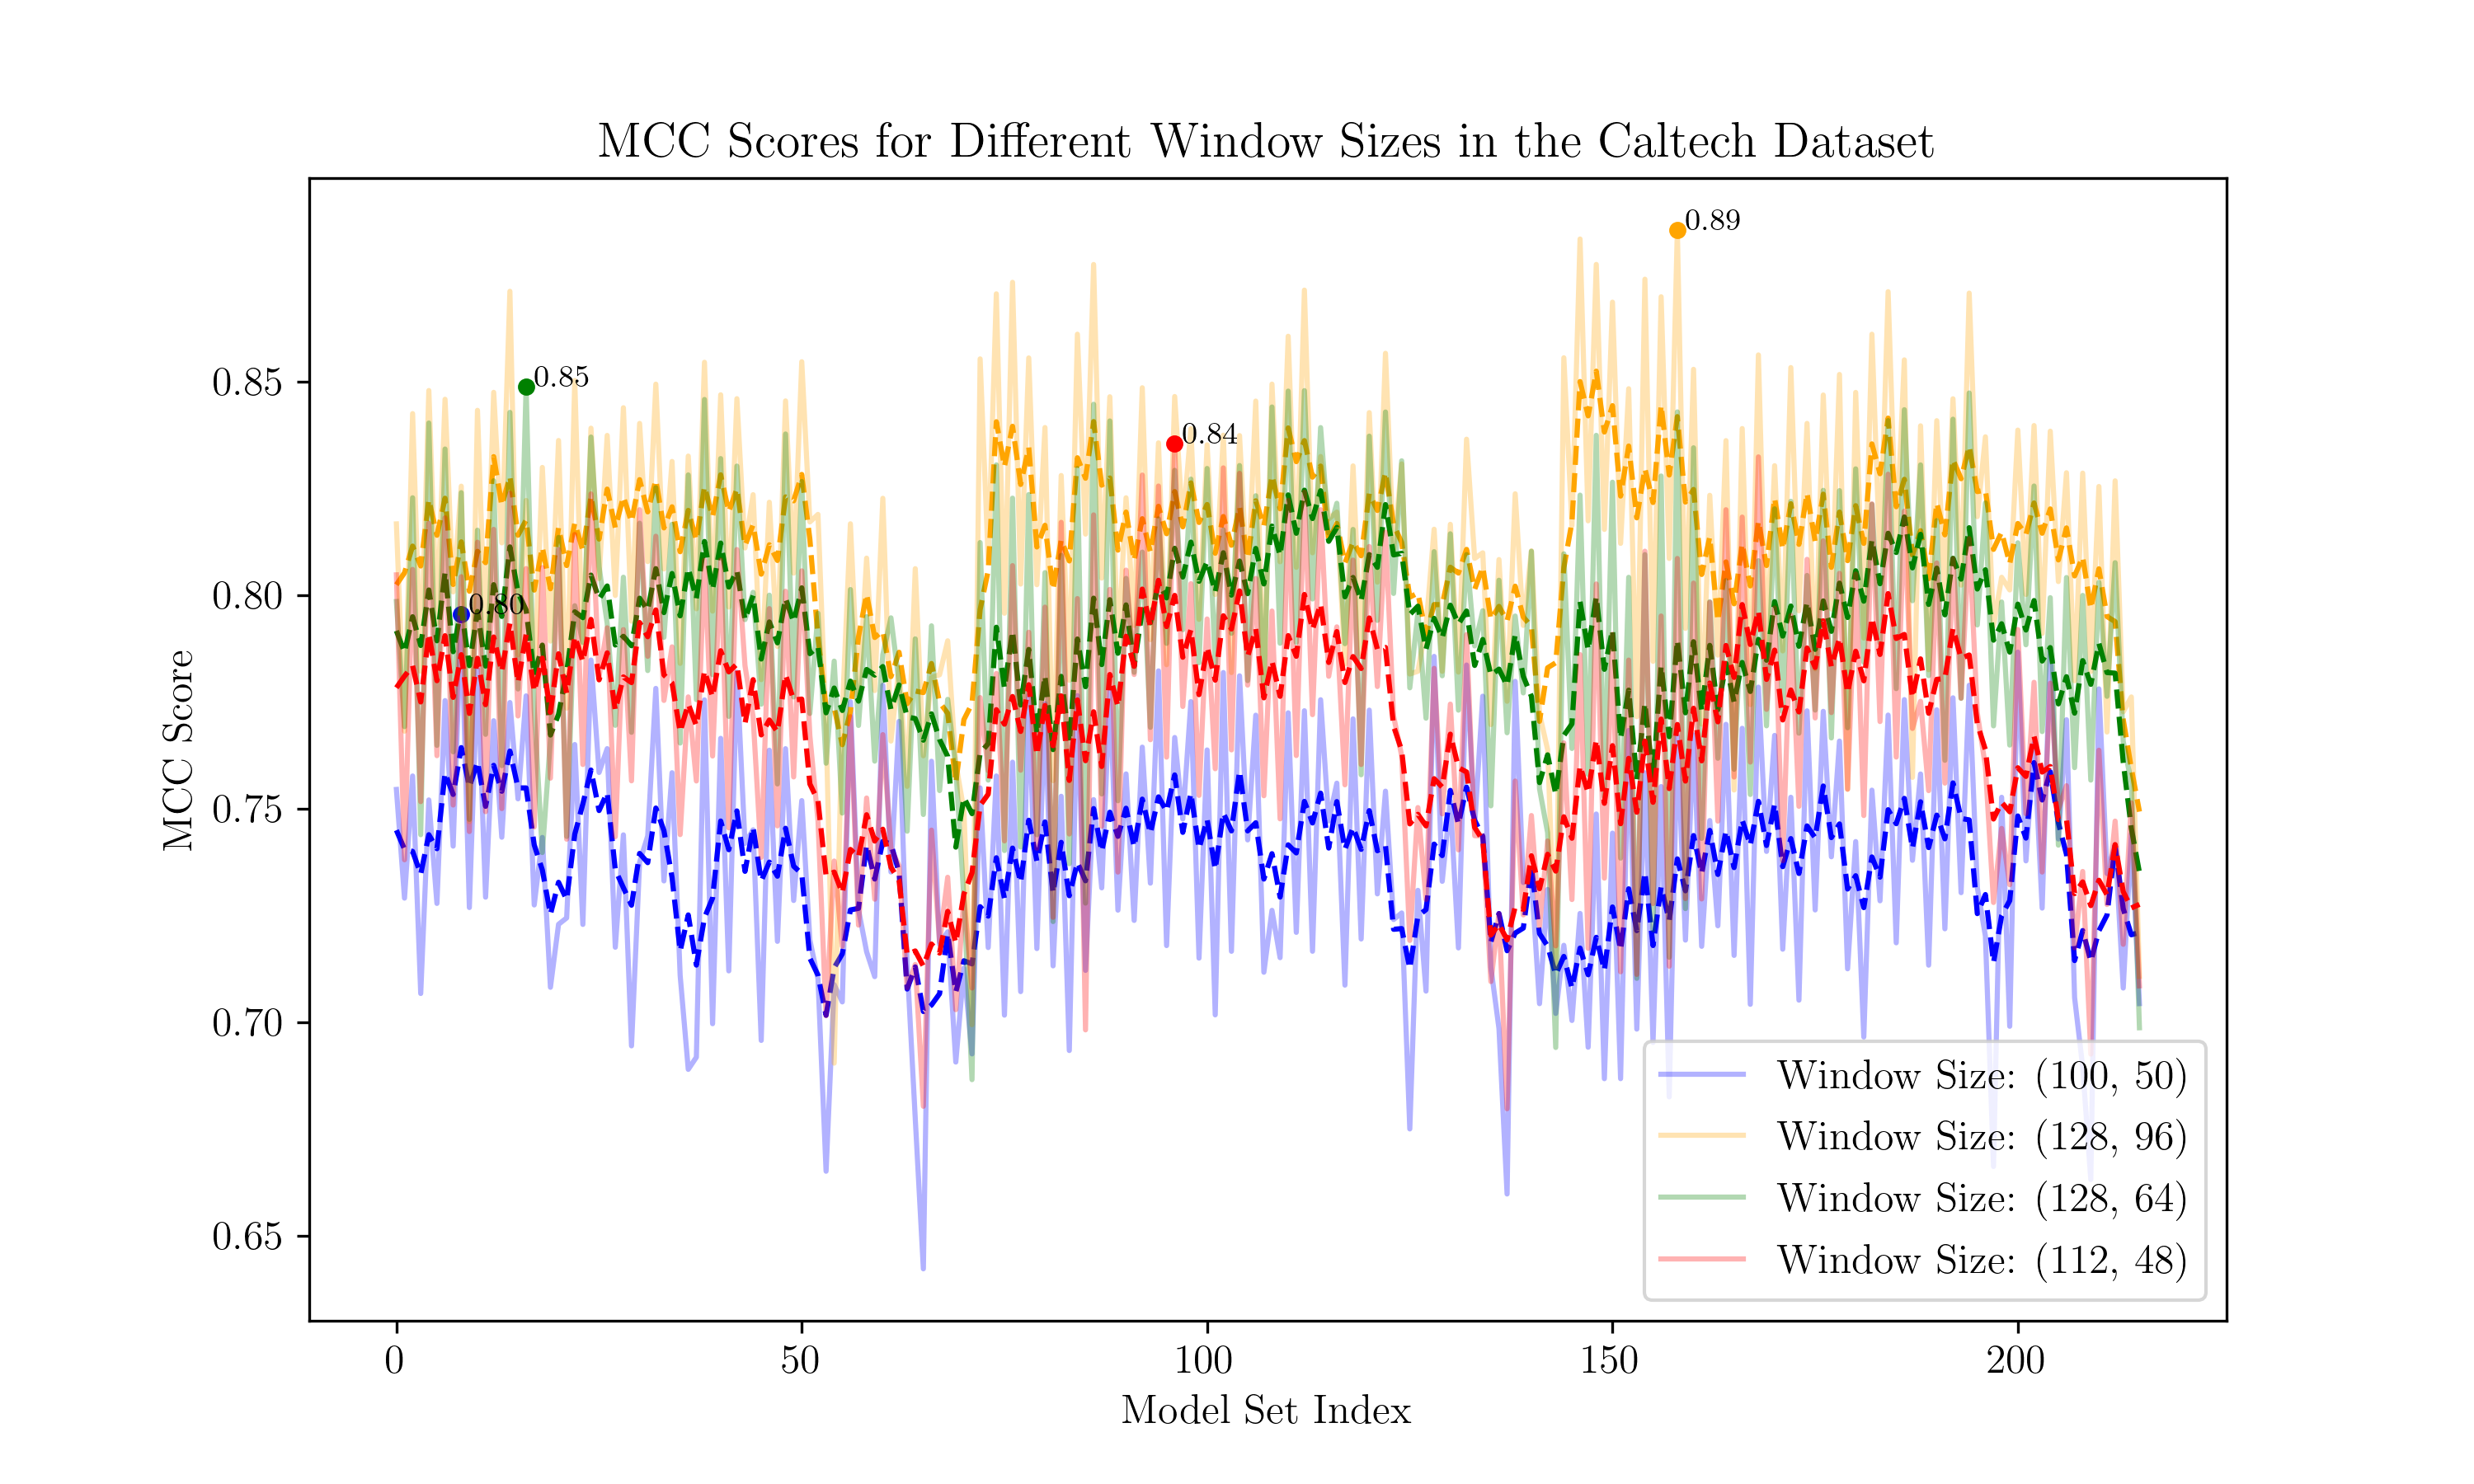
\includegraphics[width=0.9\linewidth]{../images/mcc_windows_caltech_30.png}
    \caption{
        MCC scores for Caltech dataset, grouped by window size.
    }
    \label{fig:window_size_caltech}

\end{figure}
\begin{figure}
    \centering
    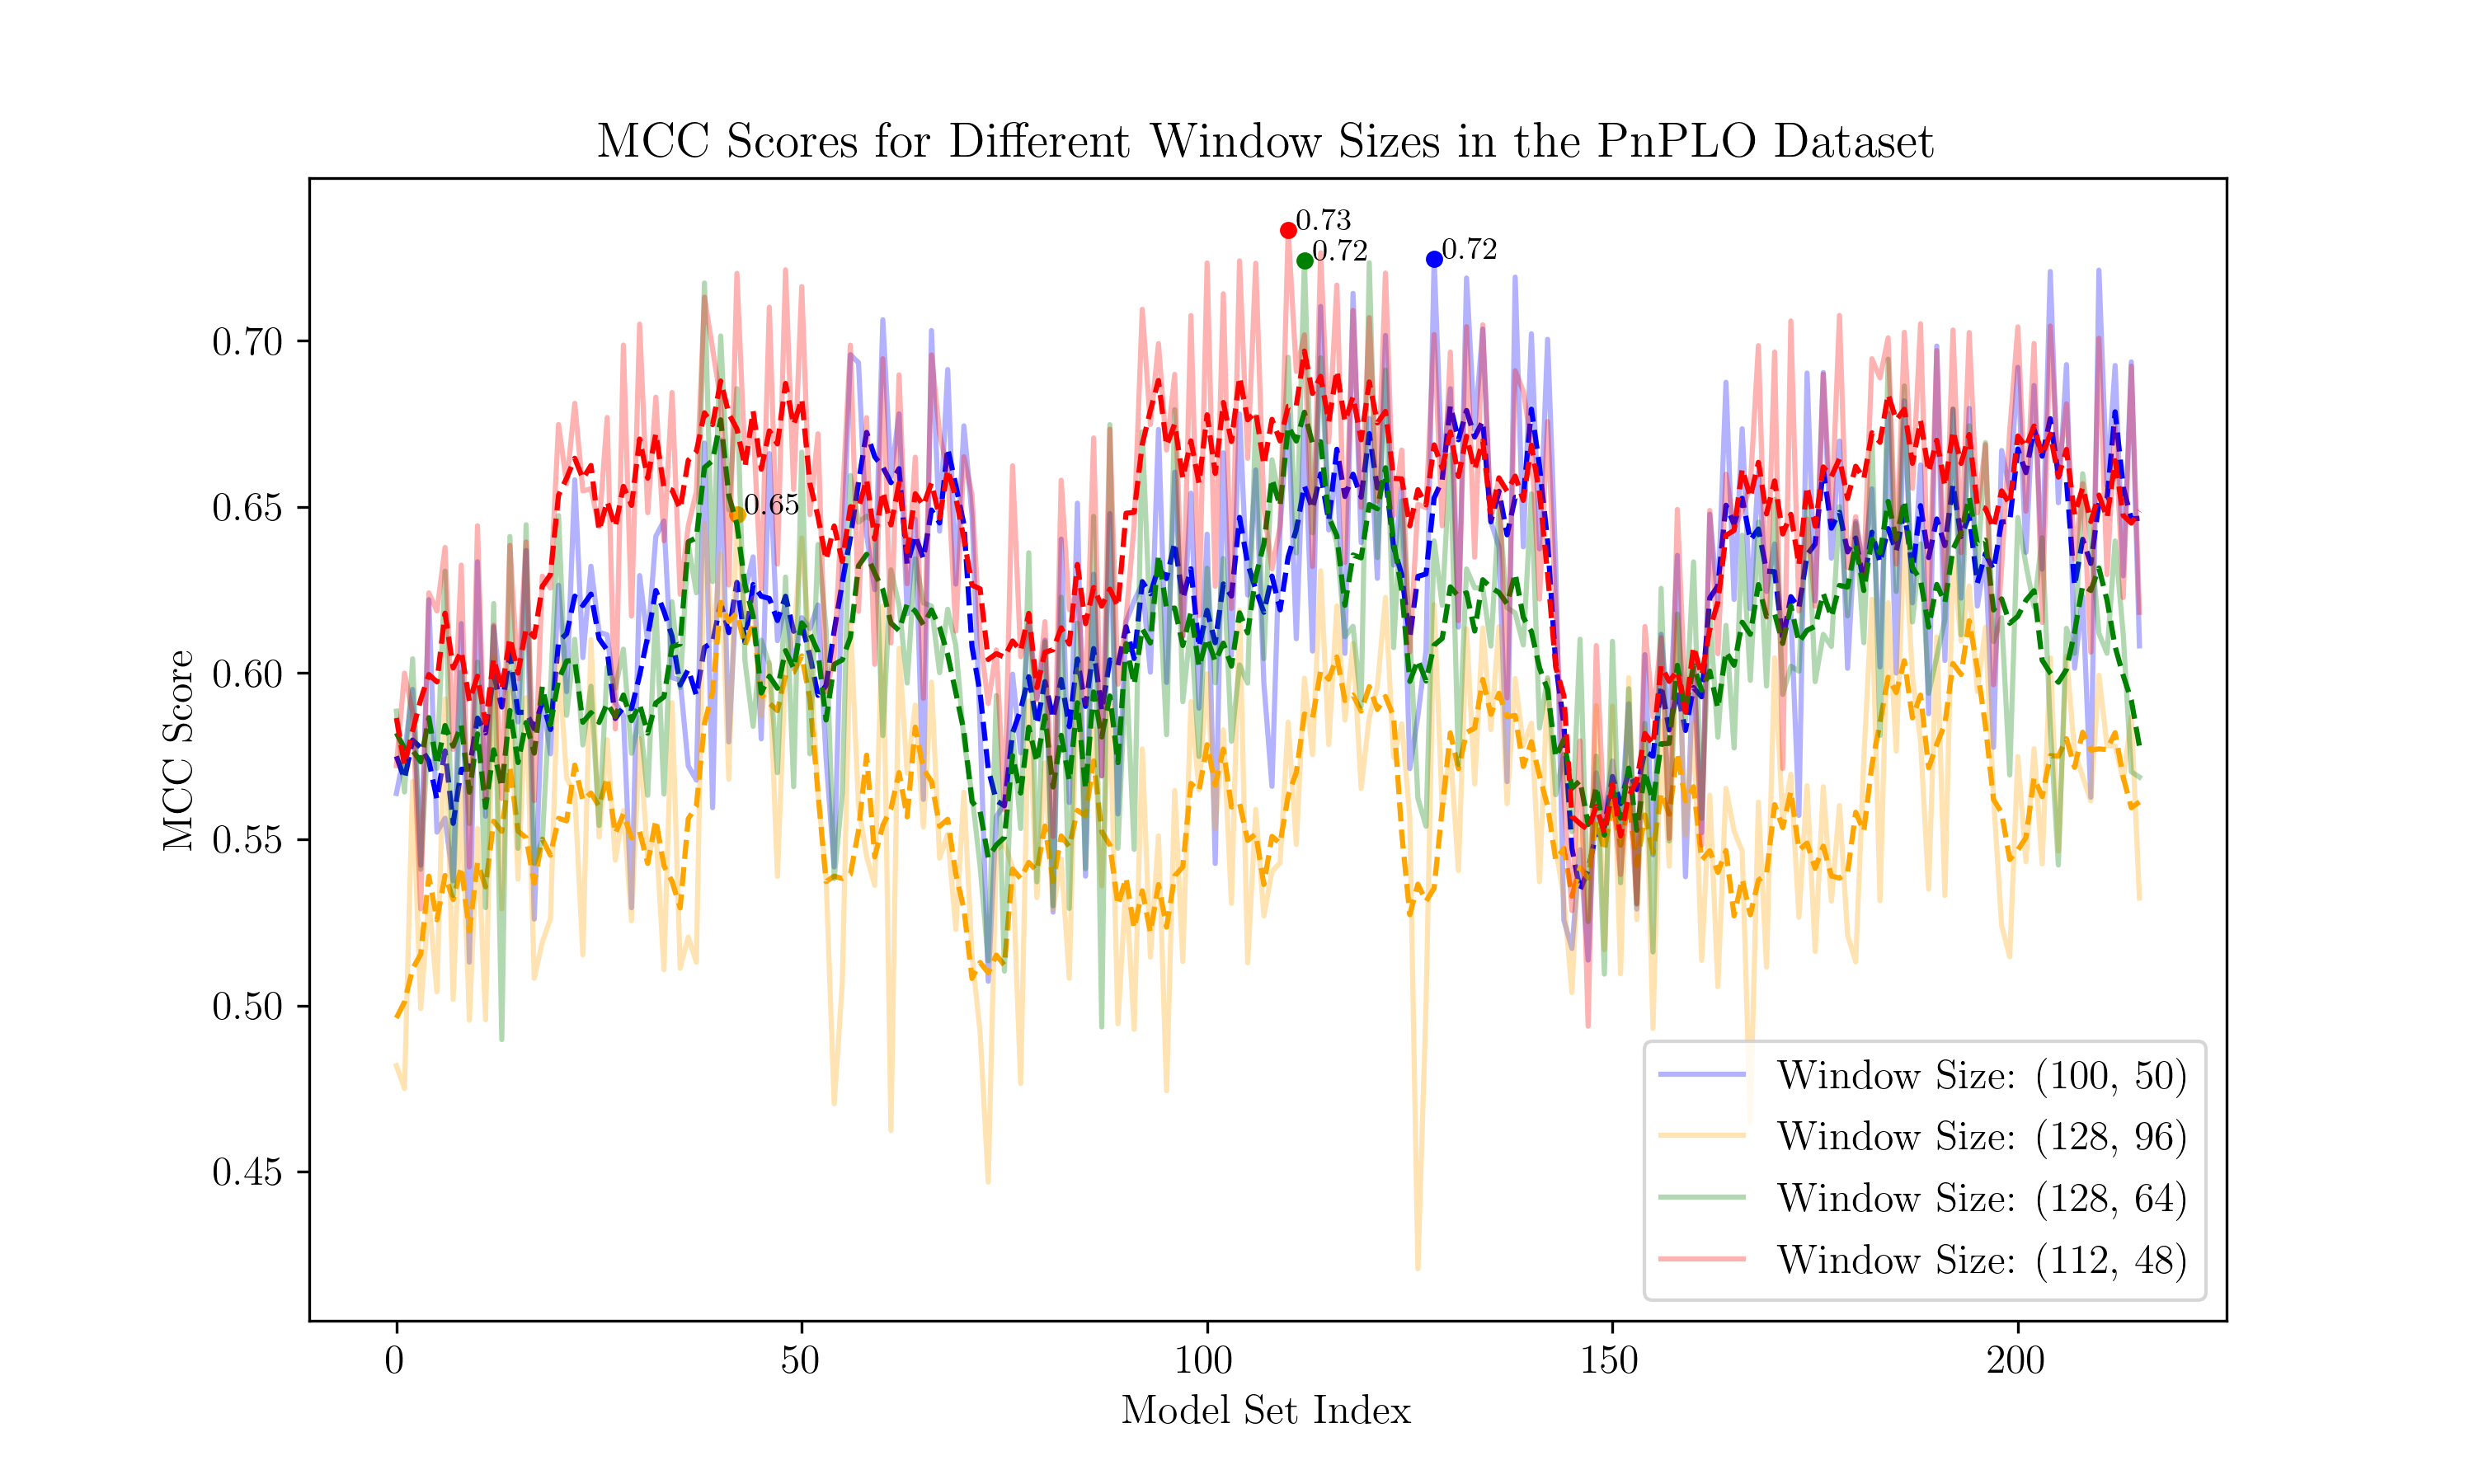
\includegraphics[width=0.9\linewidth]{../images/mcc_windows_PnPLO.png}
    \caption{
        MCC scores for PnPLO dataset, grouped by window size.
    }
    \label{fig:window_size_pnplo}
\end{figure}

\begin{figure}
    \centering
    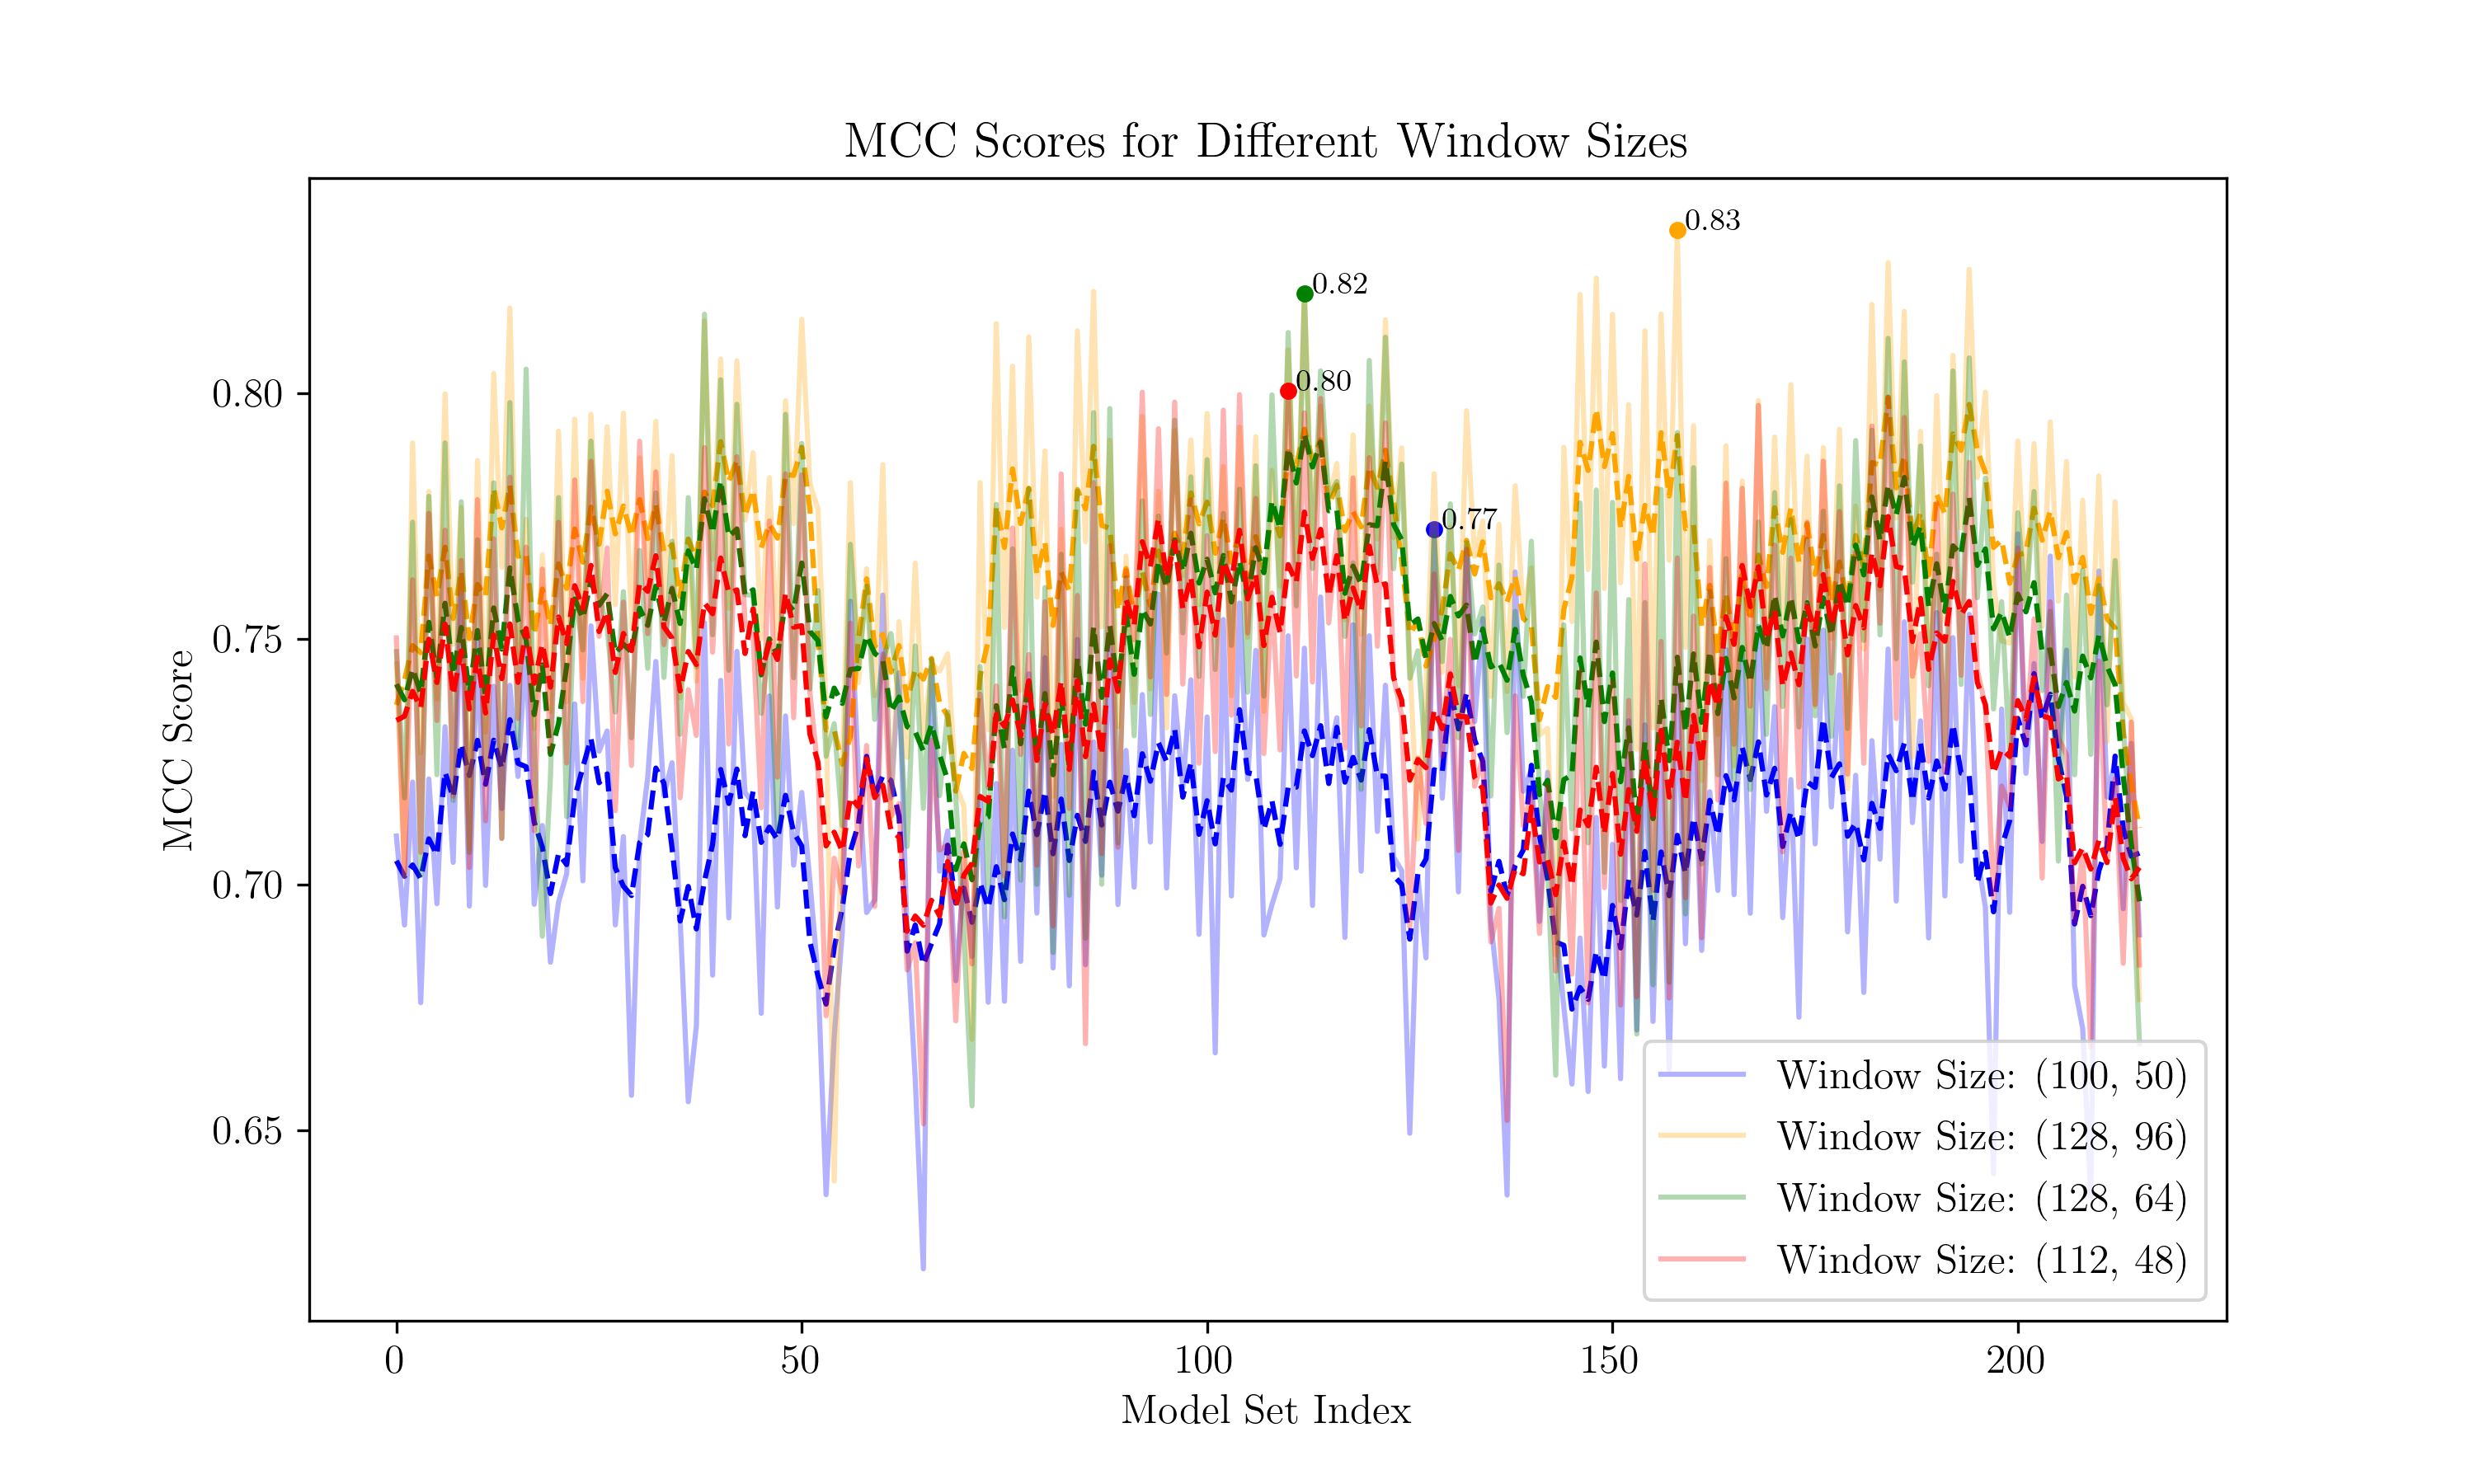
\includegraphics[width=0.9\linewidth]{../images/mcc_windows_total.png}
    \caption{
        MCC scores for the aggregate test dataset, grouped by window size.
    }
\end{figure}

\subsubsection{Graphs for Different Derivative Masks}


\begin{figure}
    \centering
    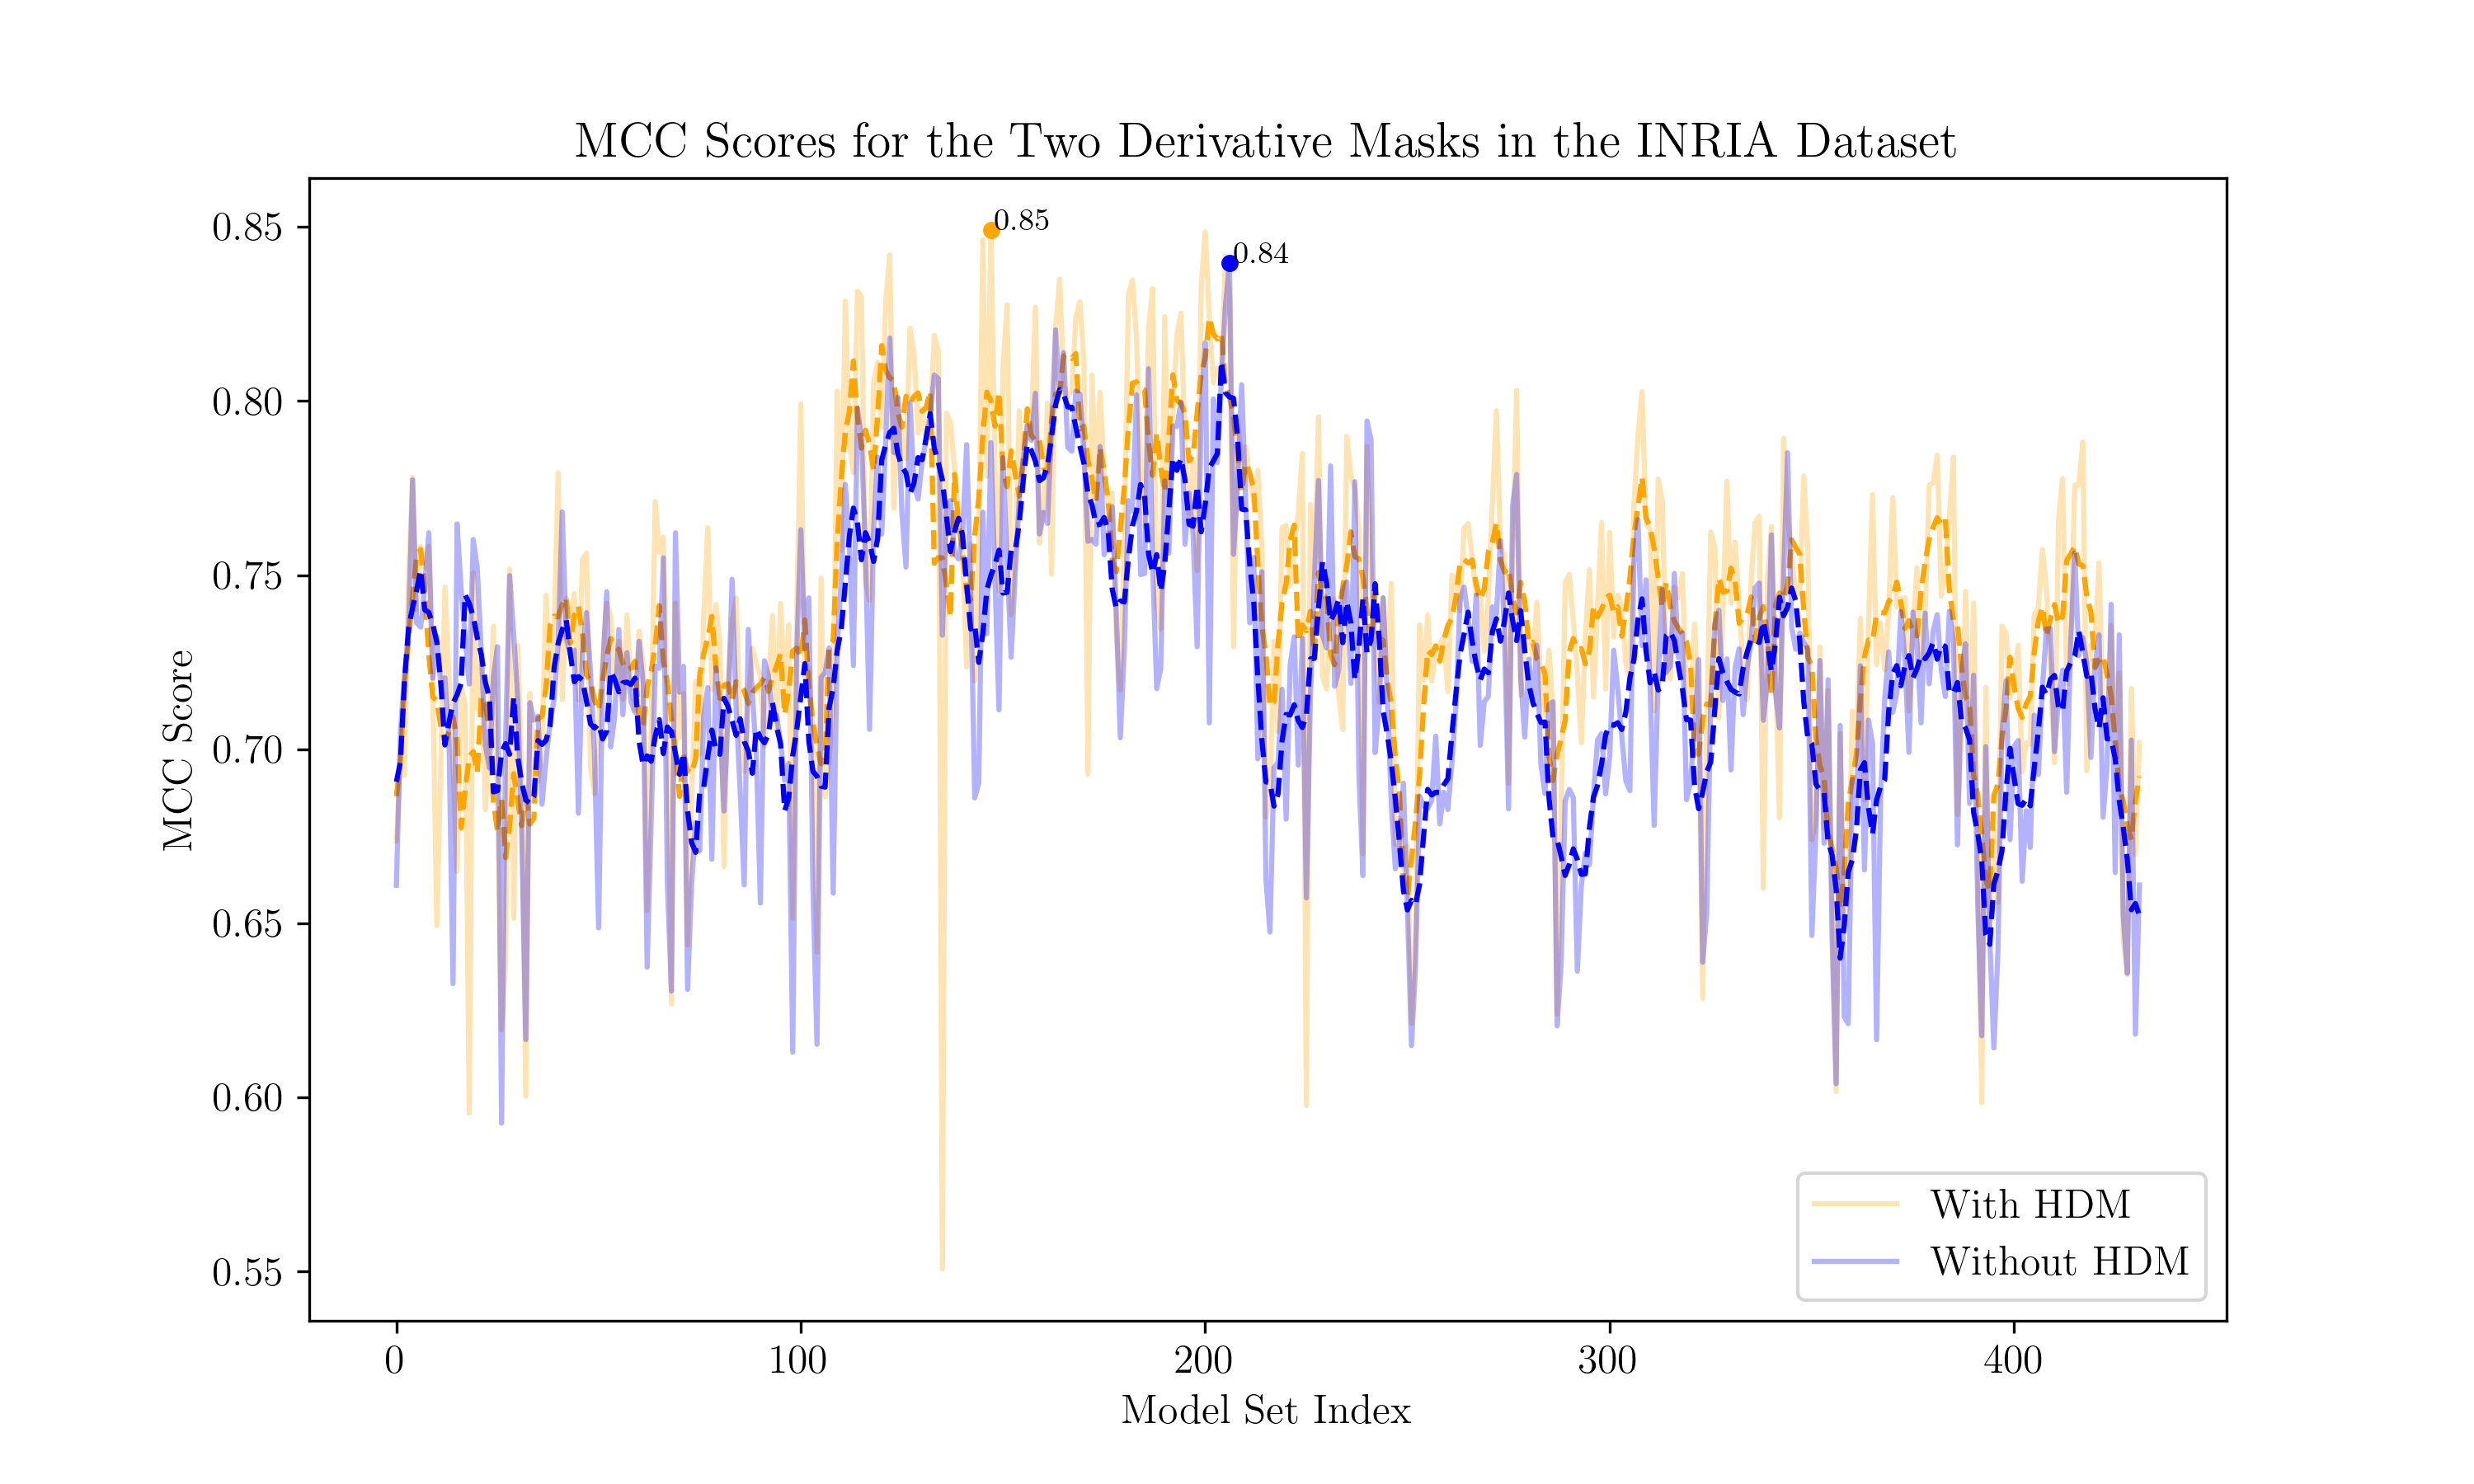
\includegraphics[width=0.9\linewidth]{mcc_hdm_INRIA.png}
    \caption{
        MCC scores for the INRIA dataset, grouped by derivative mask. HDM stands for holistic derivative mask, as introduced in section \ref{sec:deriv_mask}.
    }
    \label{fig:hdm_inria}
\end{figure}
\begin{figure}
    \centering
    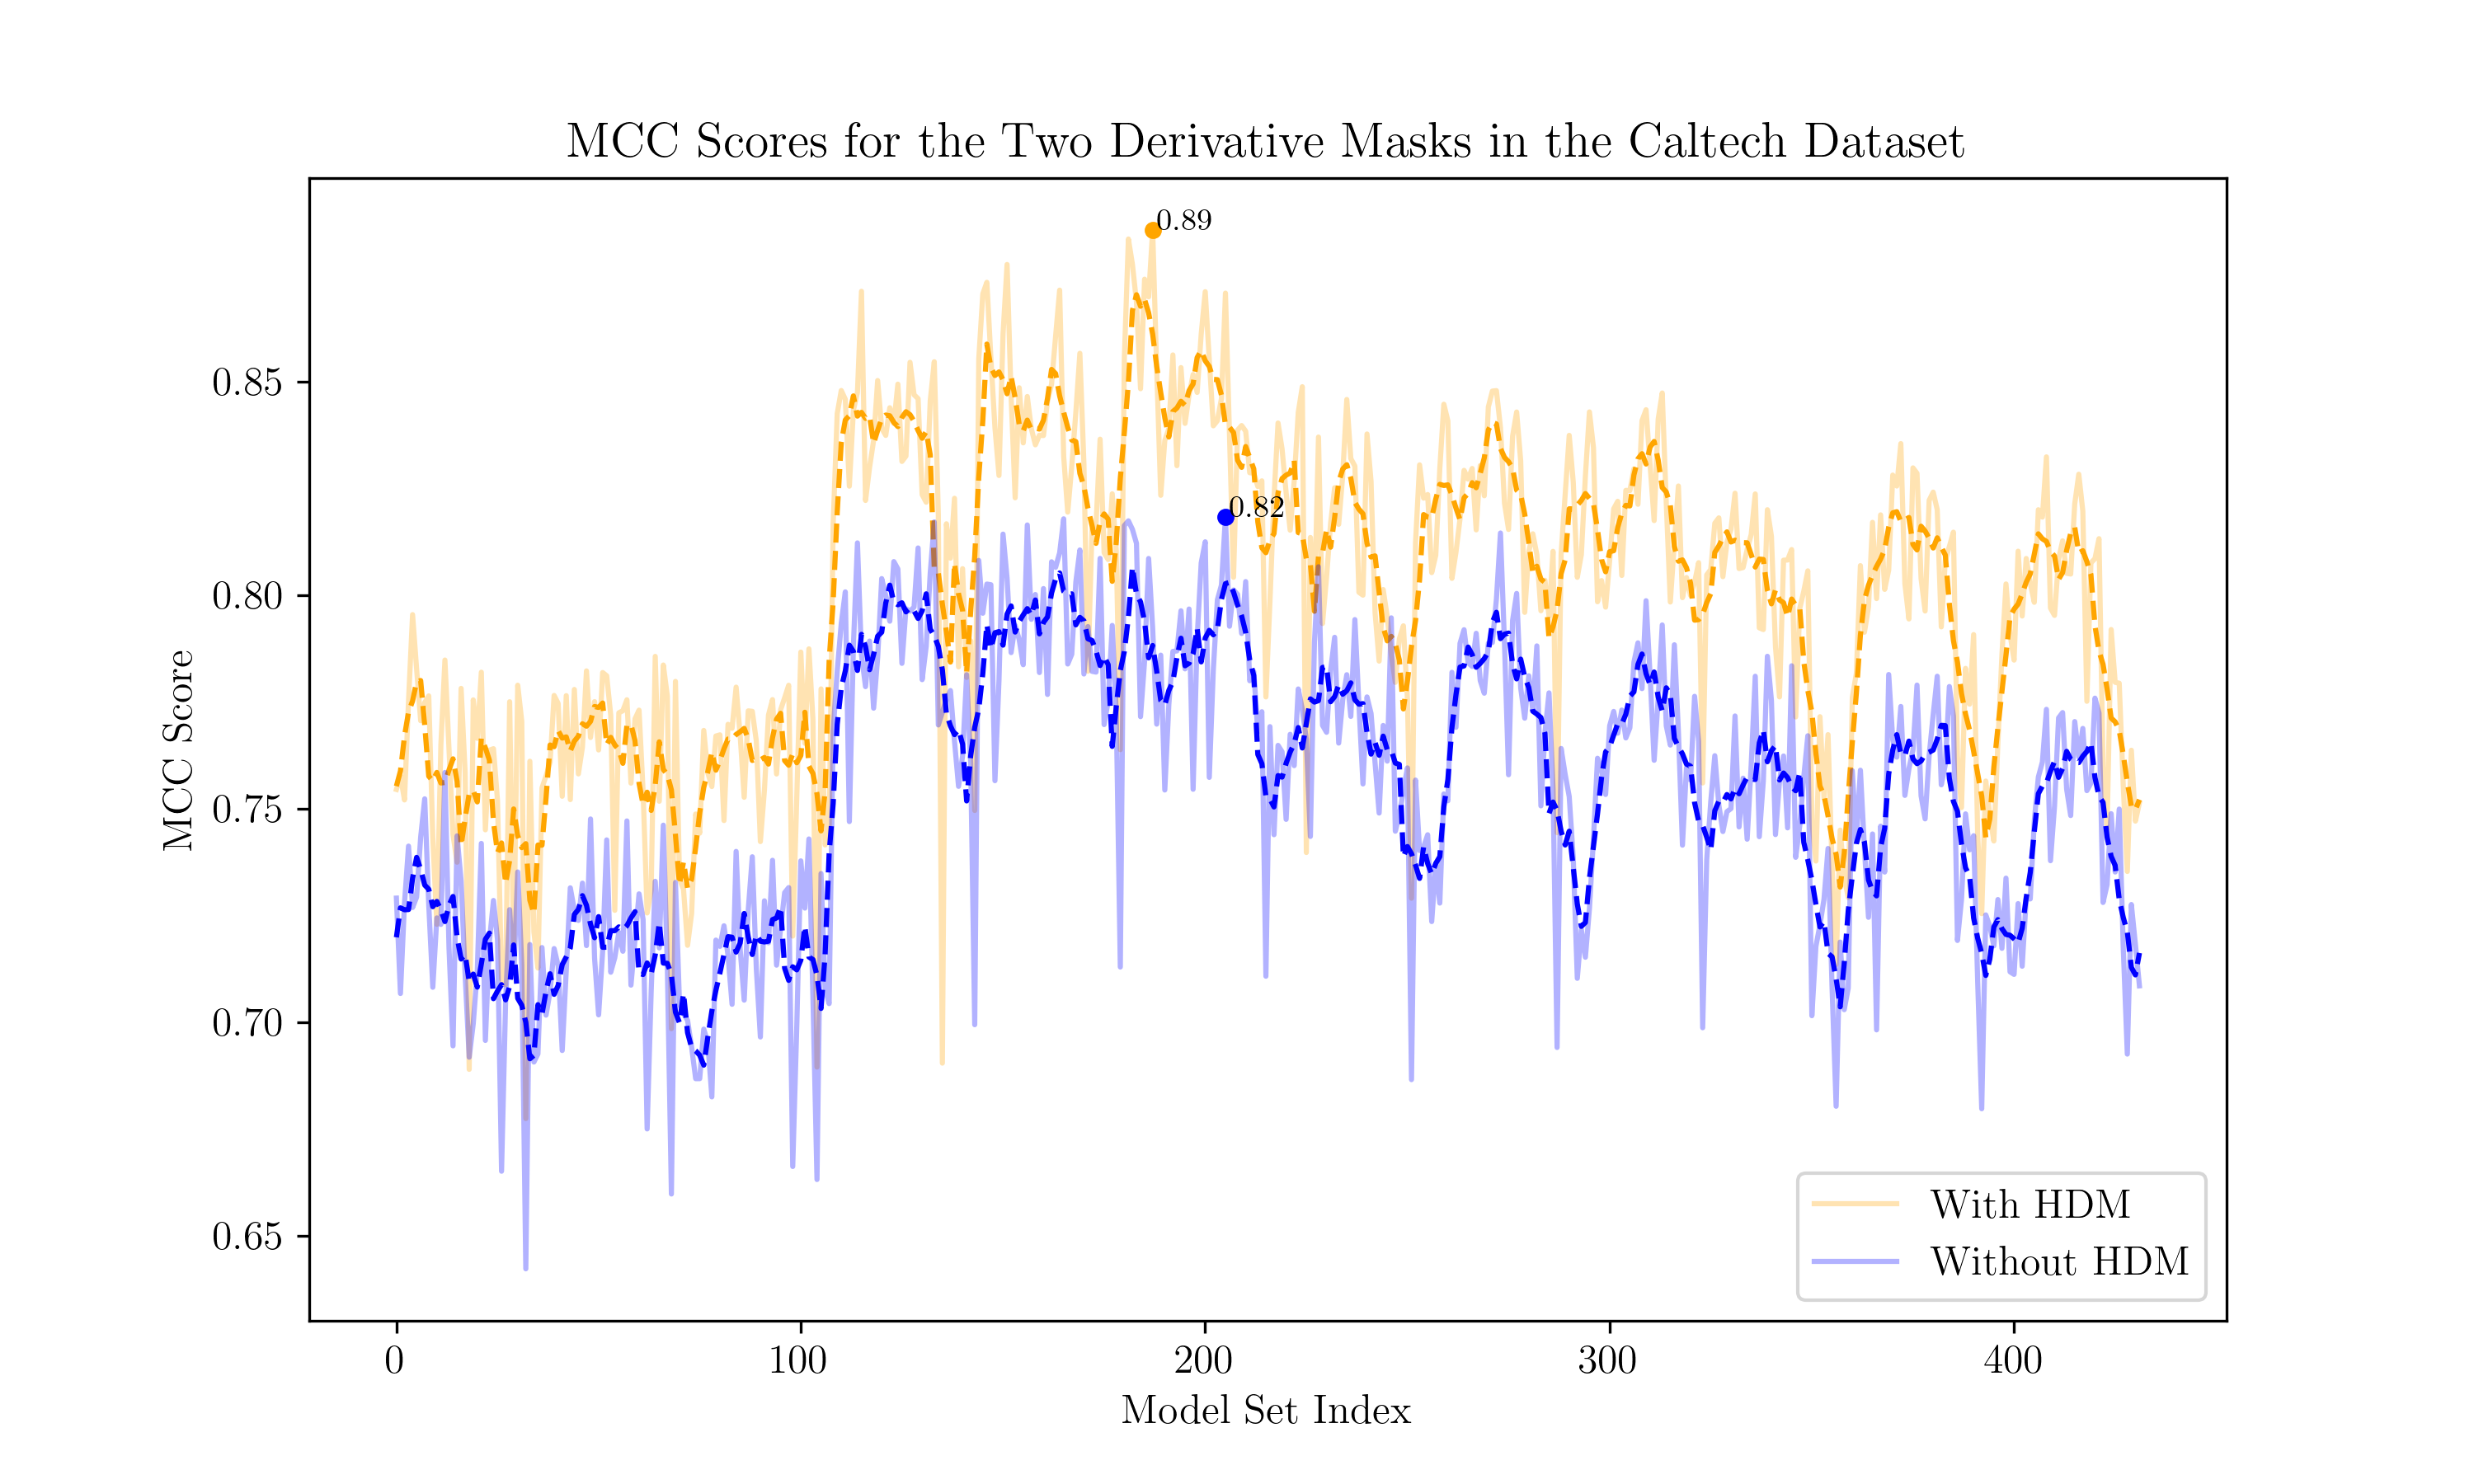
\includegraphics[width=0.9\linewidth]{mcc_hdm_caltech_30.png}
    \caption{
        MCC scores for Caltech dataset, grouped by derivative mask. HDM stands for holistic derivative mask, as introduced in section \ref{sec:deriv_mask}.
    }
    \label{fig:hdm_caltech}
\end{figure}
\begin{figure}
    \centering
    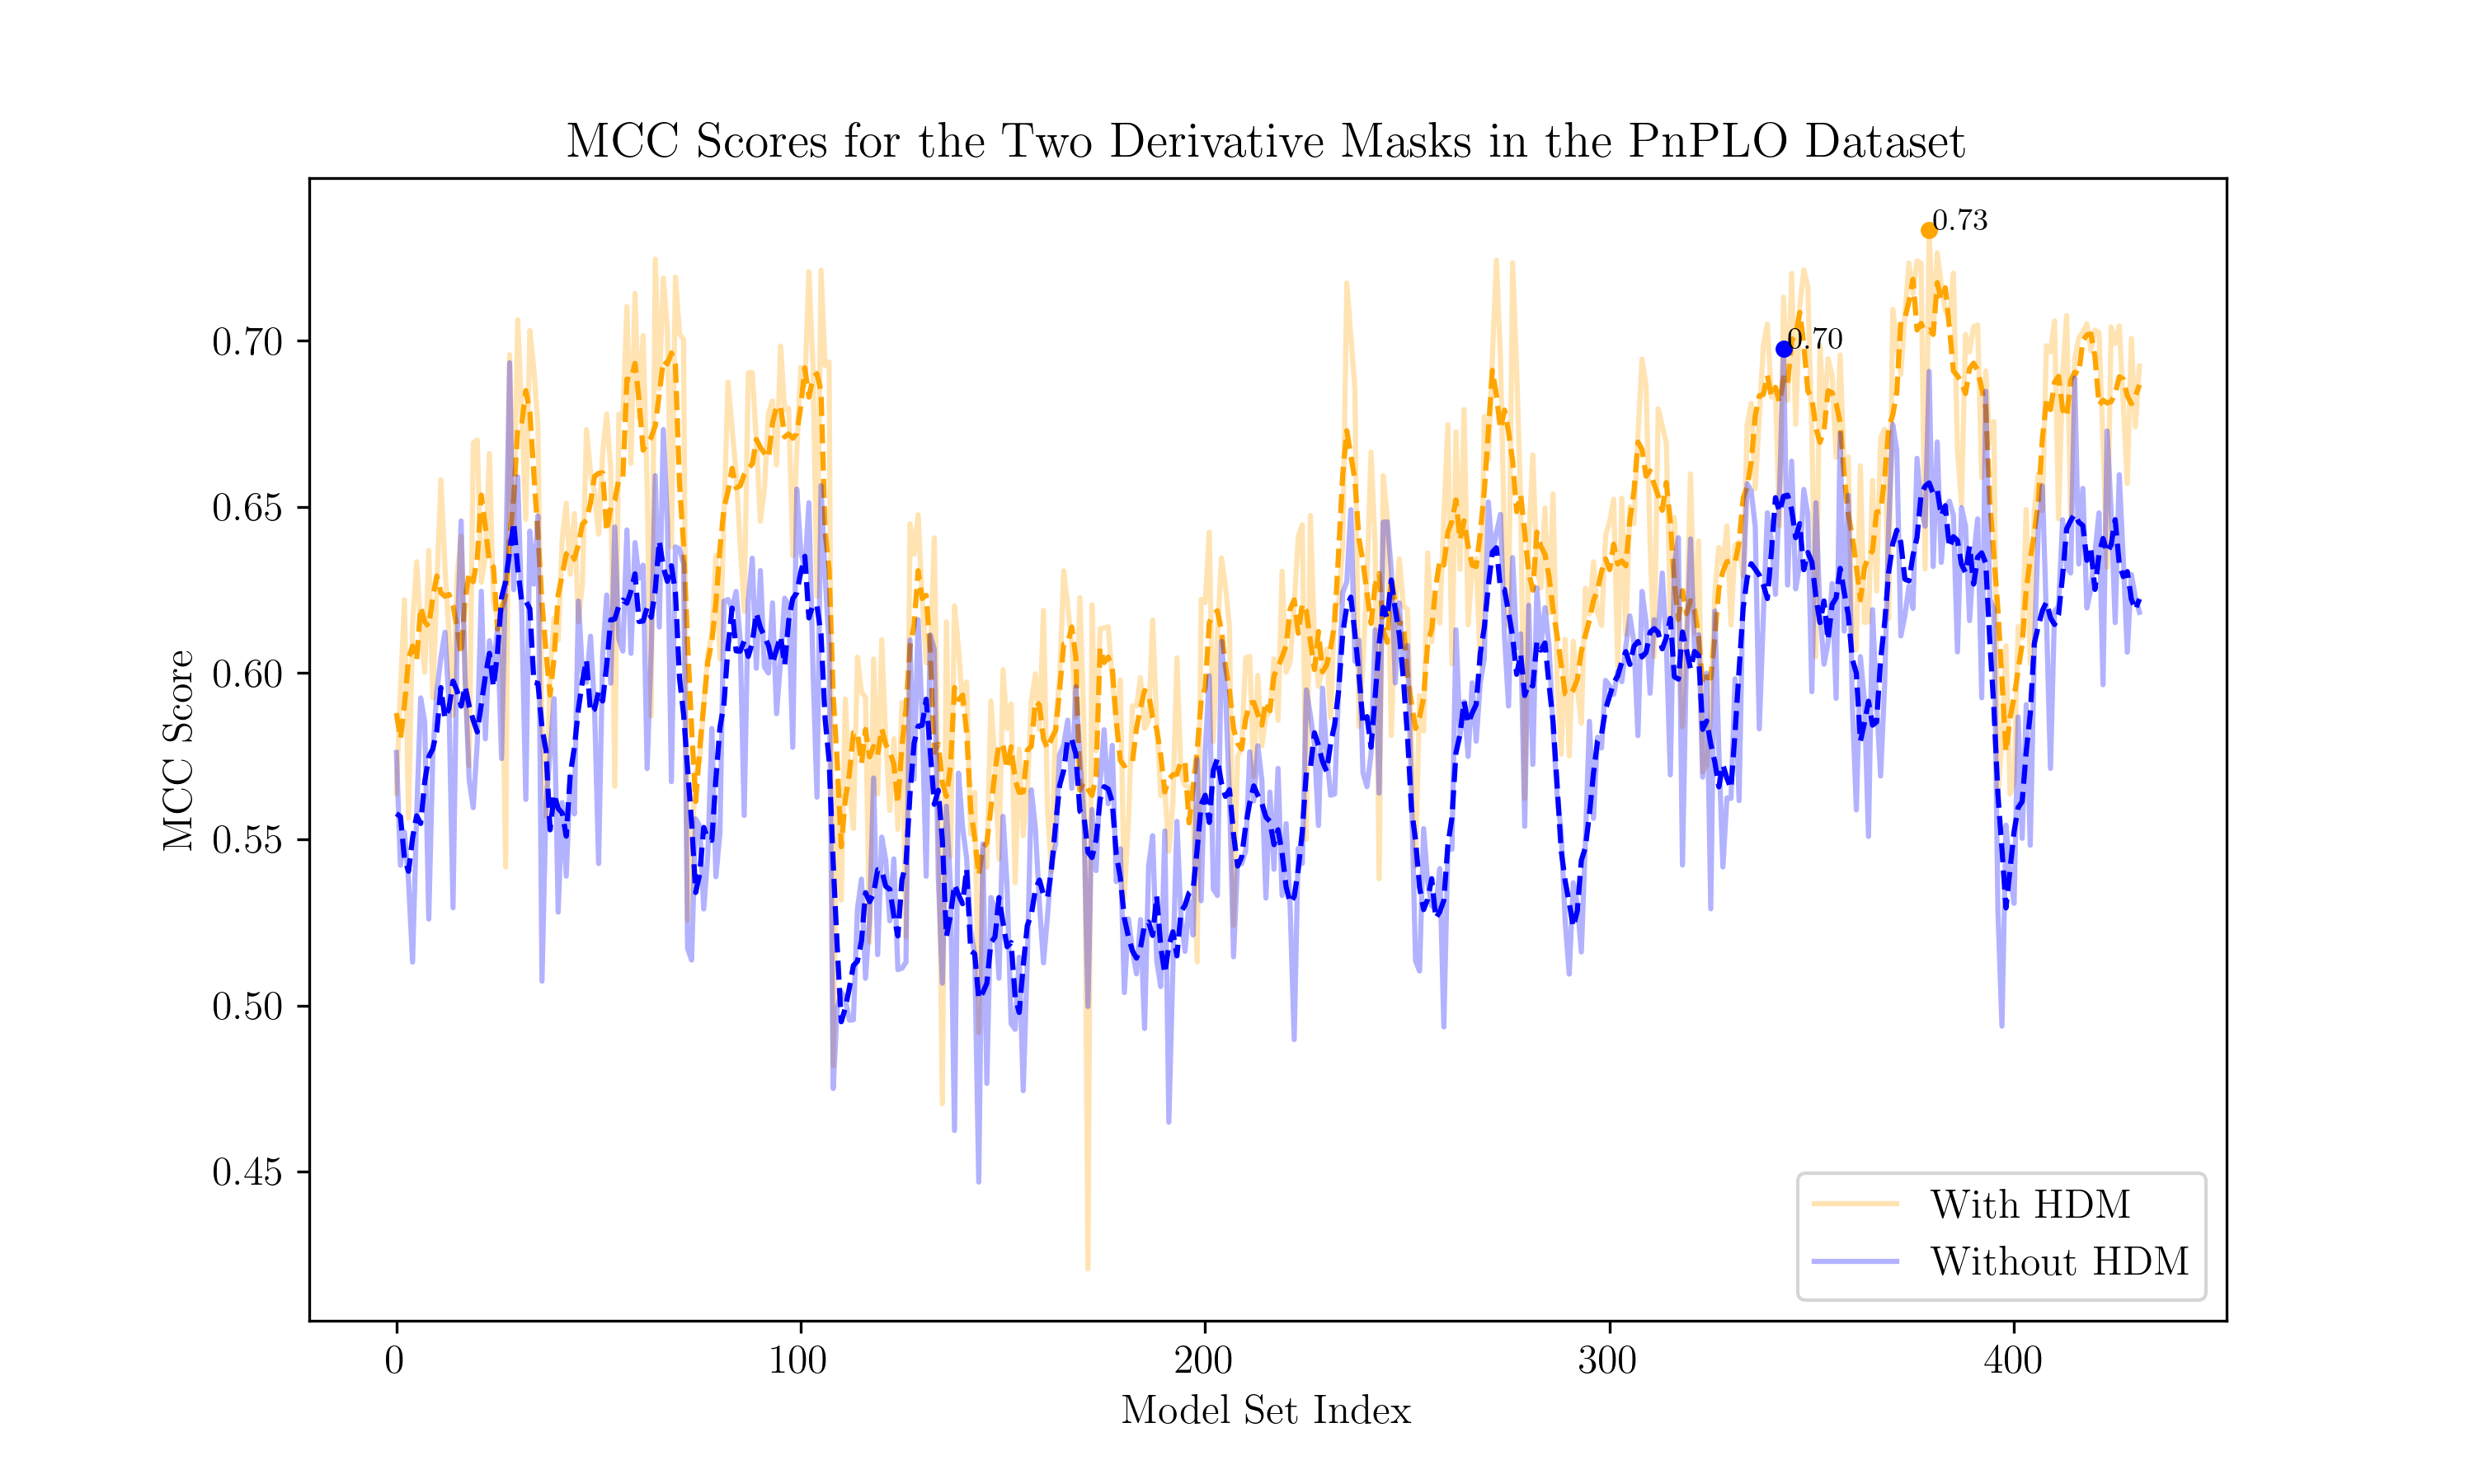
\includegraphics[width=0.9\linewidth]{mcc_hdm_PnPLO.png}
    \caption{
        MCC scores for PnPLO dataset, grouped by derivative mask. HDM stands for holistic derivative mask, as introduced in section \ref{sec:deriv_mask}.
    }
    \label{fig:hdm_pnplo}
\end{figure}

\begin{figure}
    \centering
    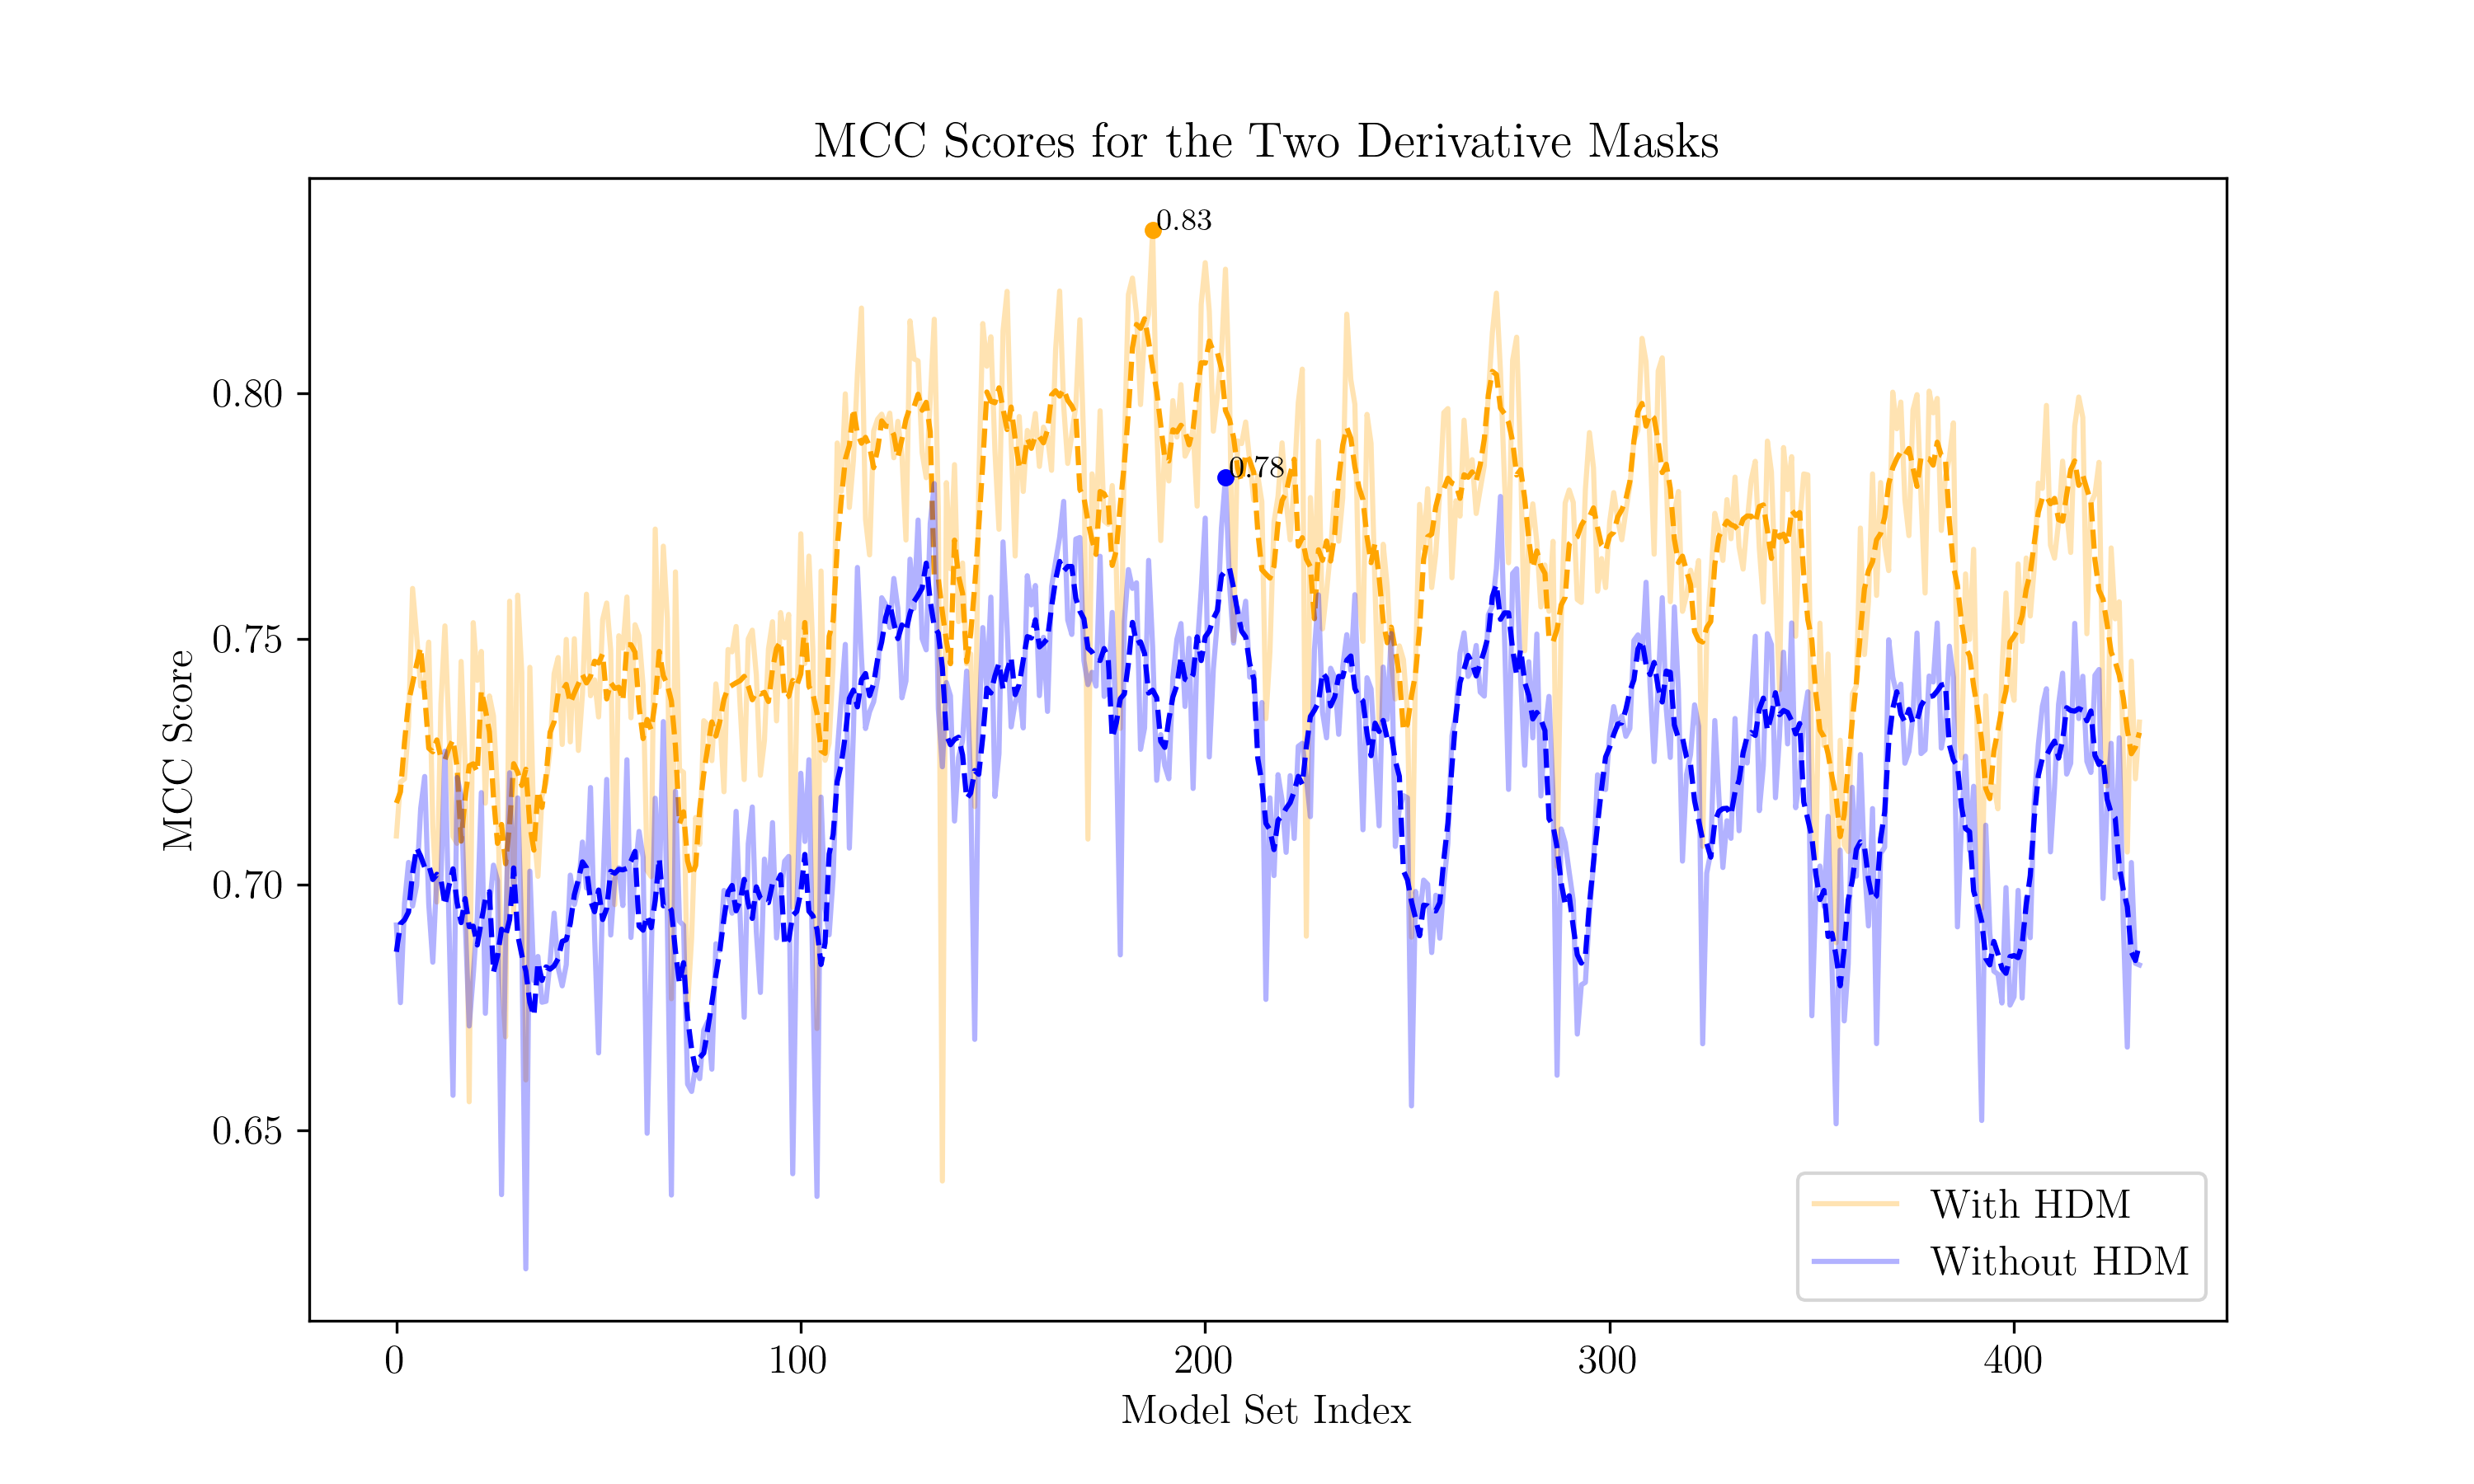
\includegraphics[width=0.9\linewidth]{mcc_hdm_total.png}
    \caption{
        MCC scores for the aggregate test dataset, grouped by derivative mask. HDM stands for holistic derivative mask, as introduced in section \ref{sec:deriv_mask}.
    }
    \label{fig:hdm_total}
\end{figure}


\subsubsection{Graphs for Different Orientation Bin Sizes}

\begin{figure}
    \centering
    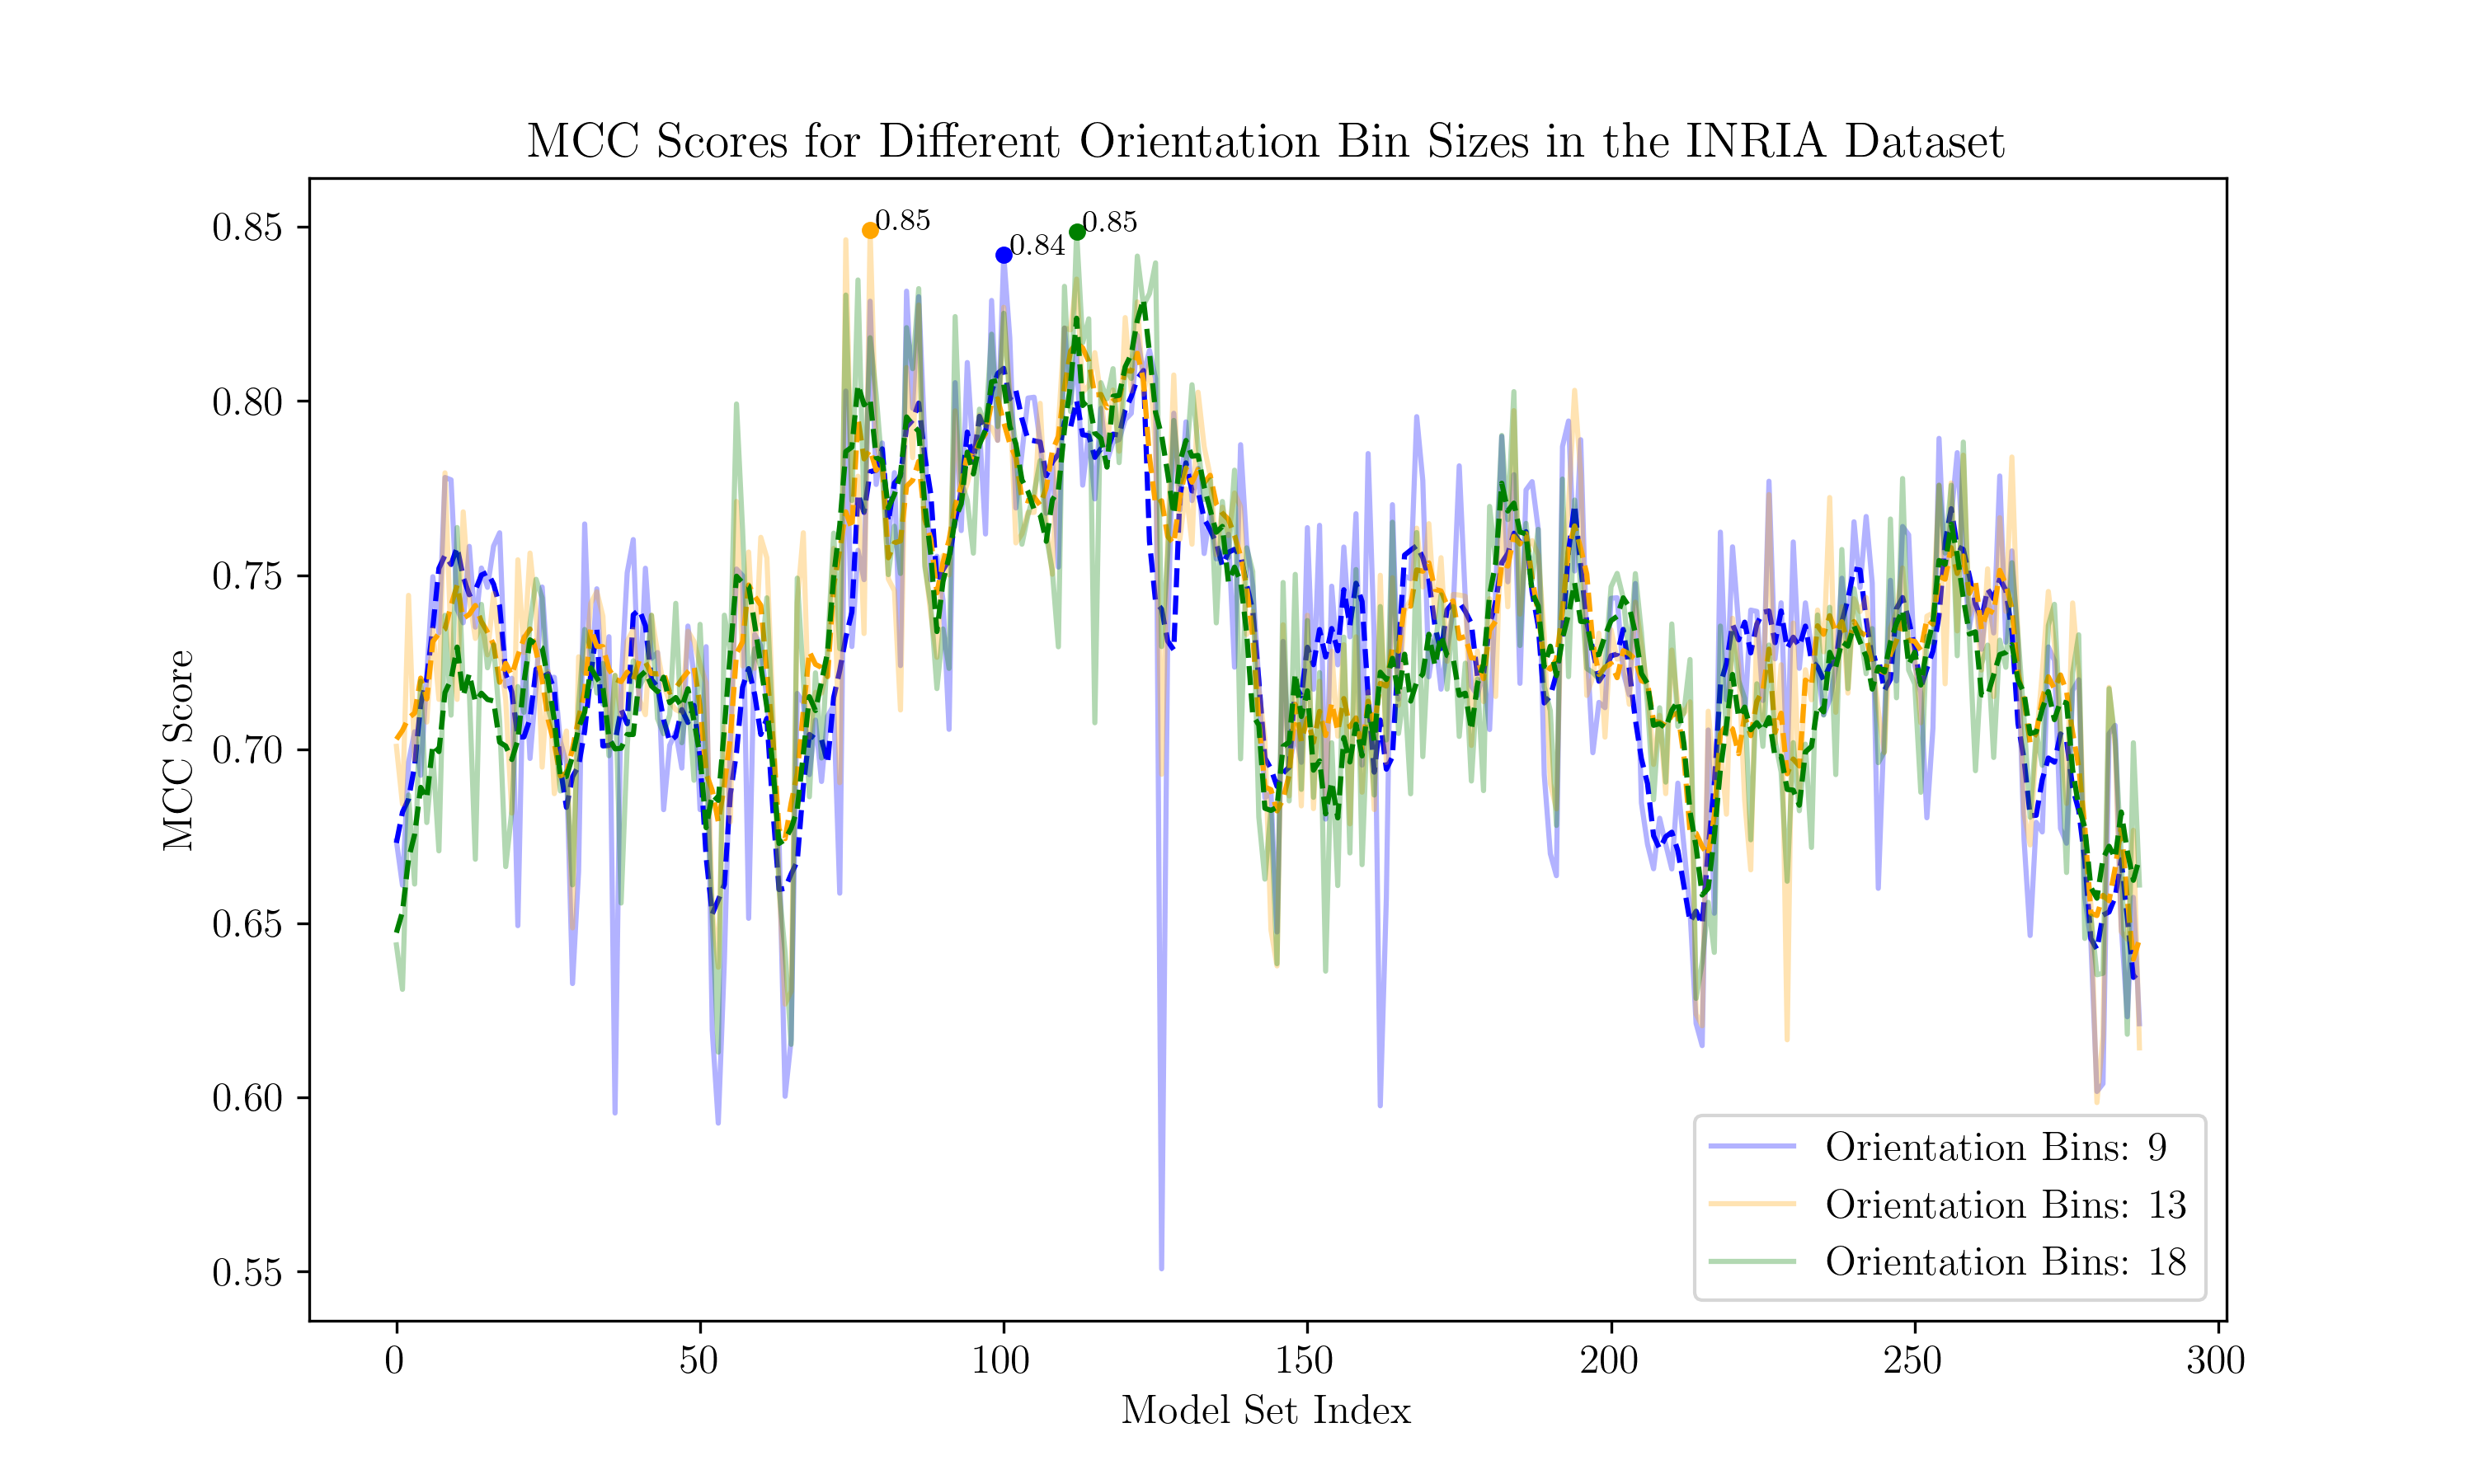
\includegraphics[width=0.9\linewidth]{mcc_bins_INRIA.png}
    \caption{
        MCC scores for INRIA dataset, grouped by orientation bin size.
    }
    \label{fig:orientation_bins_inria}
\end{figure}

\begin{figure}
    \centering
    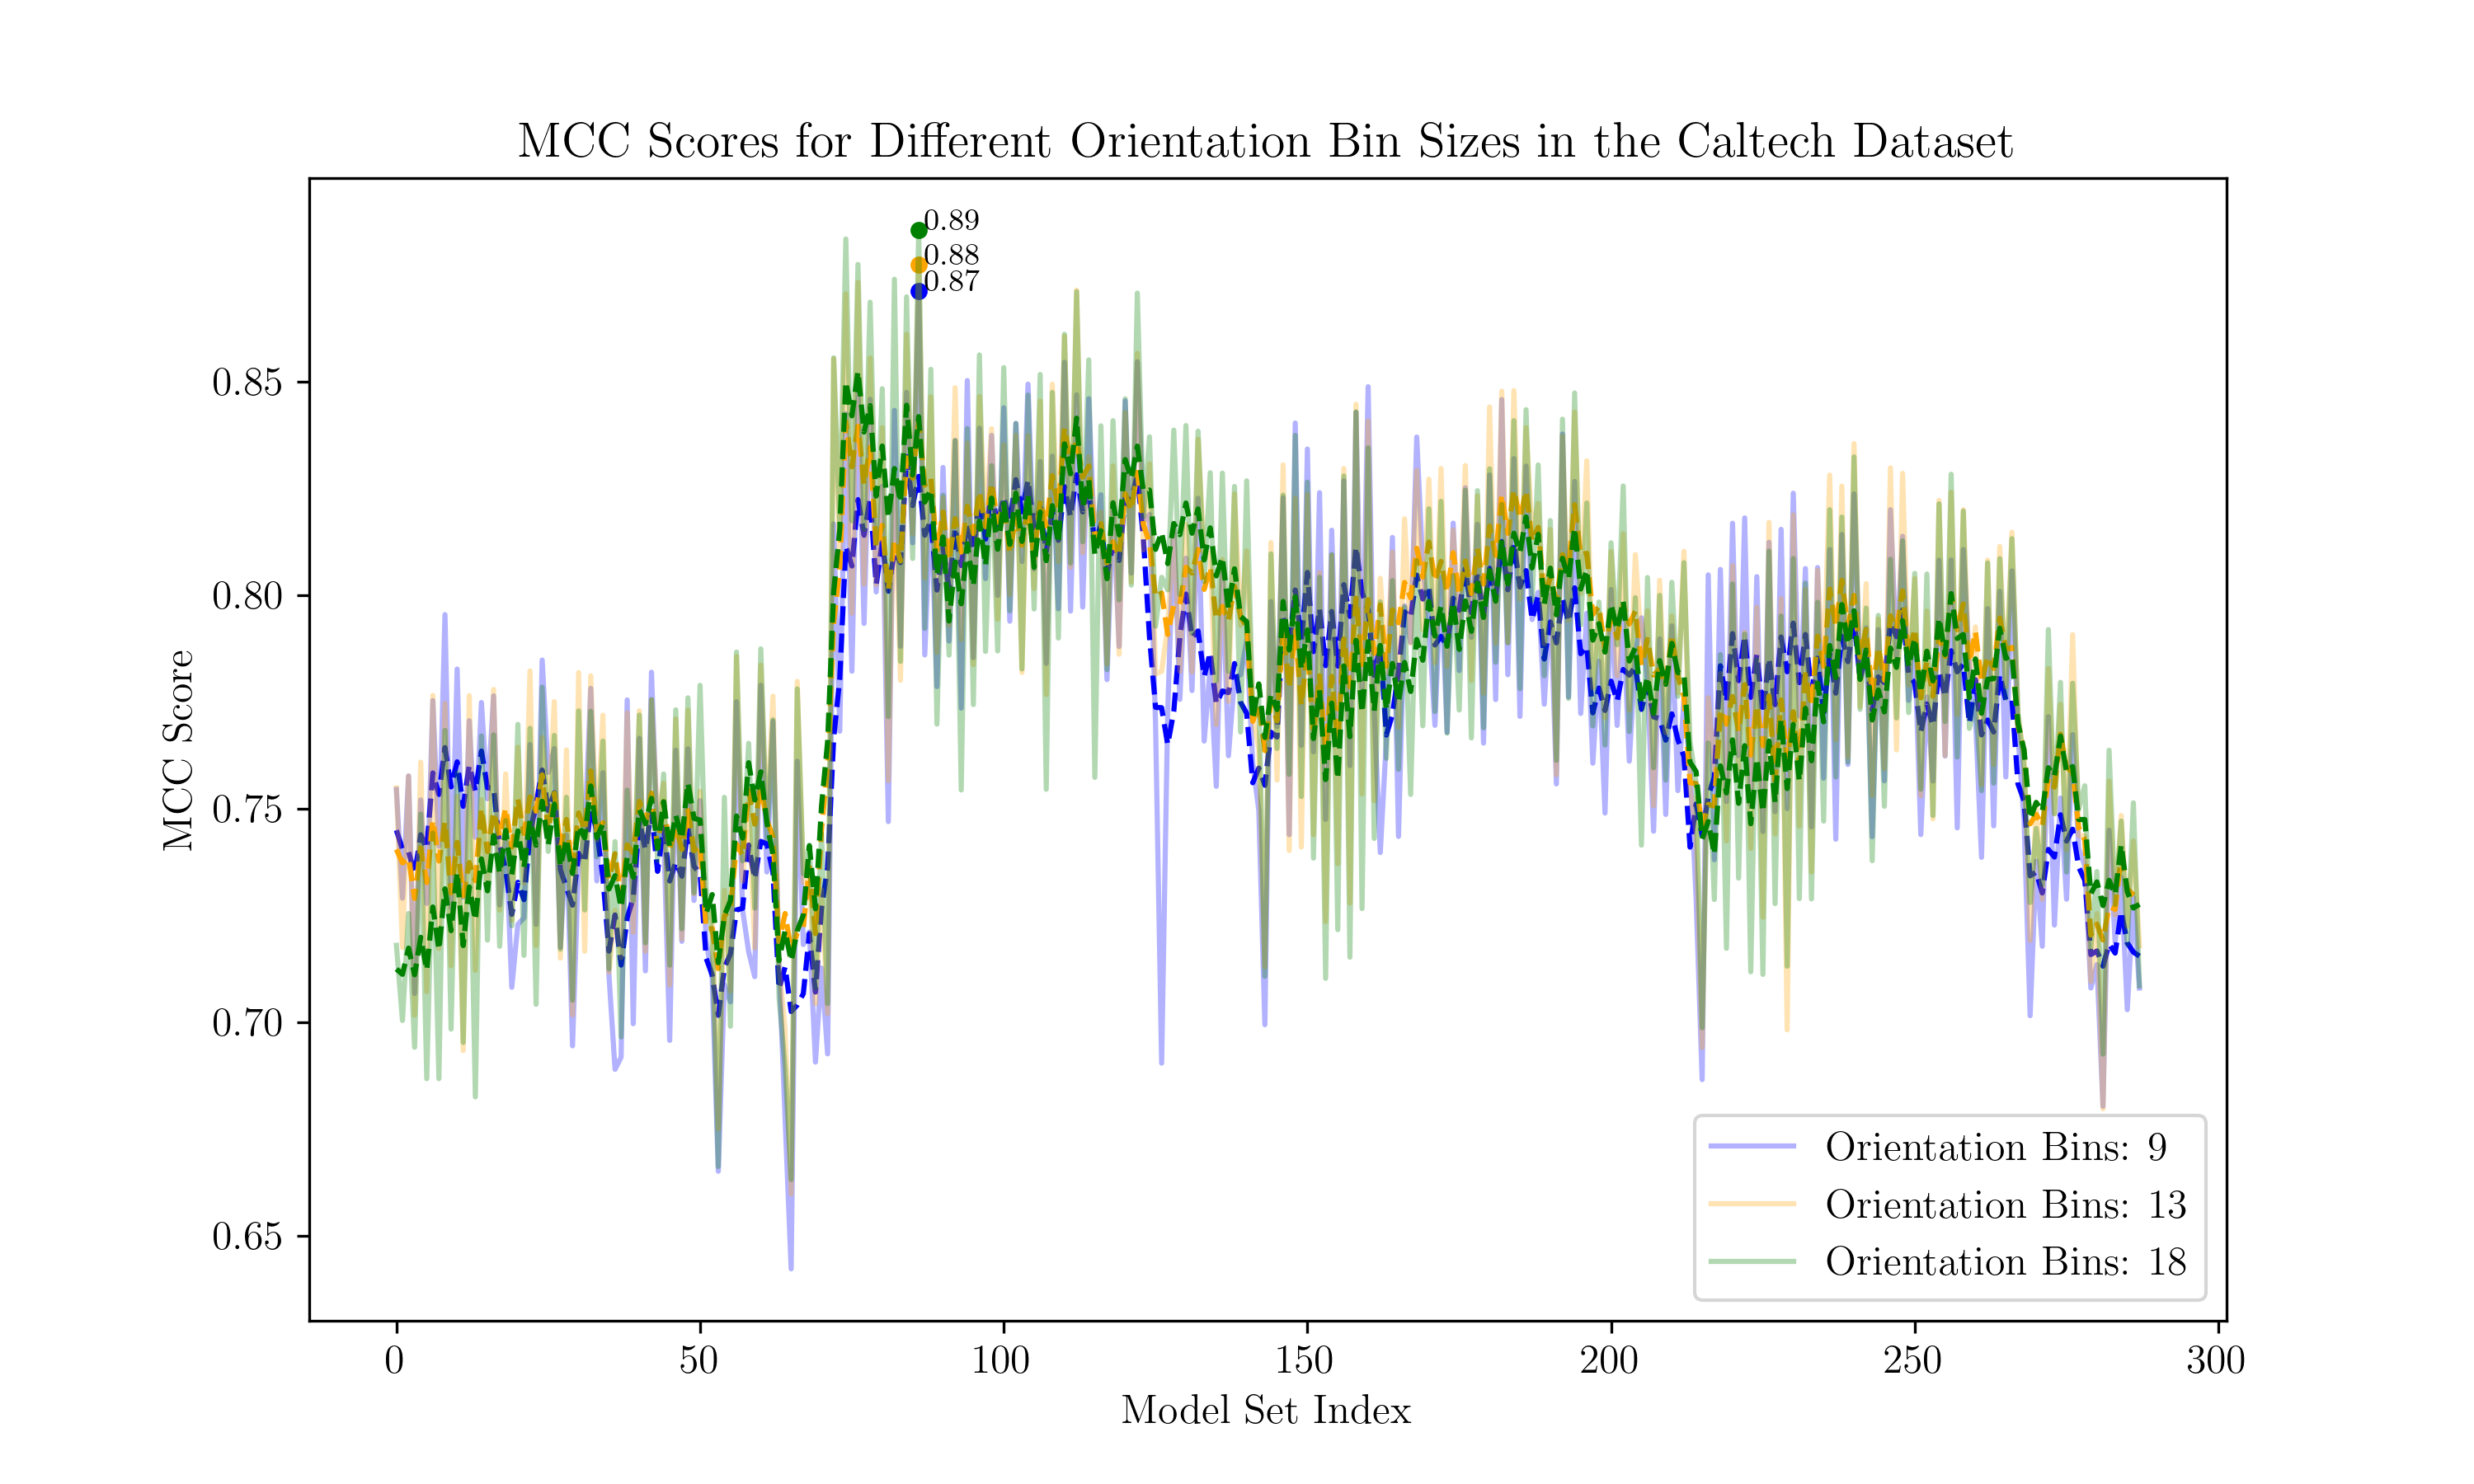
\includegraphics[width=0.9\linewidth]{mcc_bins_caltech_30.png}
    \caption{
        MCC scores for Caltech dataset, grouped by orientation bin size.
    }
\end{figure}

\begin{figure}
    \centering
    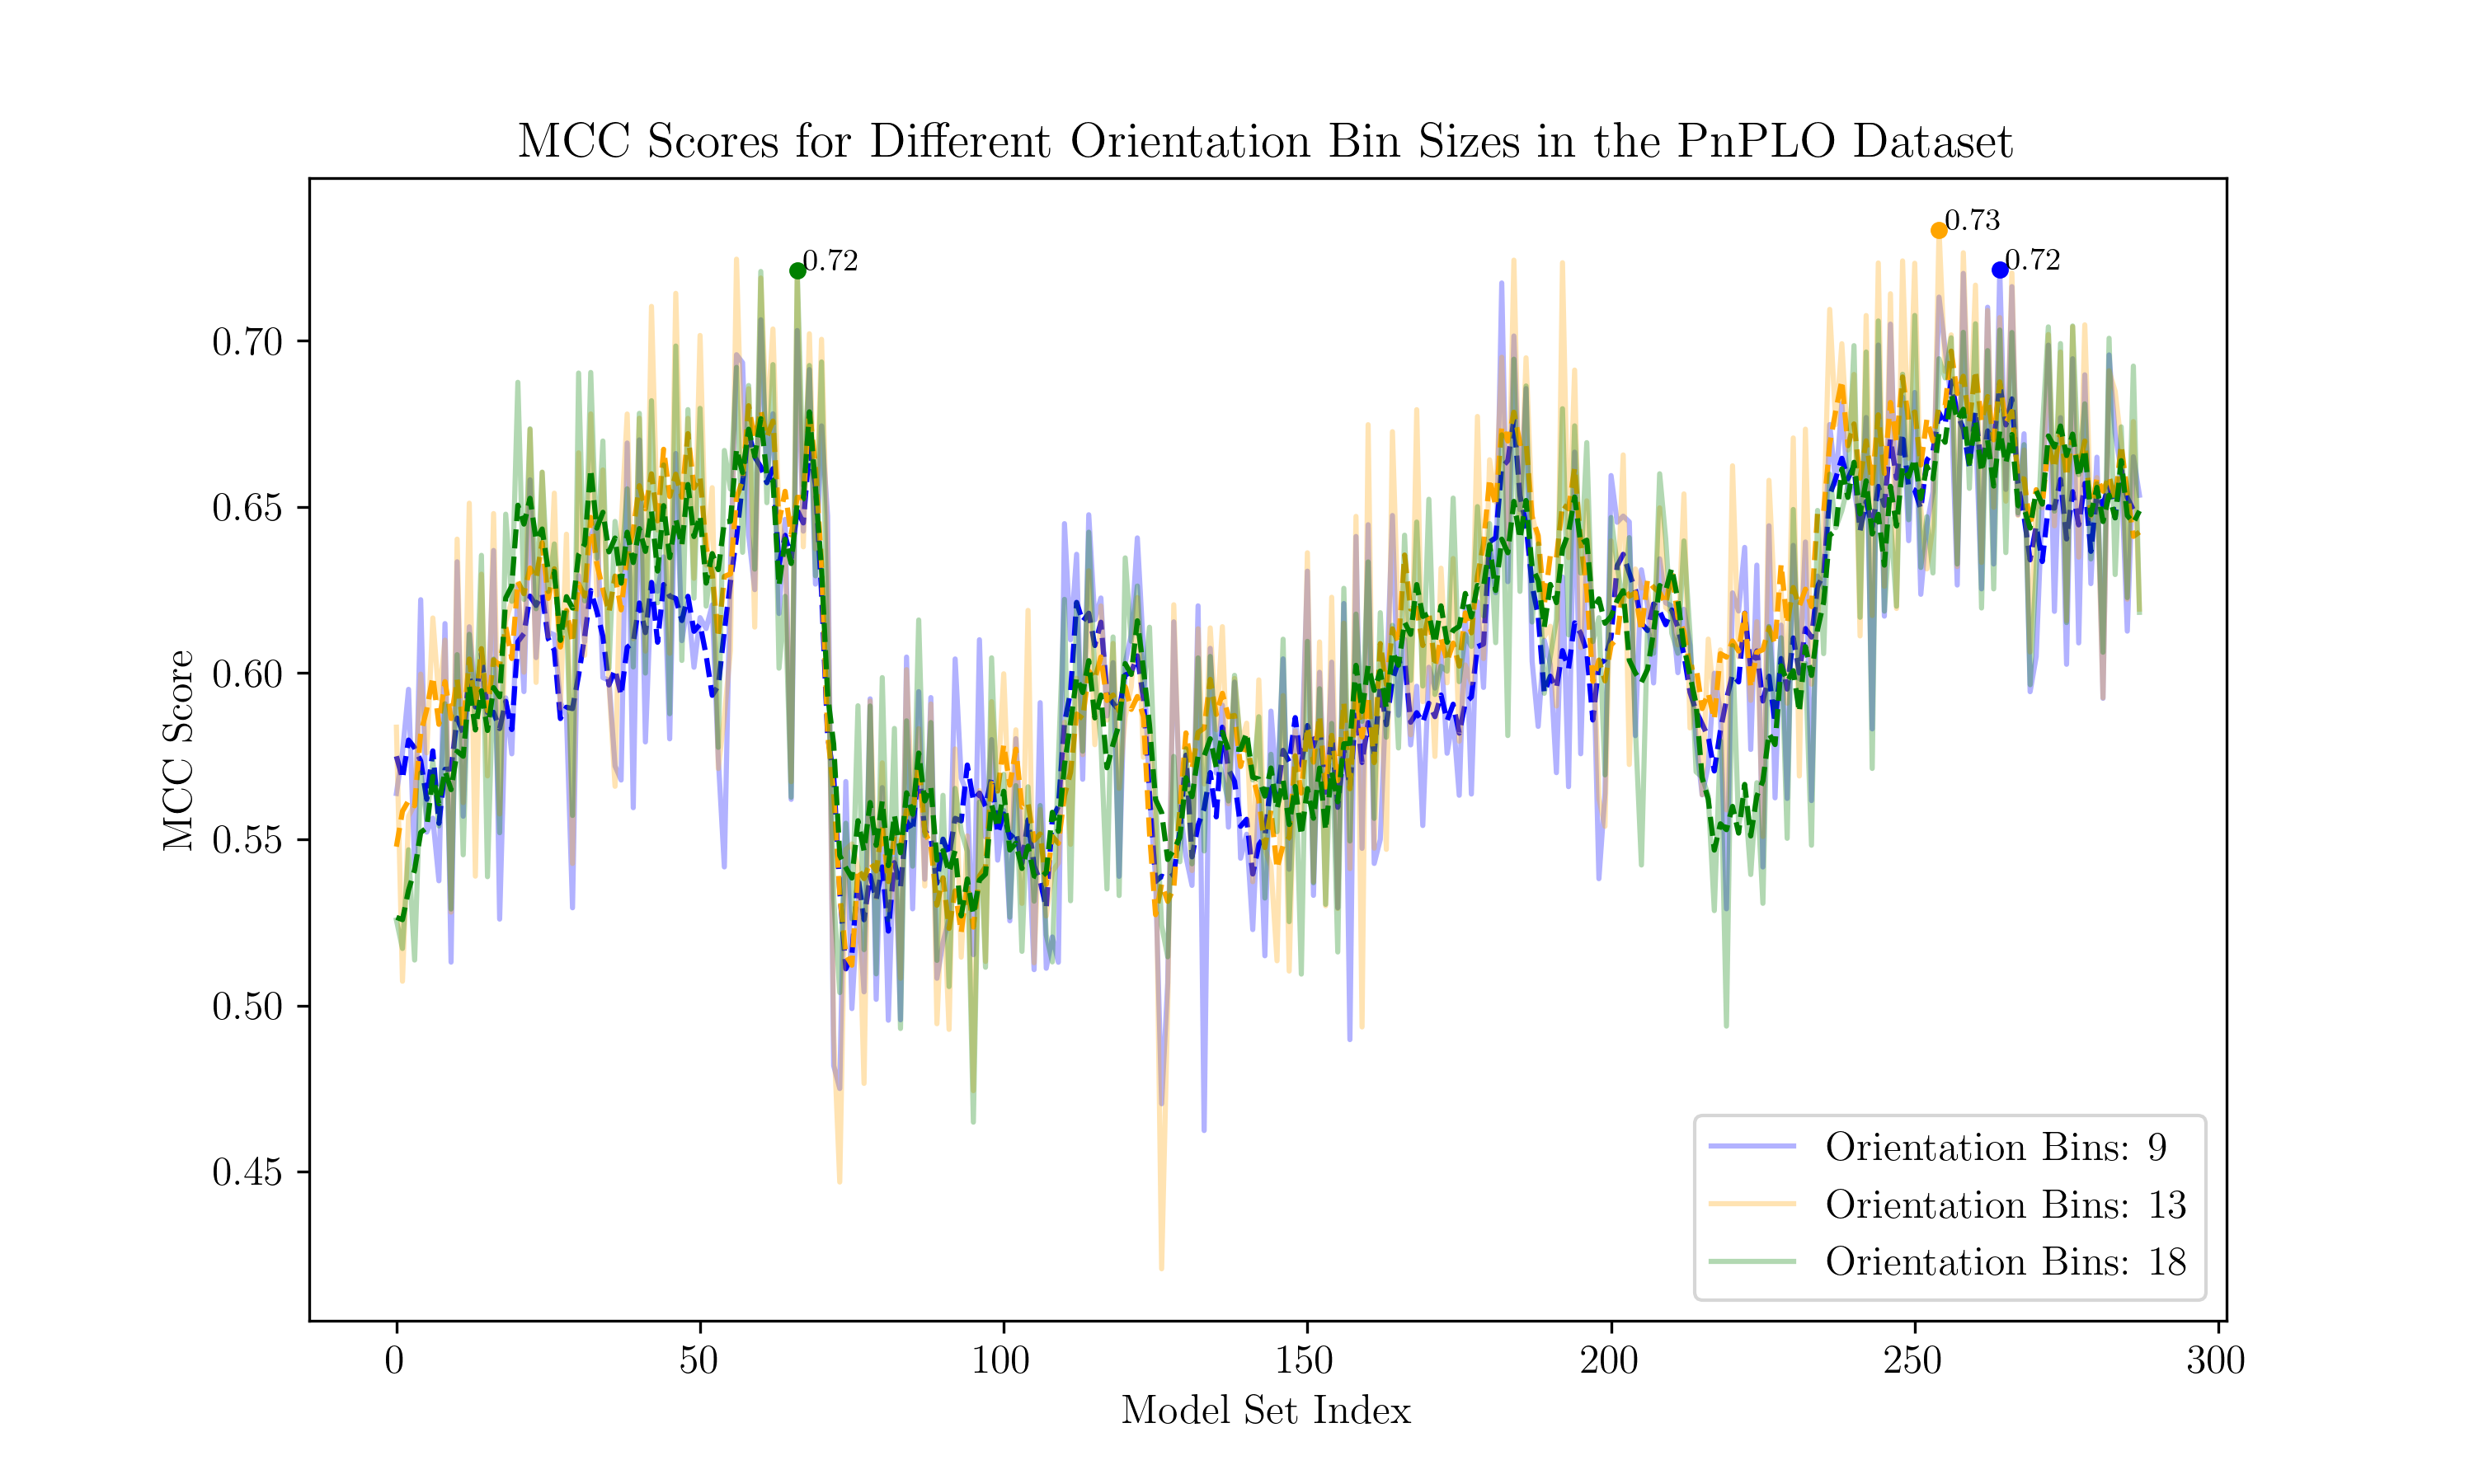
\includegraphics[width=0.9\linewidth]{mcc_bins_PnPLO.png}
    \caption{
        MCC scores for PnPLO dataset, grouped by orientation bin size.
    }
\end{figure}

\begin{figure}
    \centering
    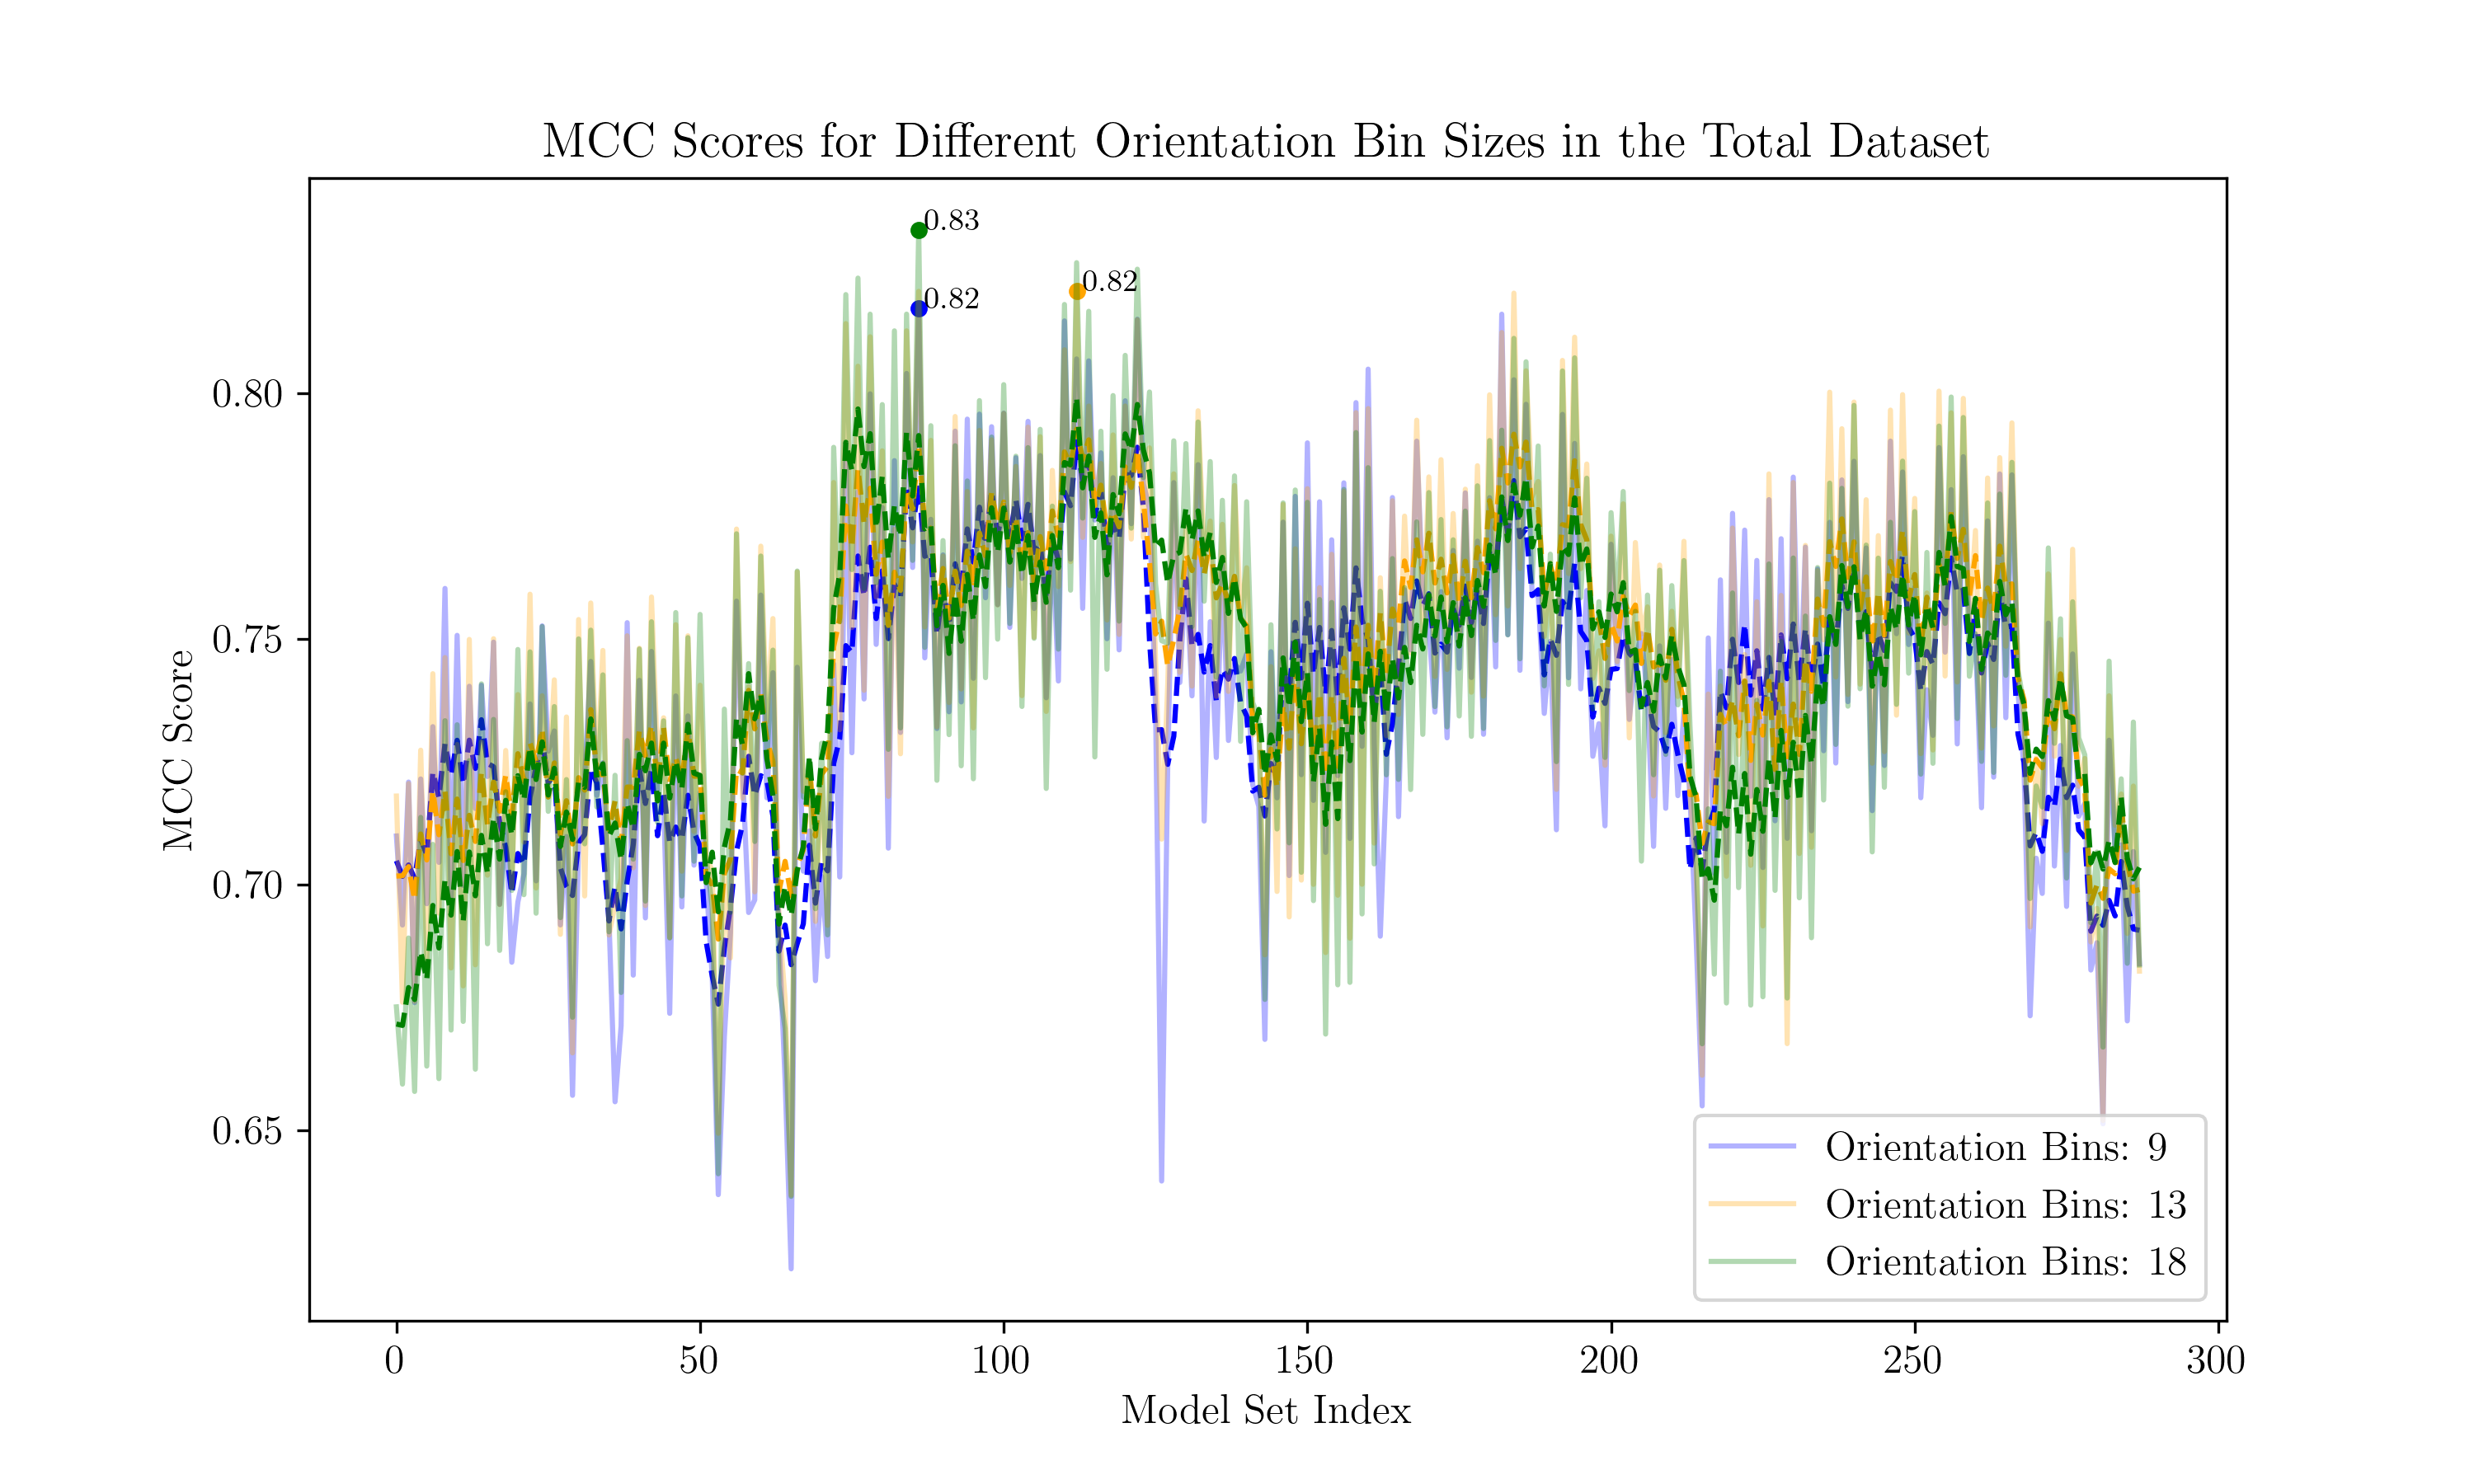
\includegraphics[width=0.9\linewidth]{mcc_bins_total.png}
    \caption{
        MCC scores for the aggregate test dataset, grouped by orientation bin size.
    }
    \label{fig:orientation_bins_total}
\end{figure}


\subsubsection{Graphs for Different Cell Sizes}

\begin{figure}
    \centering
    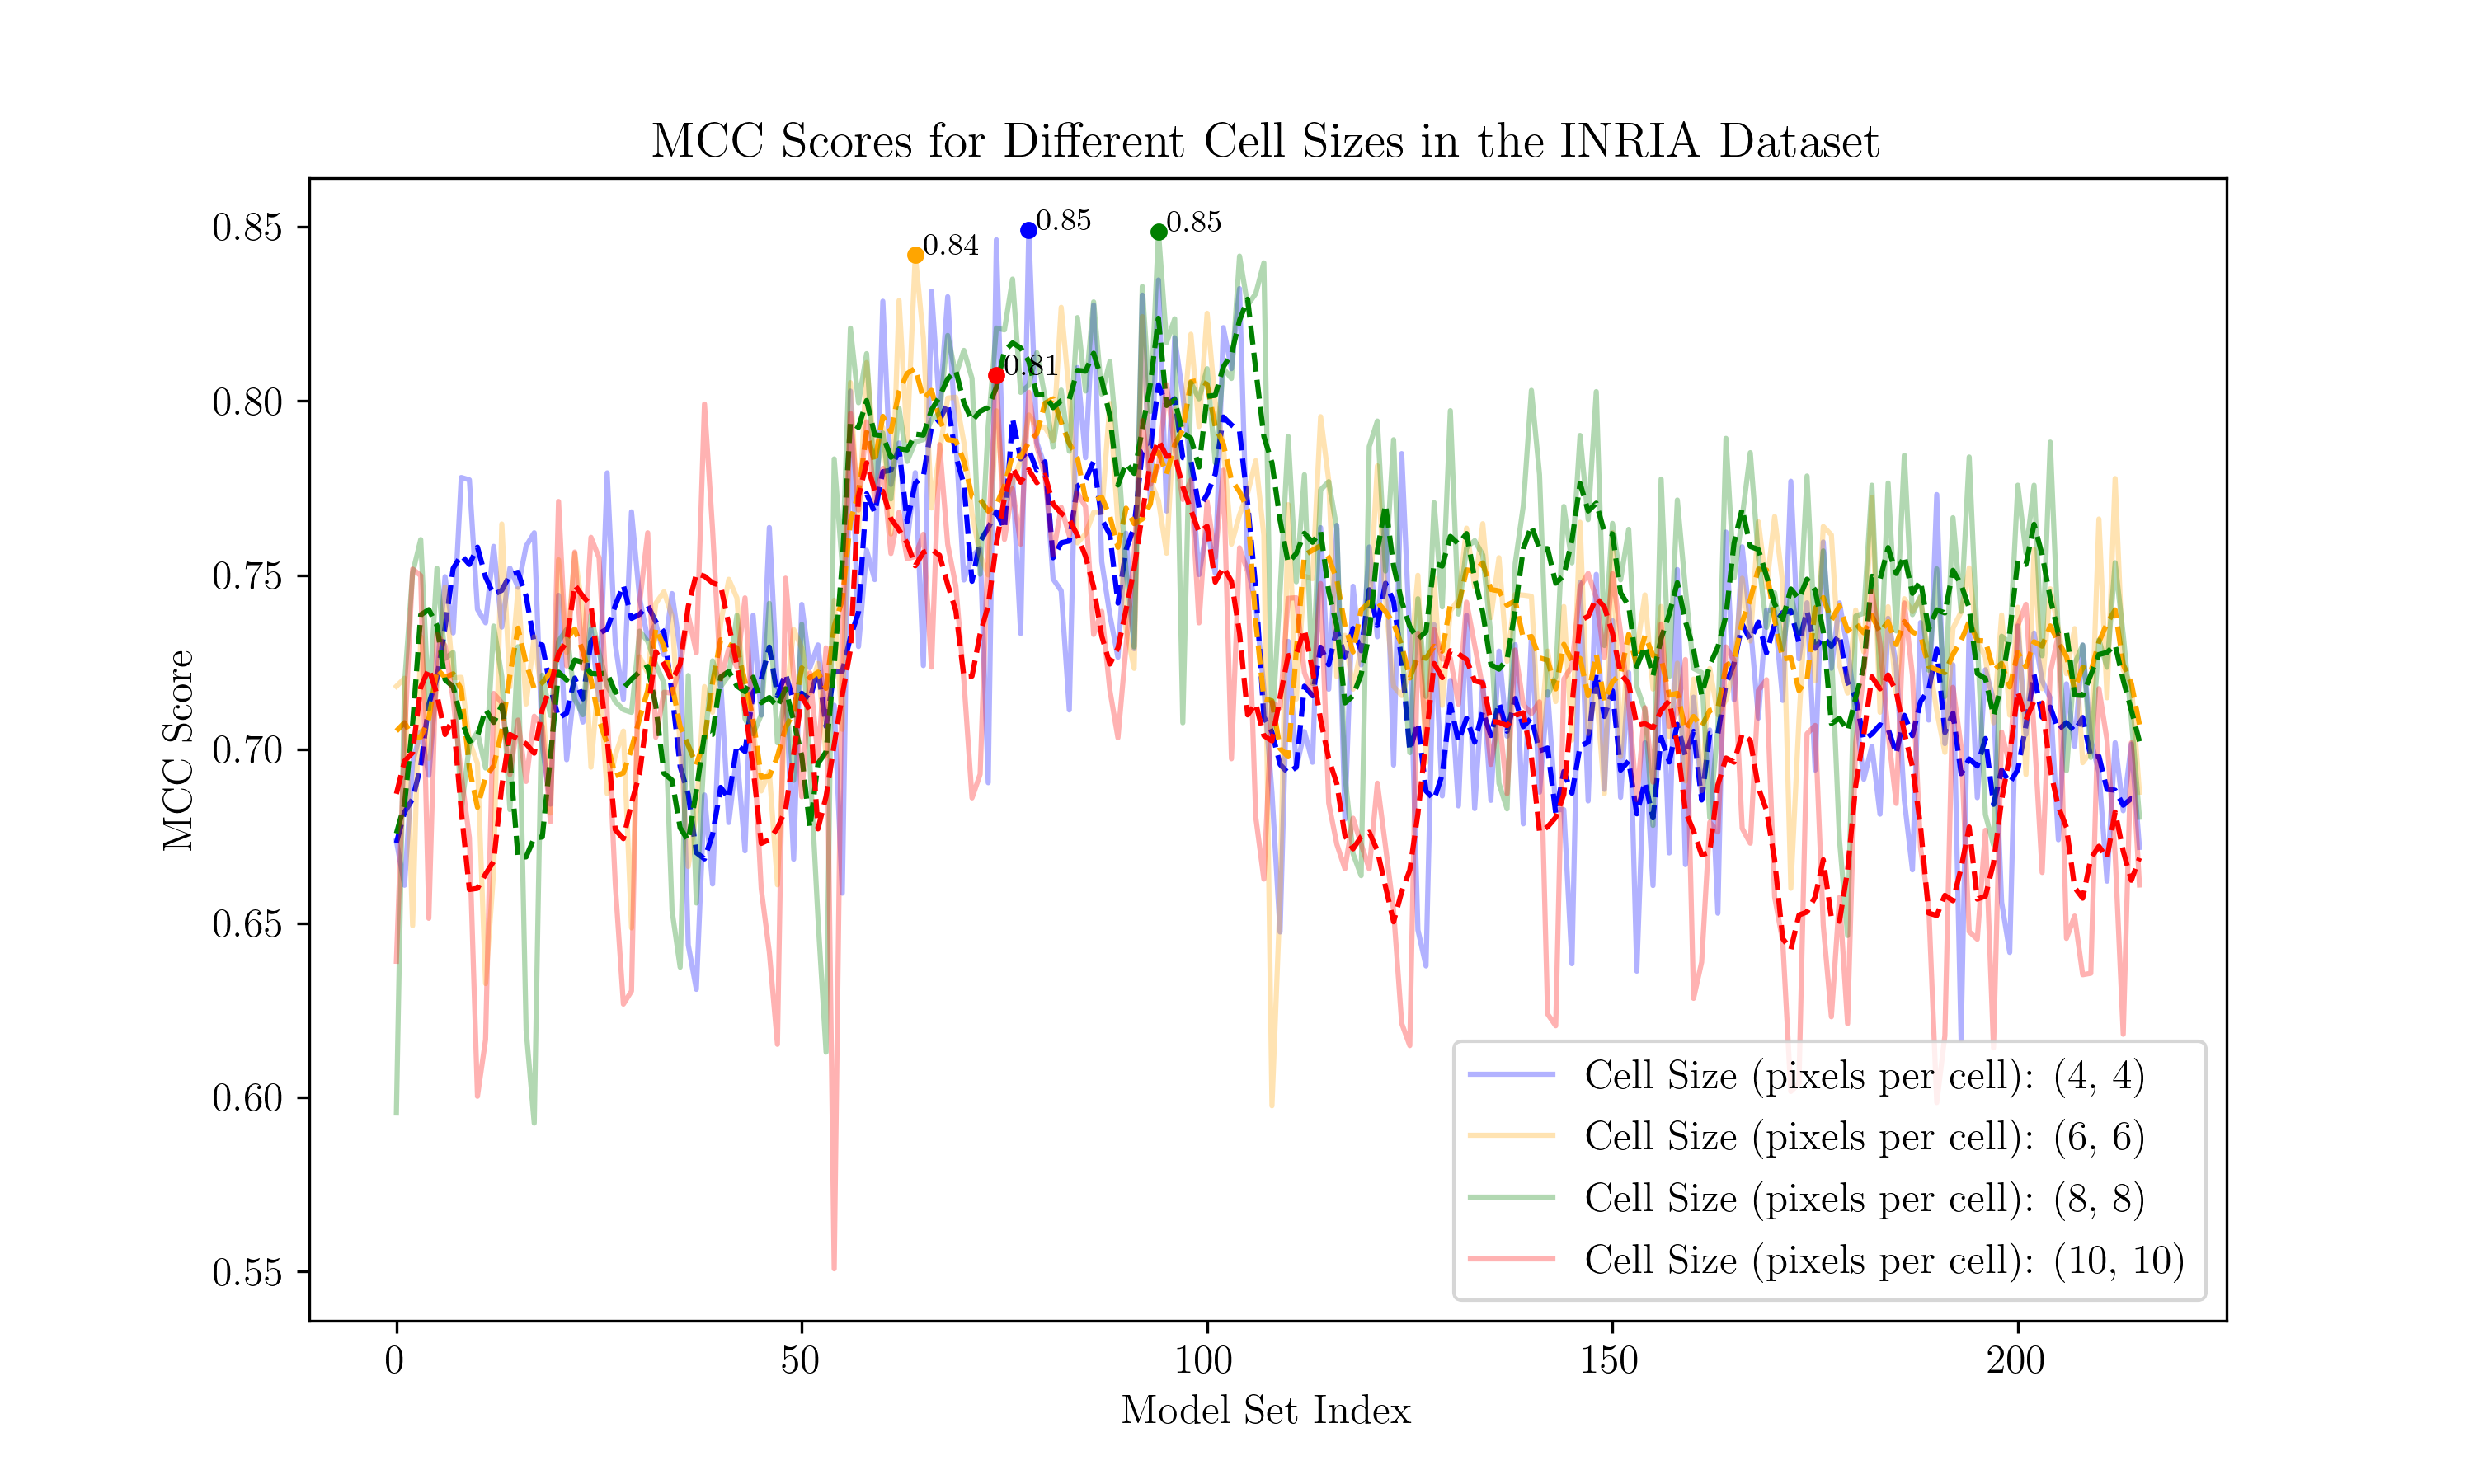
\includegraphics[width=0.9\linewidth]{mcc_cell_size_INRIA.png}
    \caption{
        MCC scores for INRIA dataset, grouped by cell size.
    }
\end{figure}

\begin{figure}
    \centering
    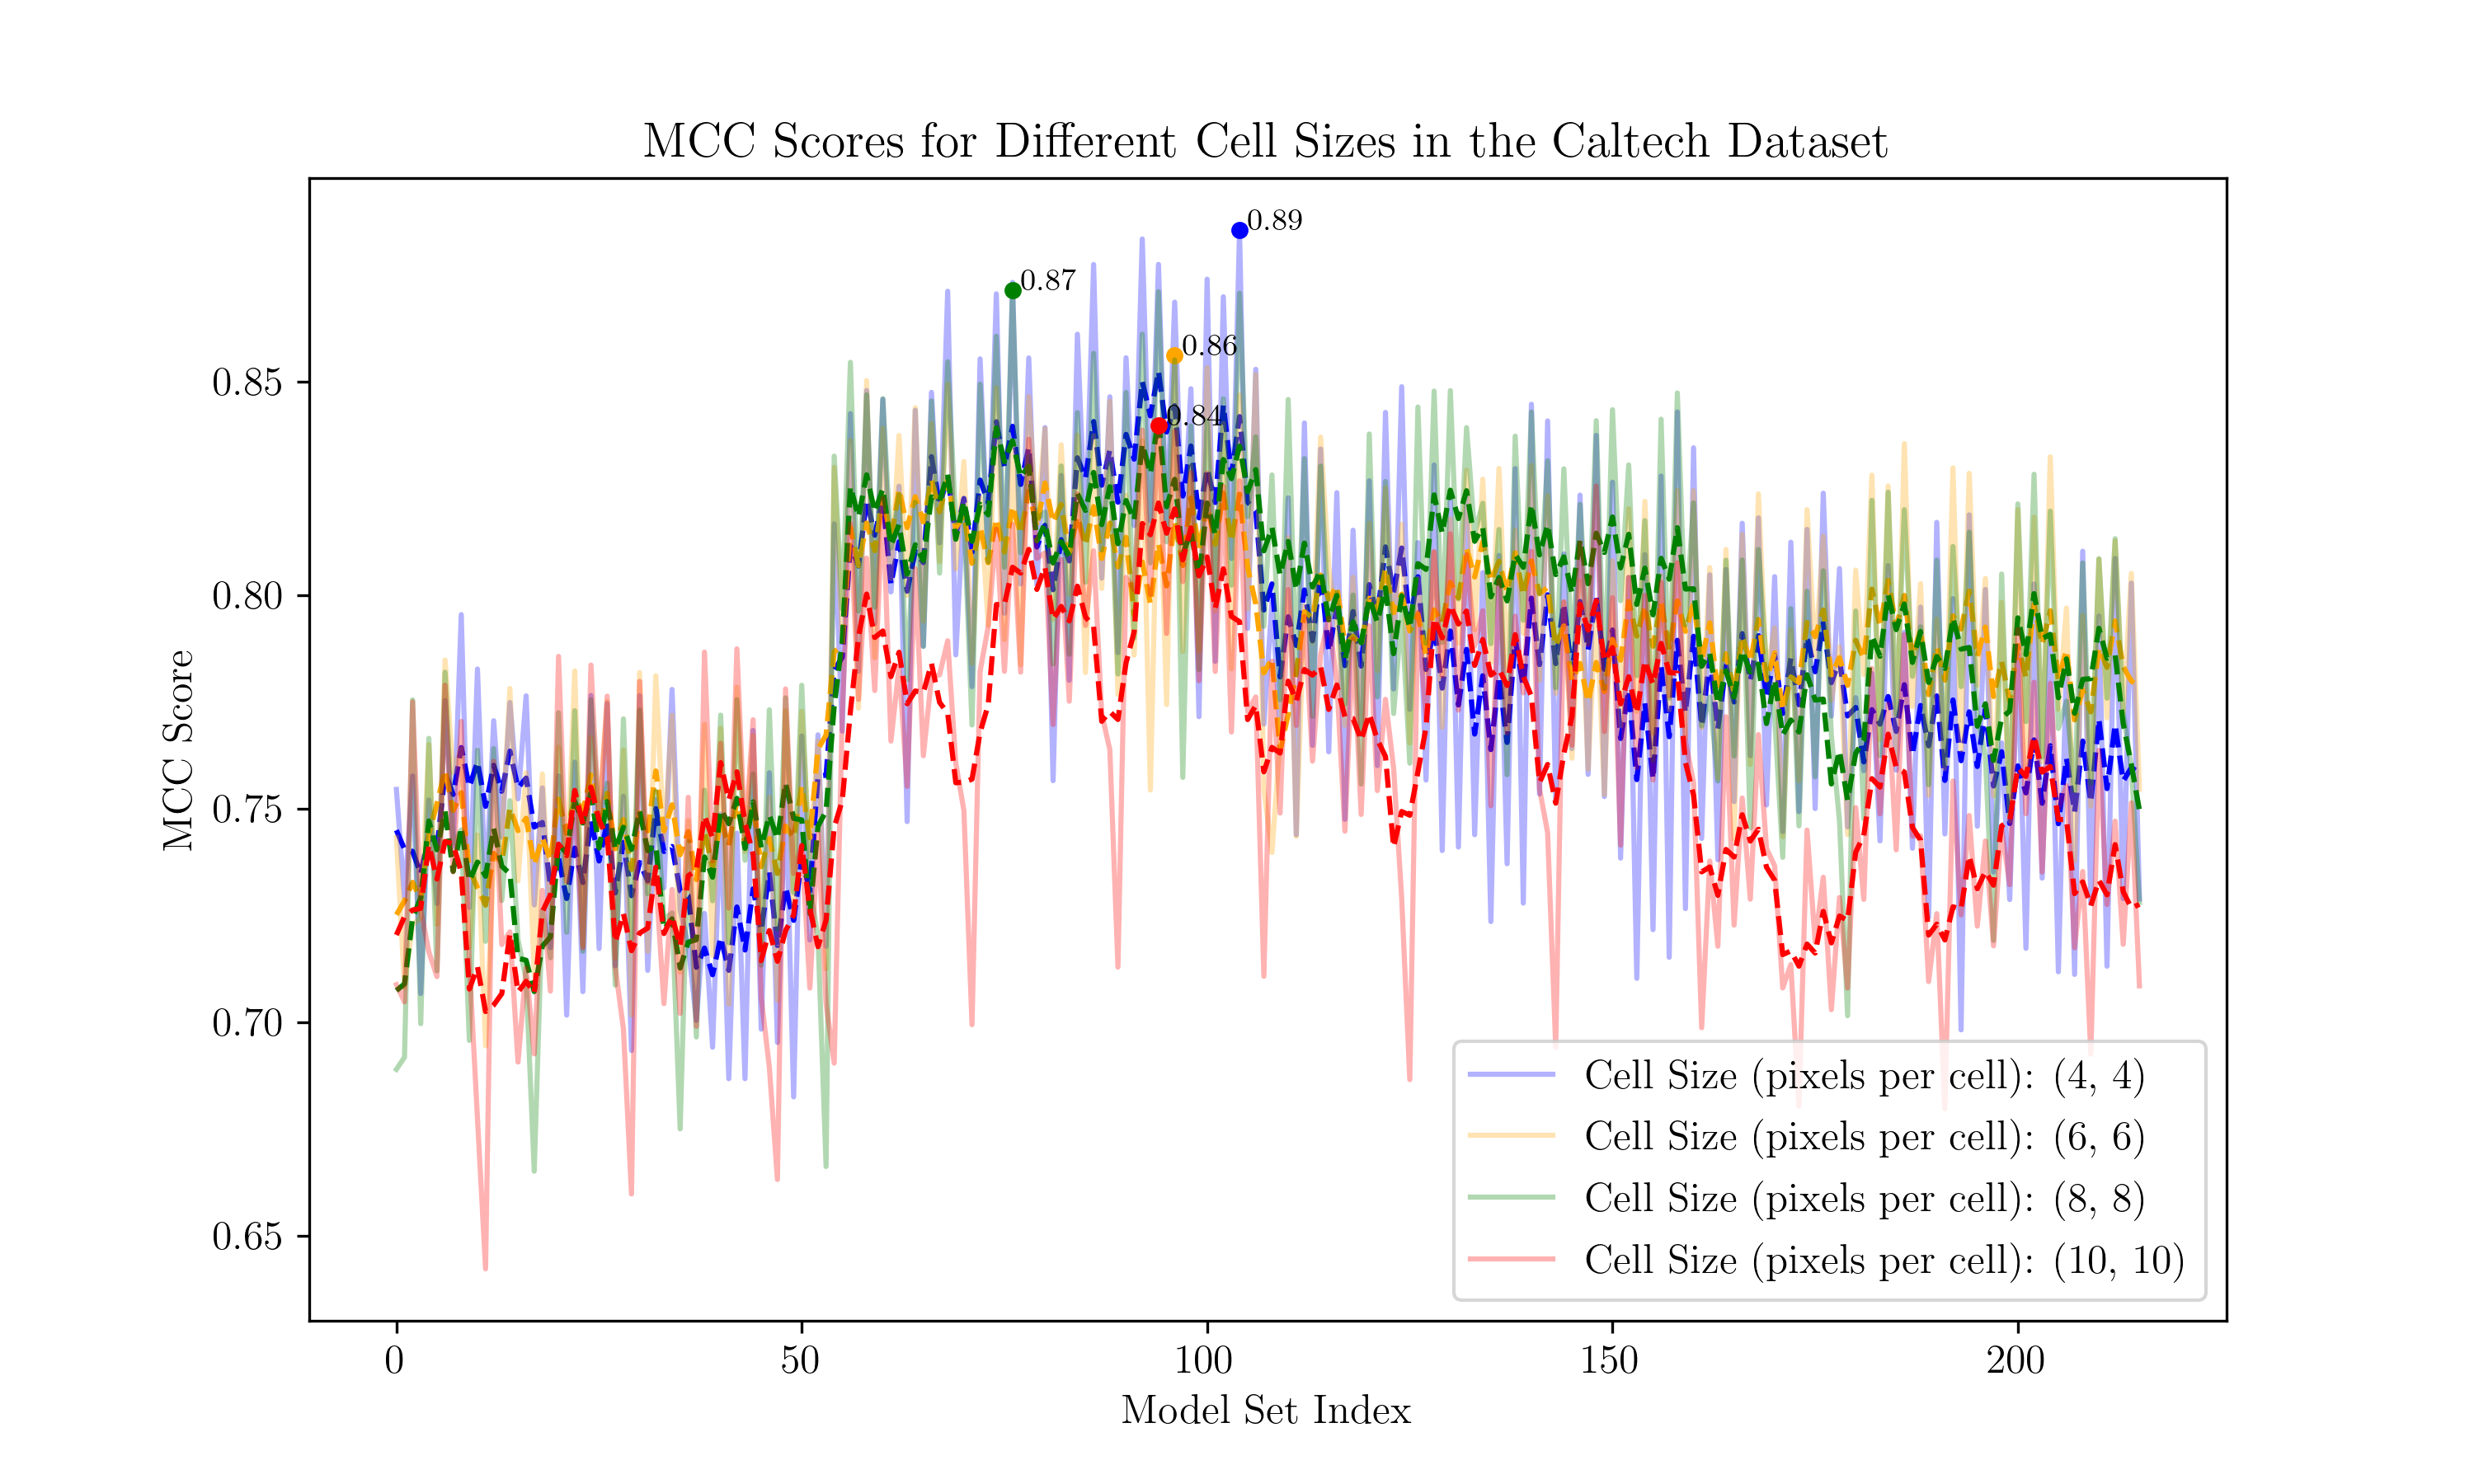
\includegraphics[width=0.9\linewidth]{mcc_cell_size_caltech_30.png}
    \caption{
        MCC scores for Caltech dataset, grouped by cell size.
    }
\end{figure}

\begin{figure}
    \centering
    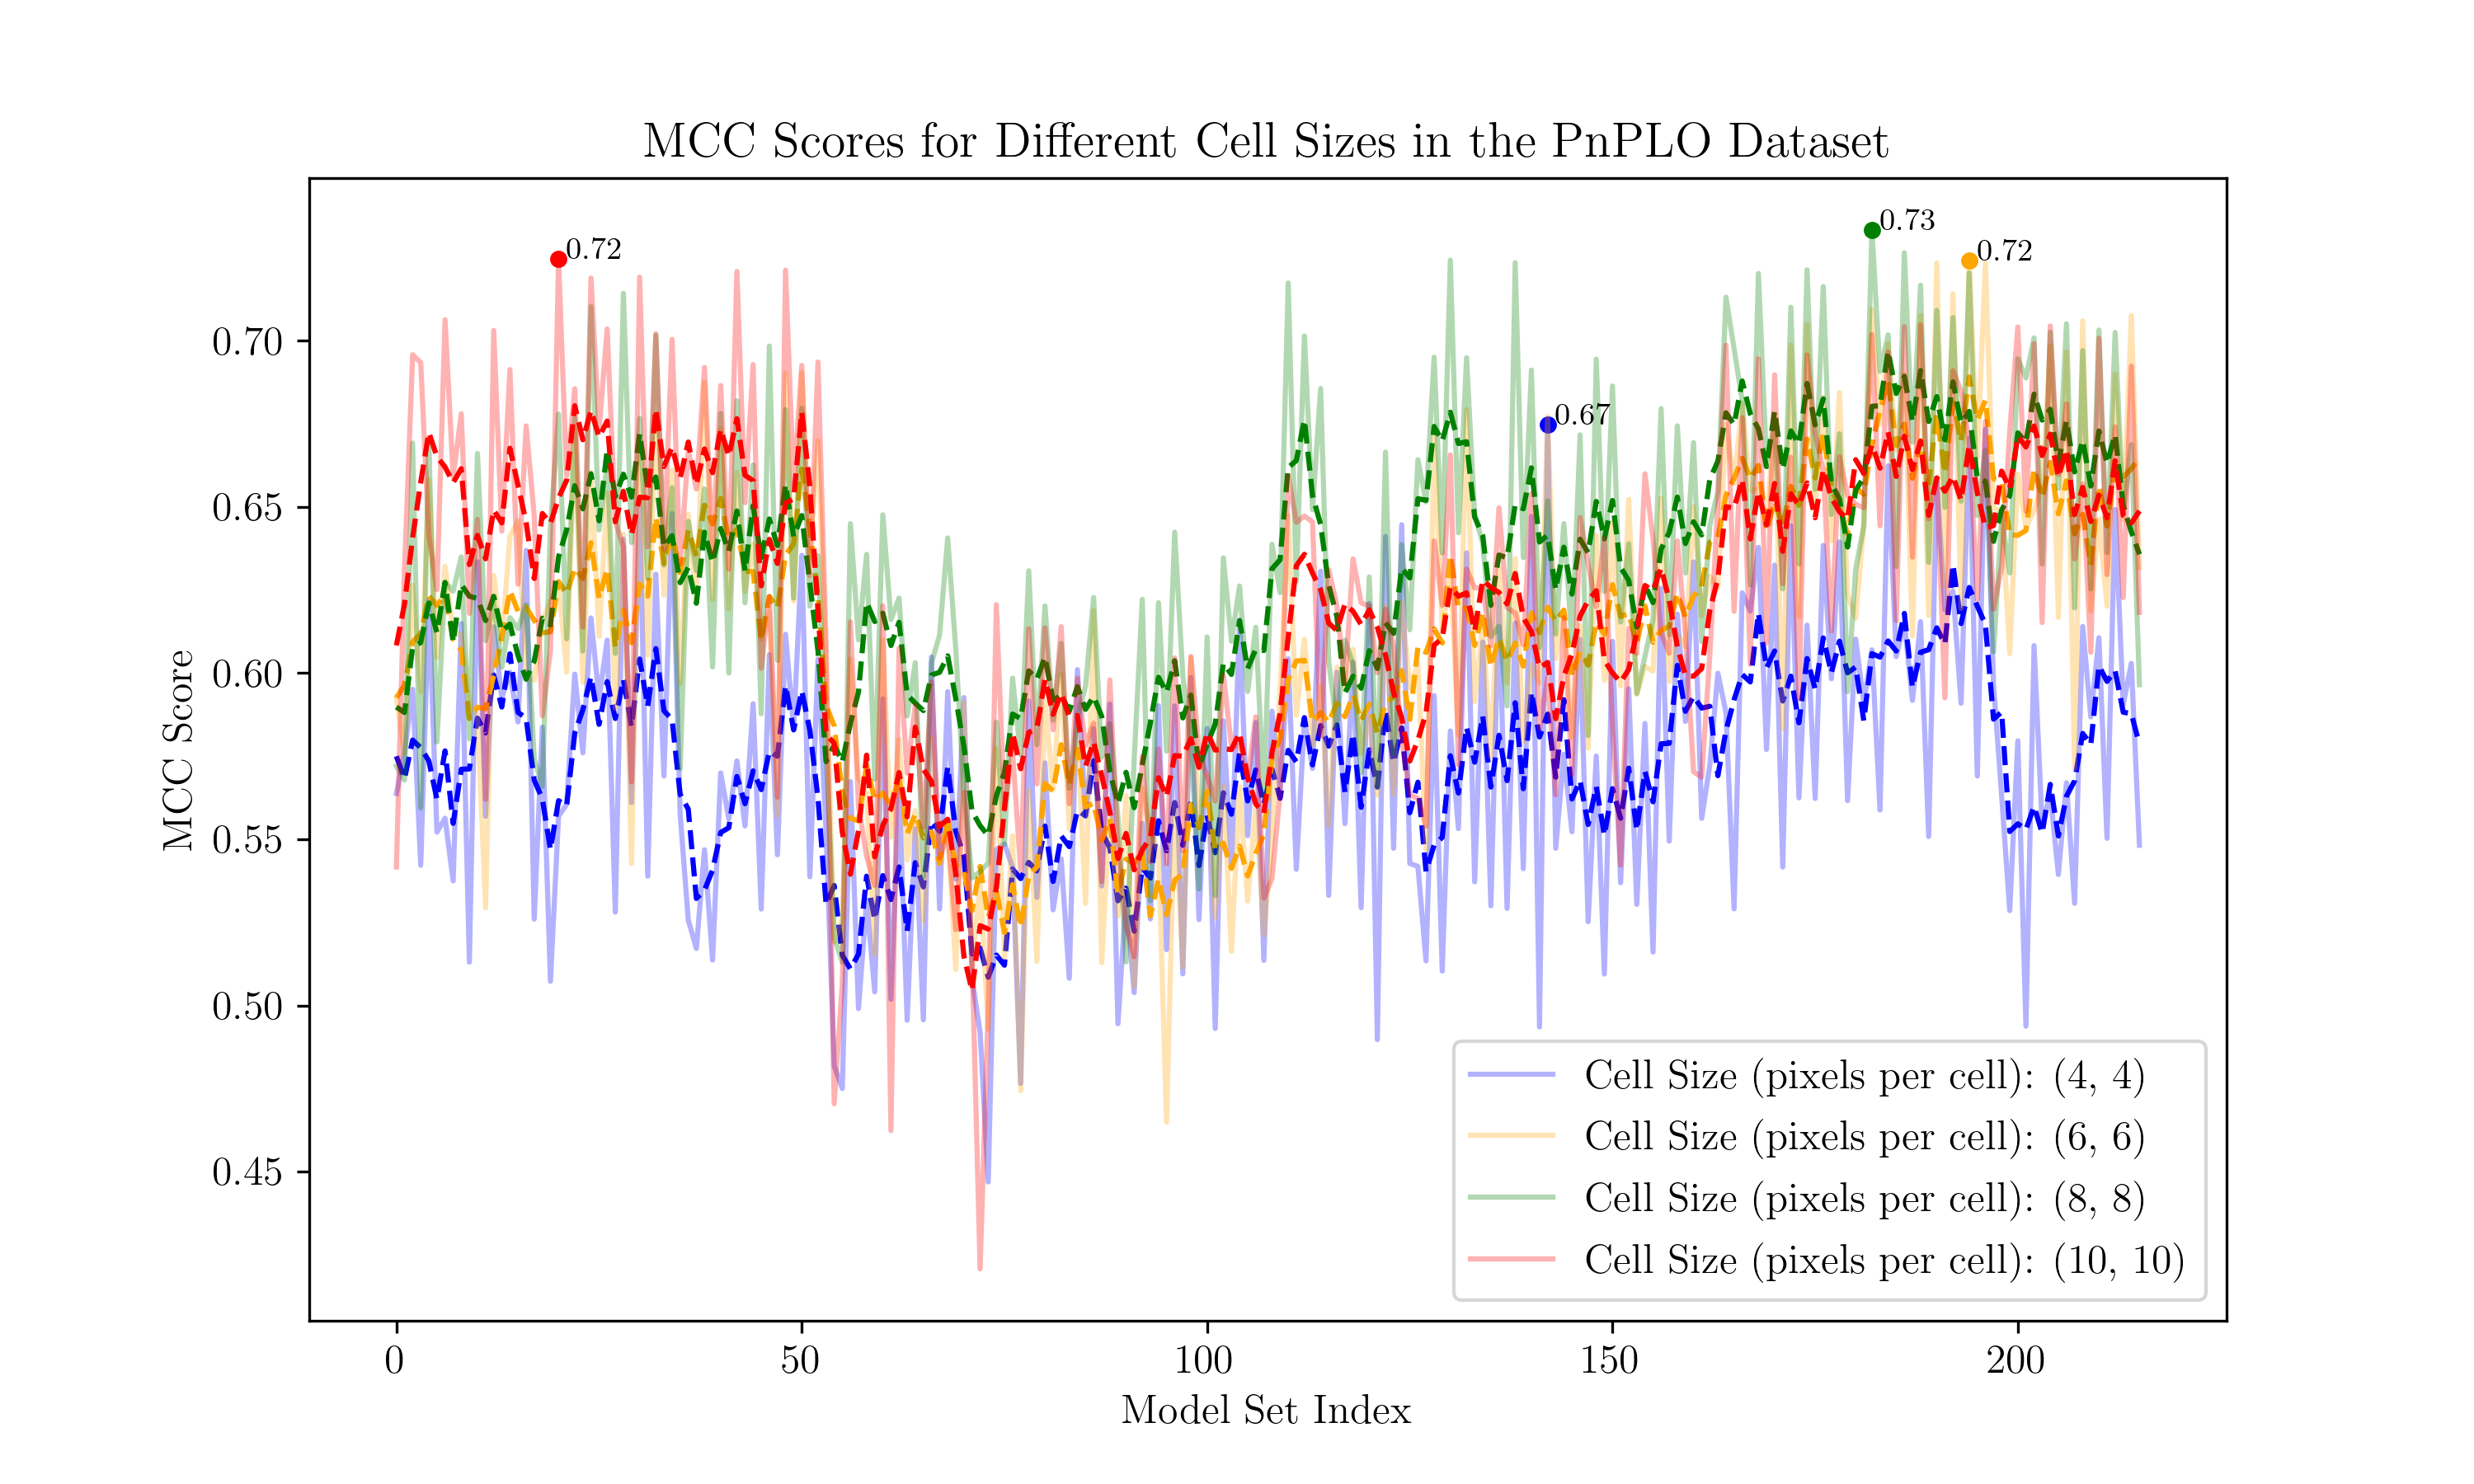
\includegraphics[width=0.9\linewidth]{mcc_cell_size_PnPLO.png}
    \caption{
        MCC scores for PnPLO dataset, grouped by cell size.
    }
\end{figure}

\begin{figure}
    \centering
    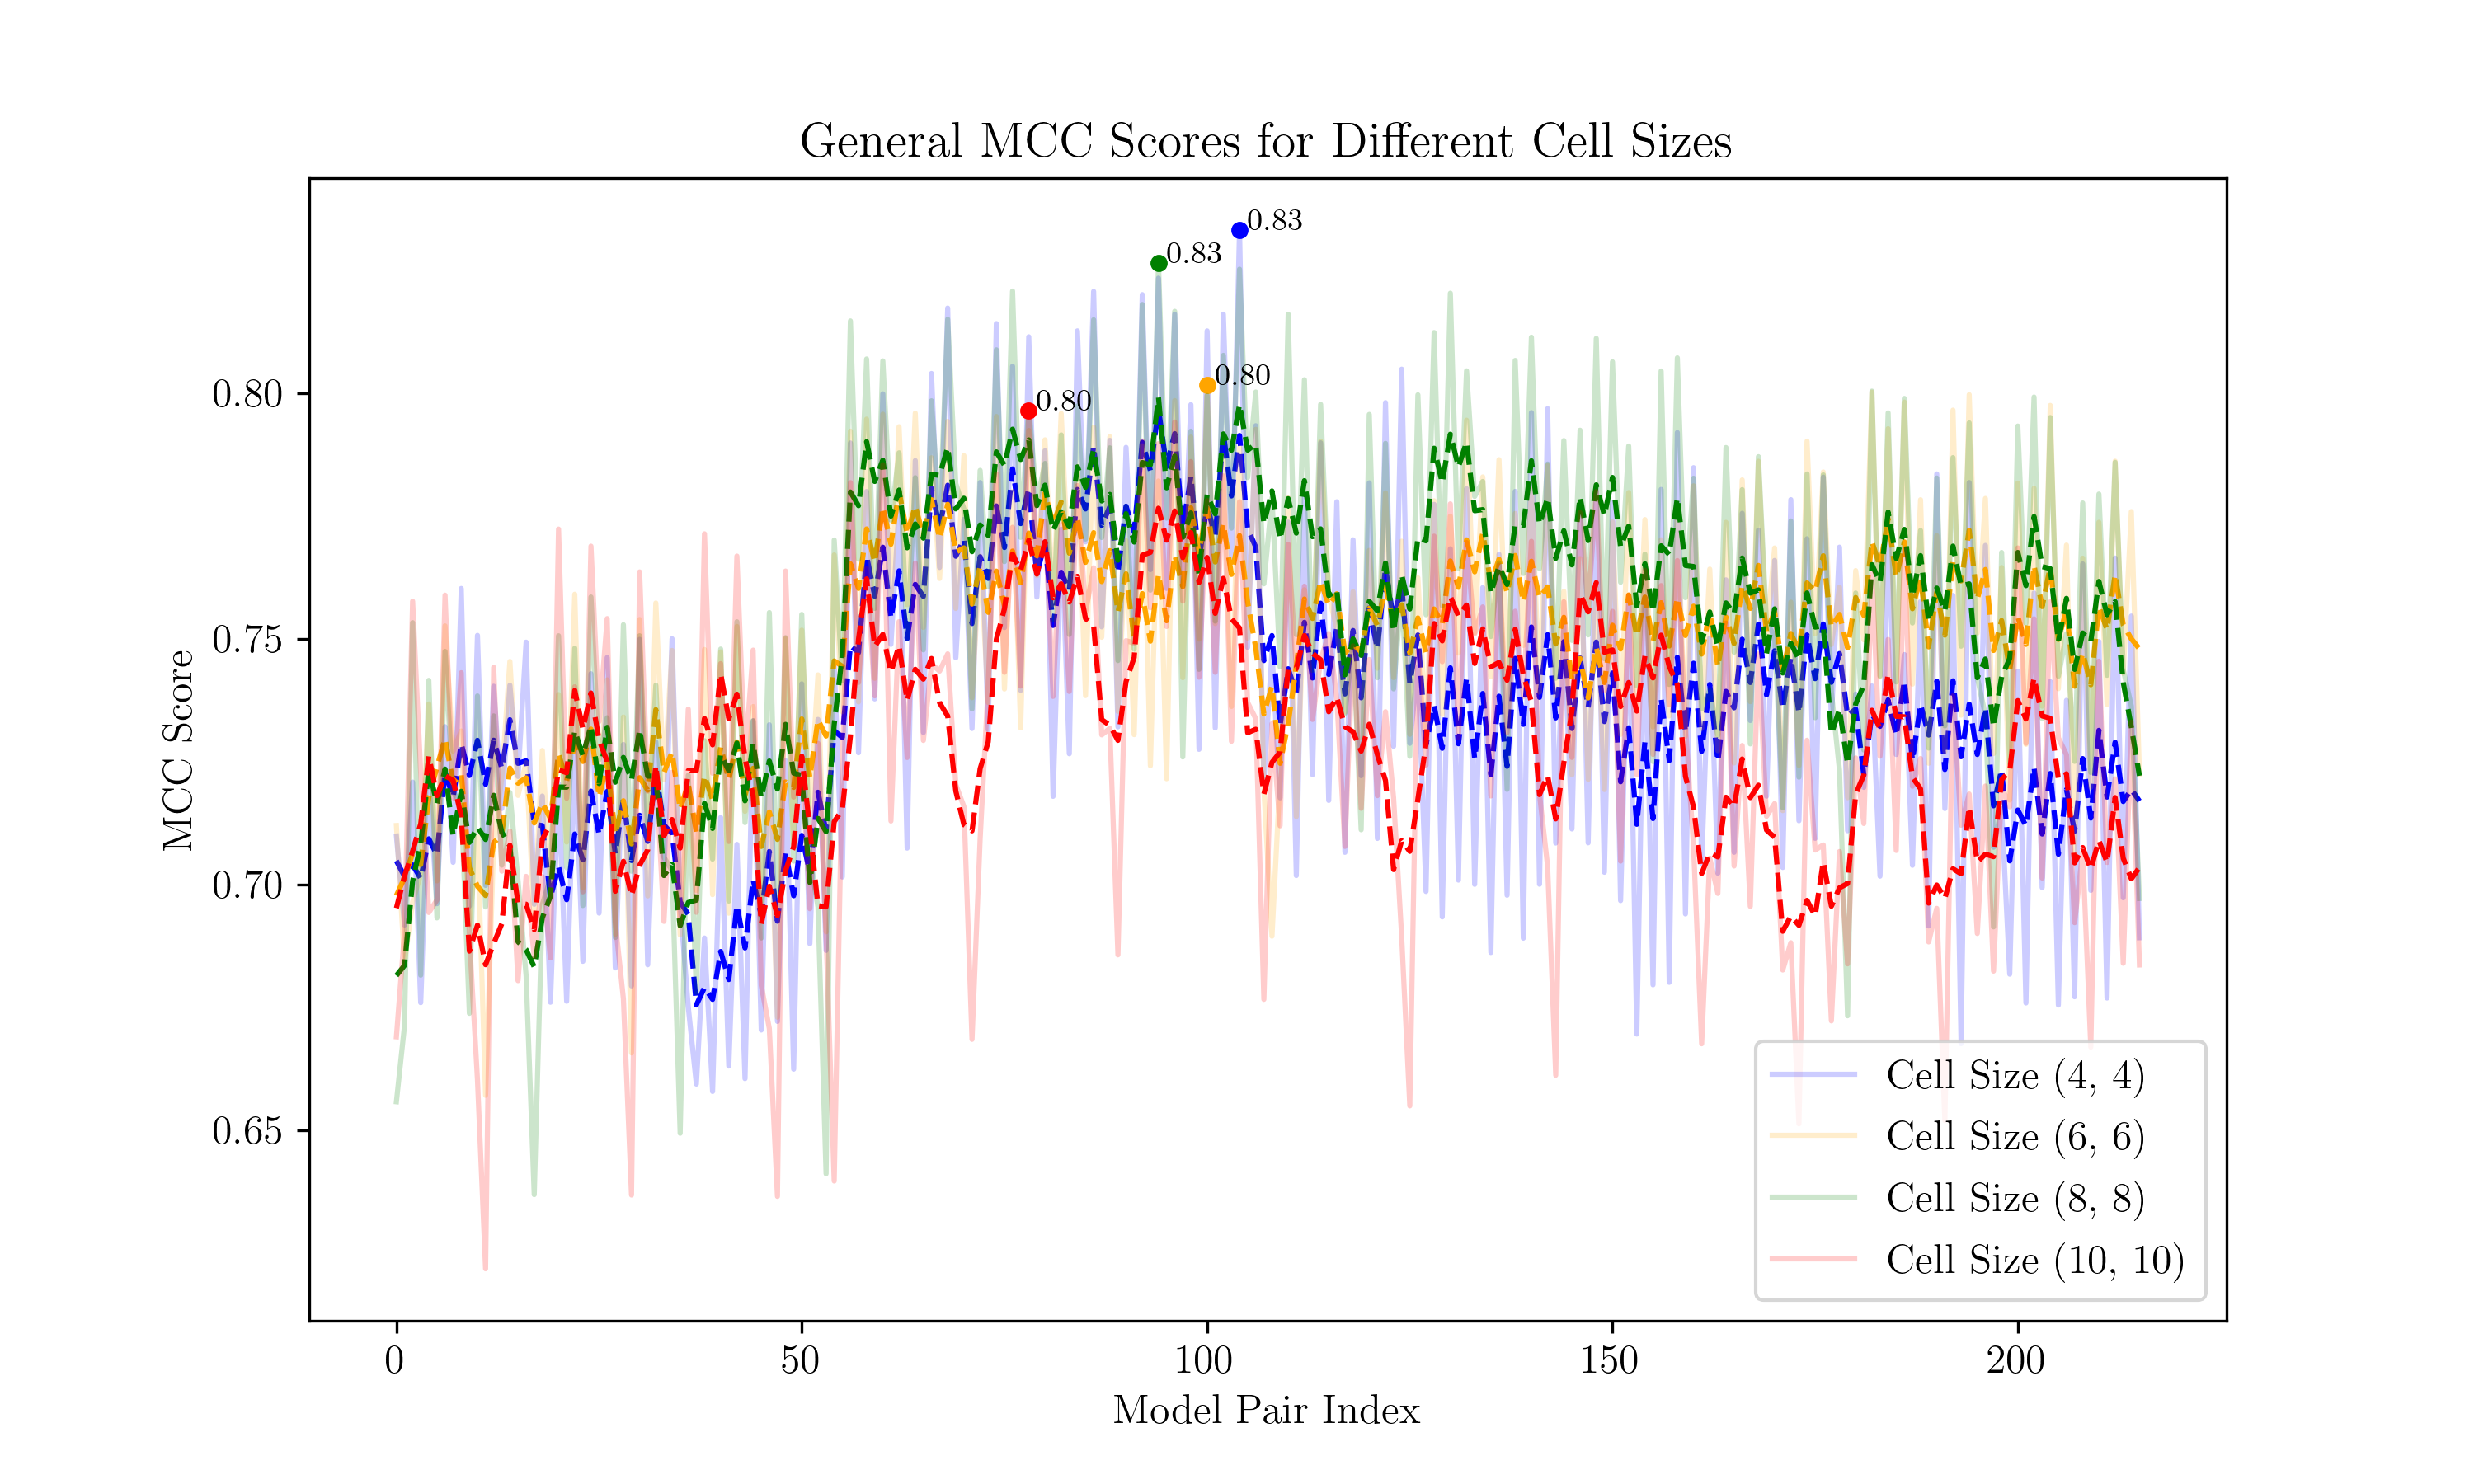
\includegraphics[width=0.9\linewidth]{mcc_cell_size_total.png}
    \caption{
        MCC scores for the aggregate test dataset, grouped by cell size.
    }
\end{figure}

\subsubsection{Graphs for Different Block Sizes}

\begin{figure}
    \centering
    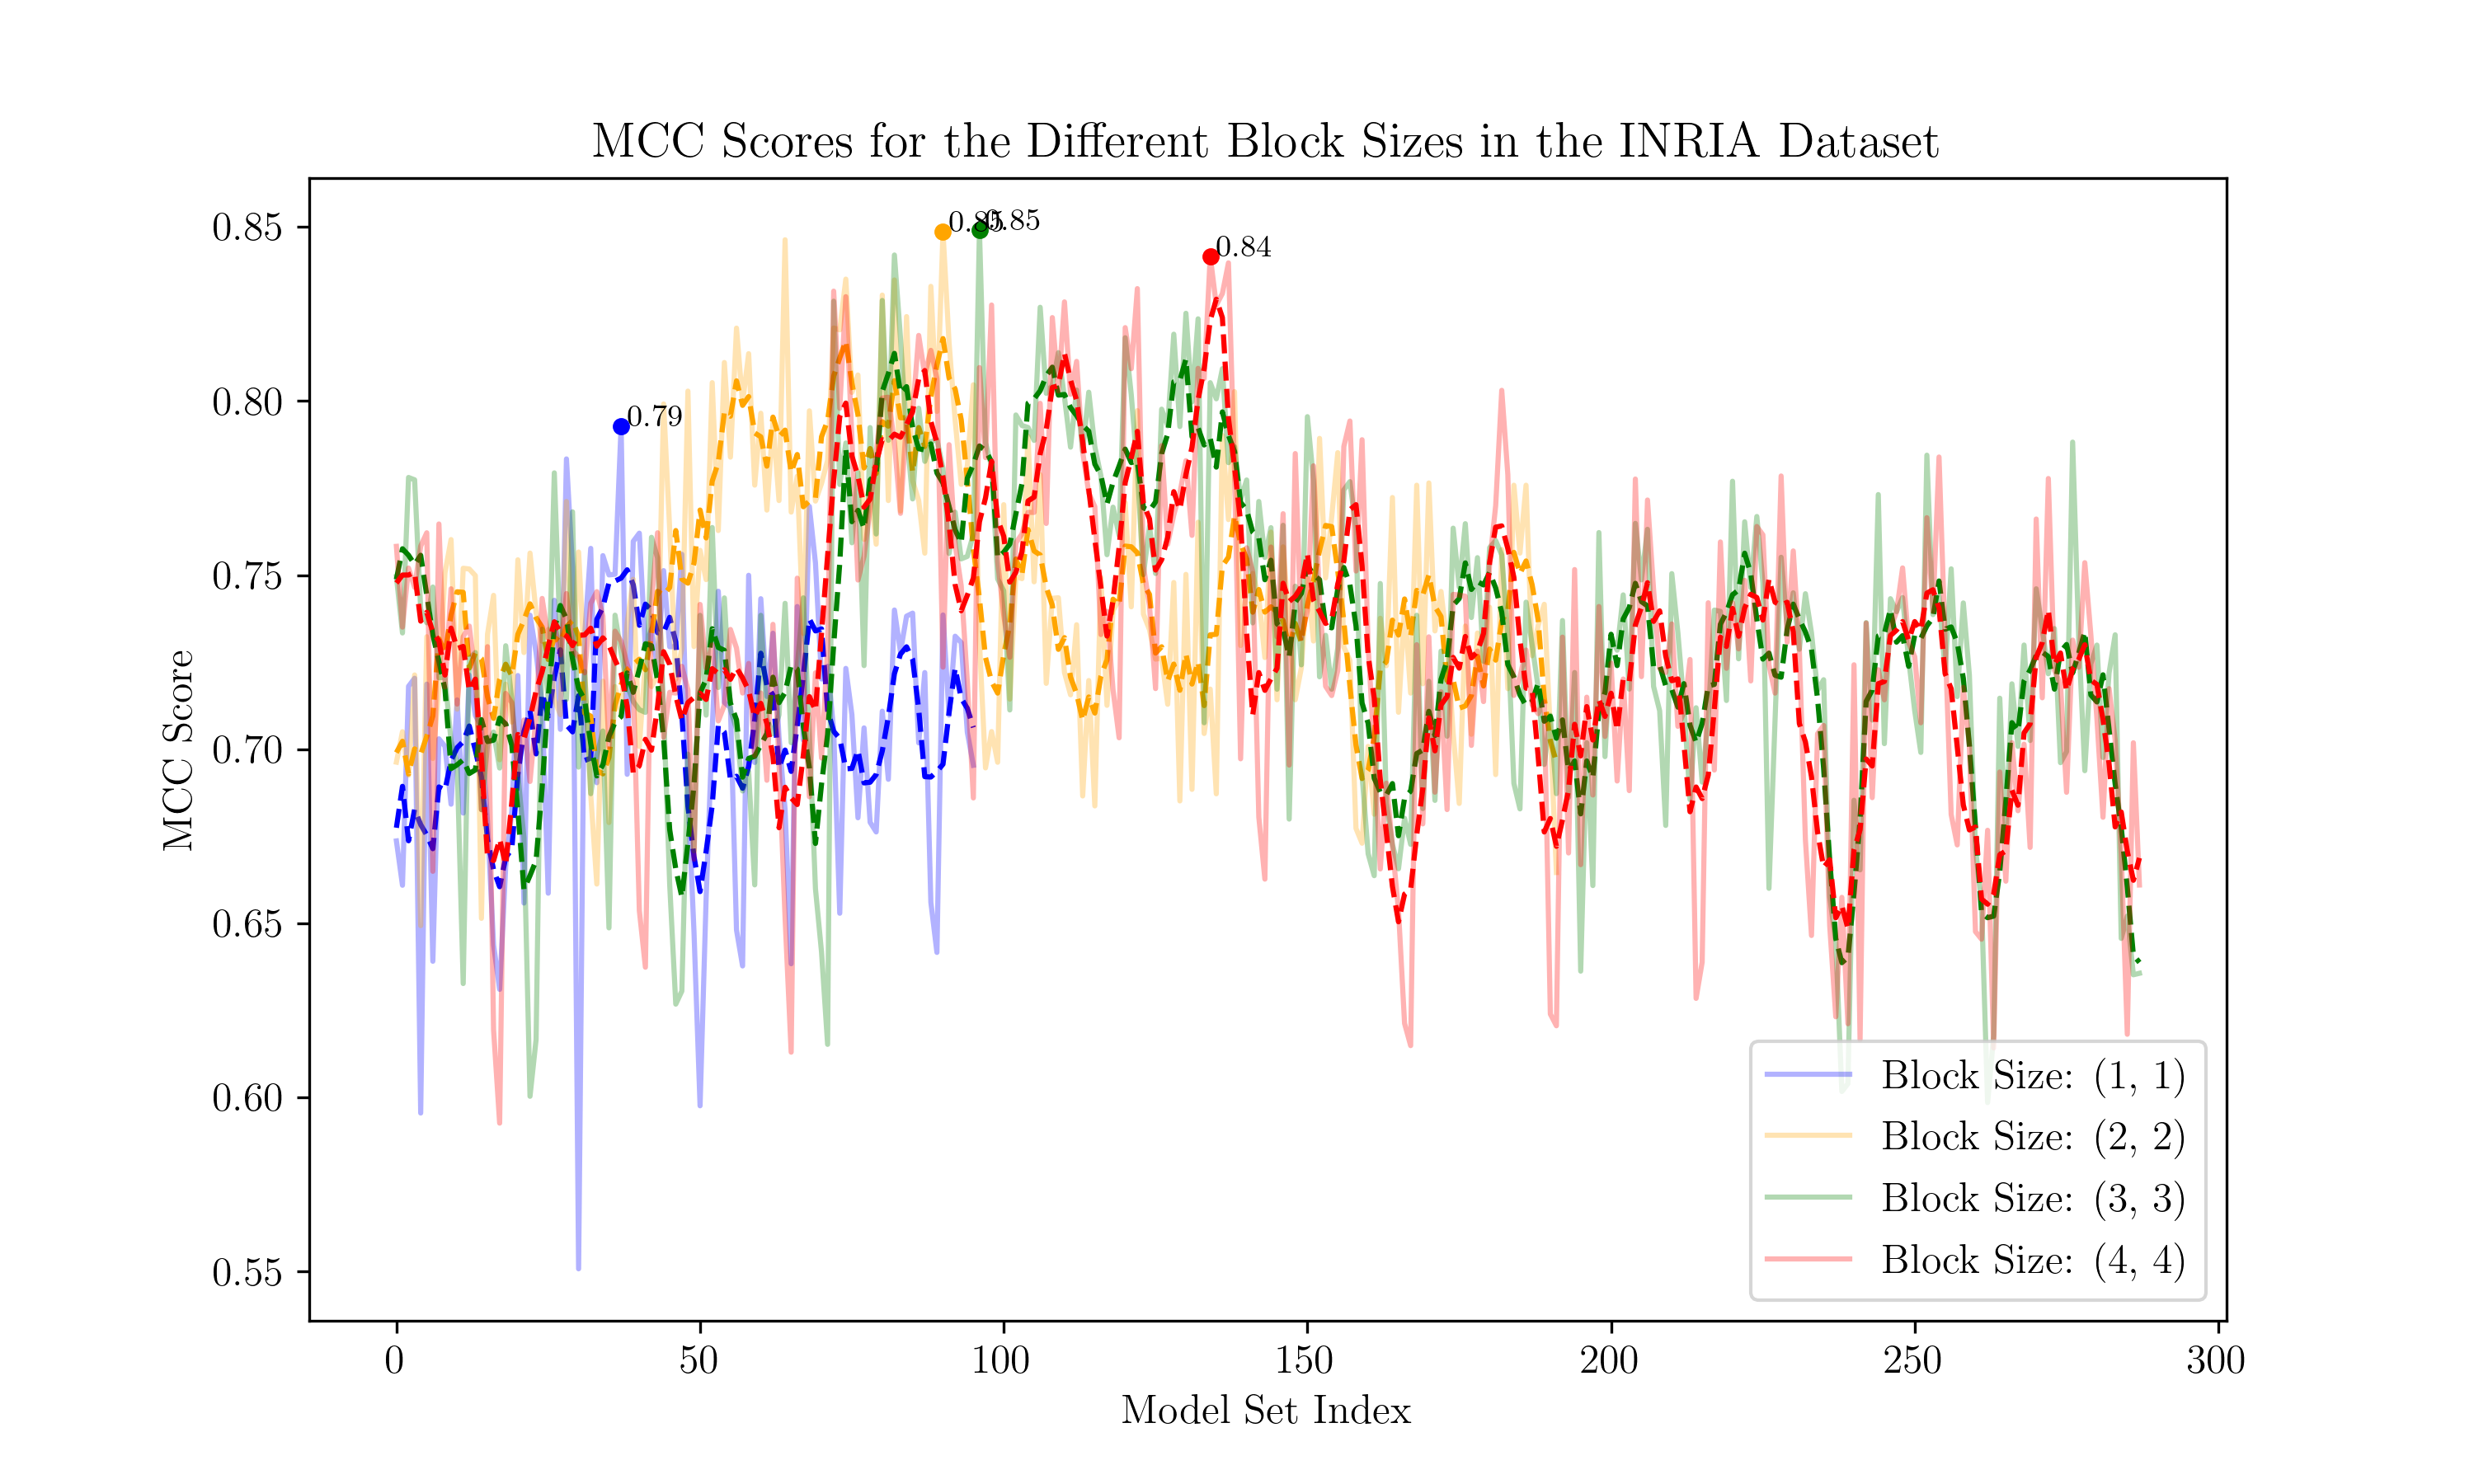
\includegraphics[width=0.9\linewidth]{mcc_block_size_INRIA.png}
    \caption{
        MCC scores for INRIA dataset, grouped by block size.
    }
\end{figure}

\begin{figure}
    \centering
    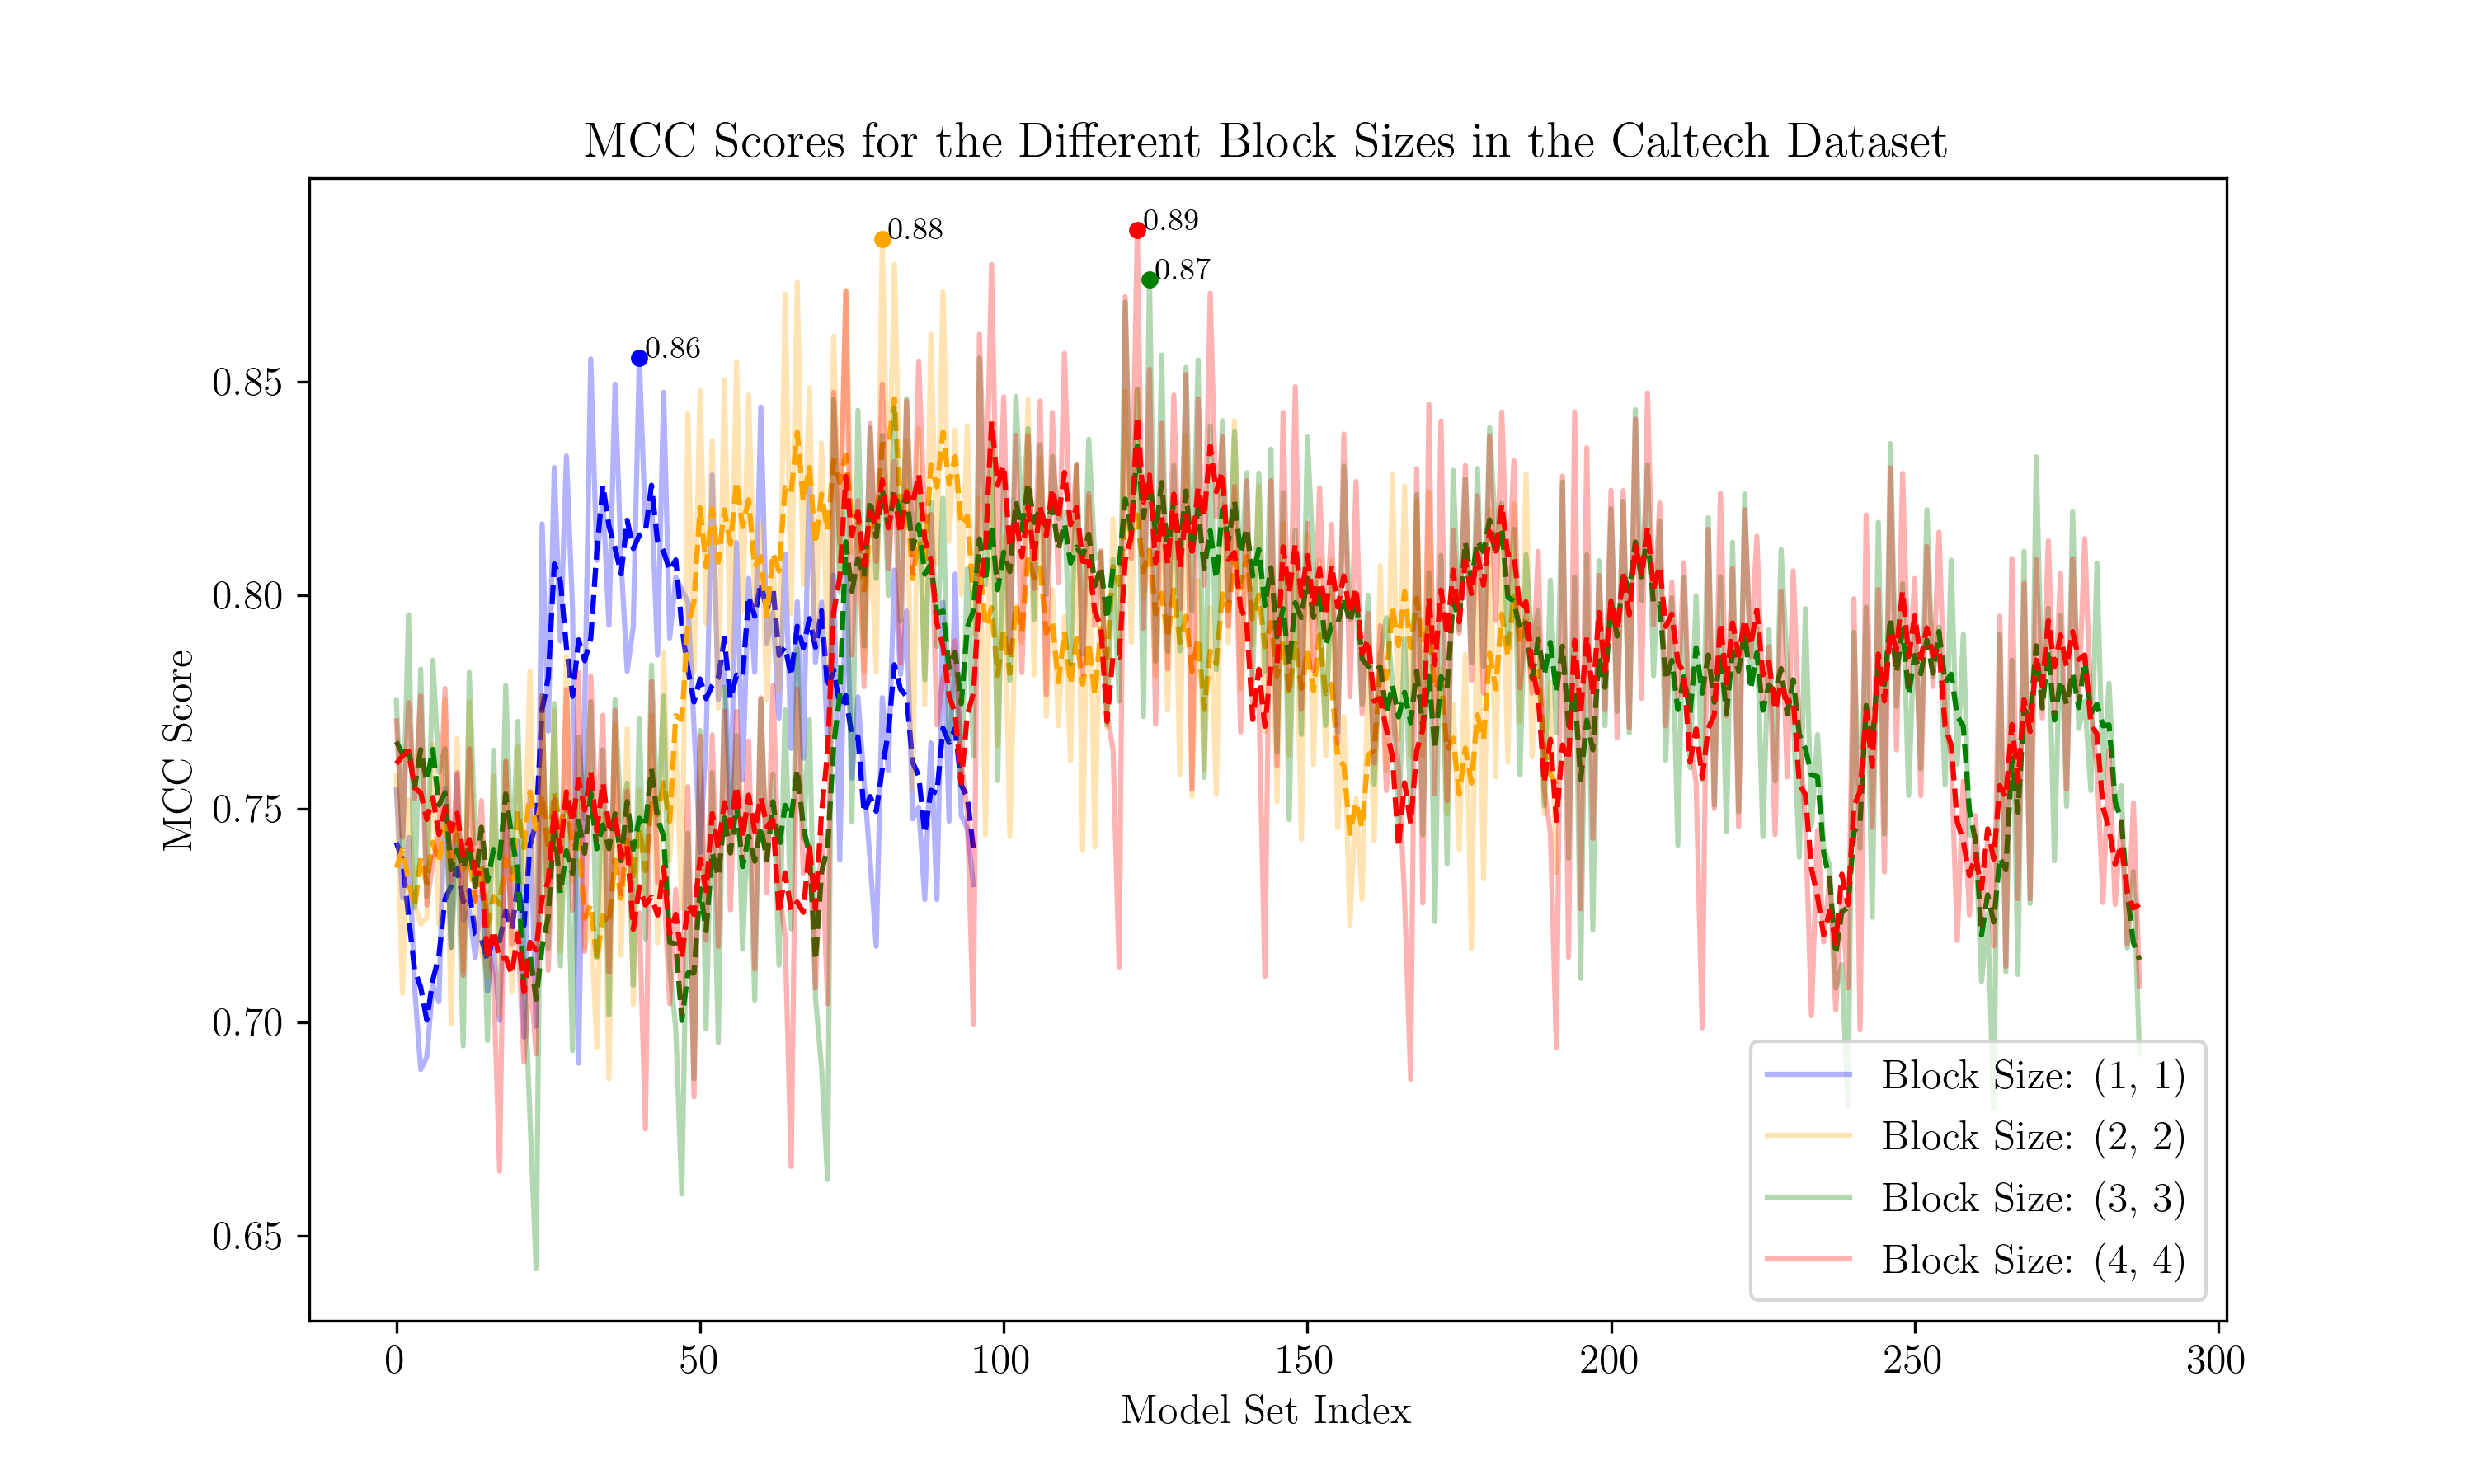
\includegraphics[width=0.9\linewidth]{mcc_block_size_caltech_30.png}
    \caption{
        MCC scores for Caltech dataset, grouped by block size.
    }
\end{figure}

\begin{figure}
    \centering
    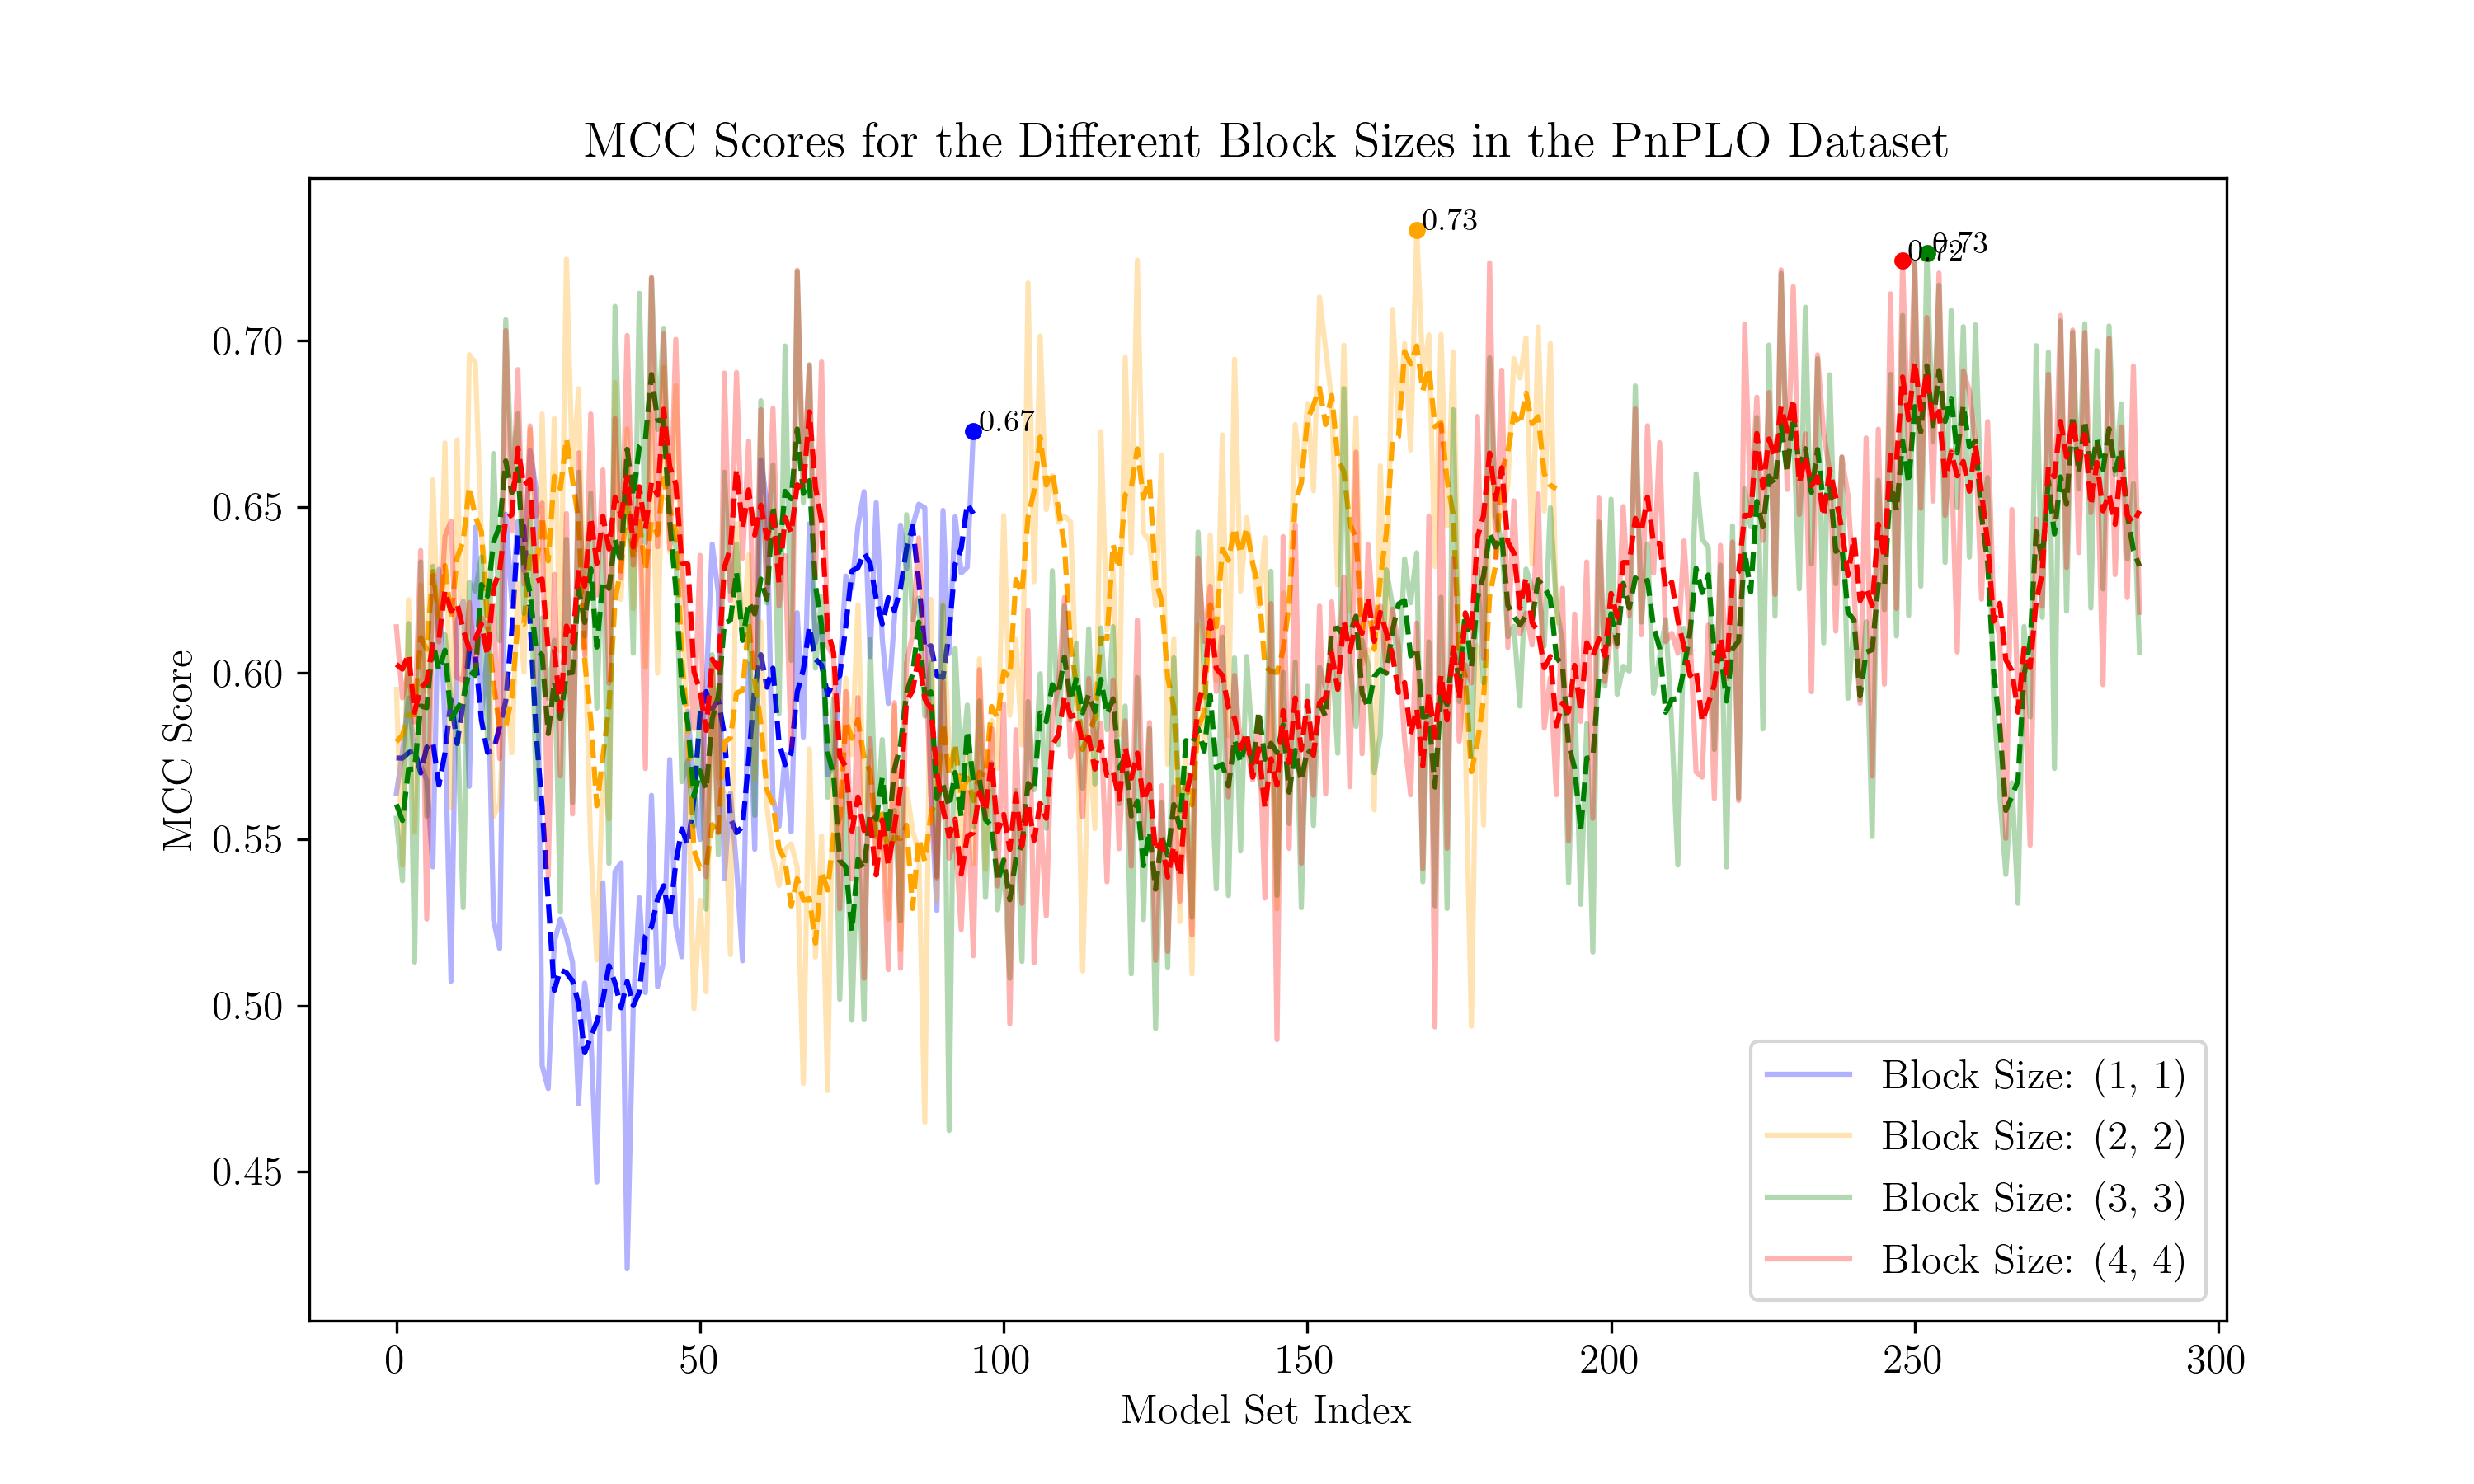
\includegraphics[width=0.9\linewidth]{mcc_block_size_PnPLO.png}
    \caption{
        MCC scores for PnPLO dataset, grouped by block size.
    }
\end{figure}

\begin{figure}
    \centering
    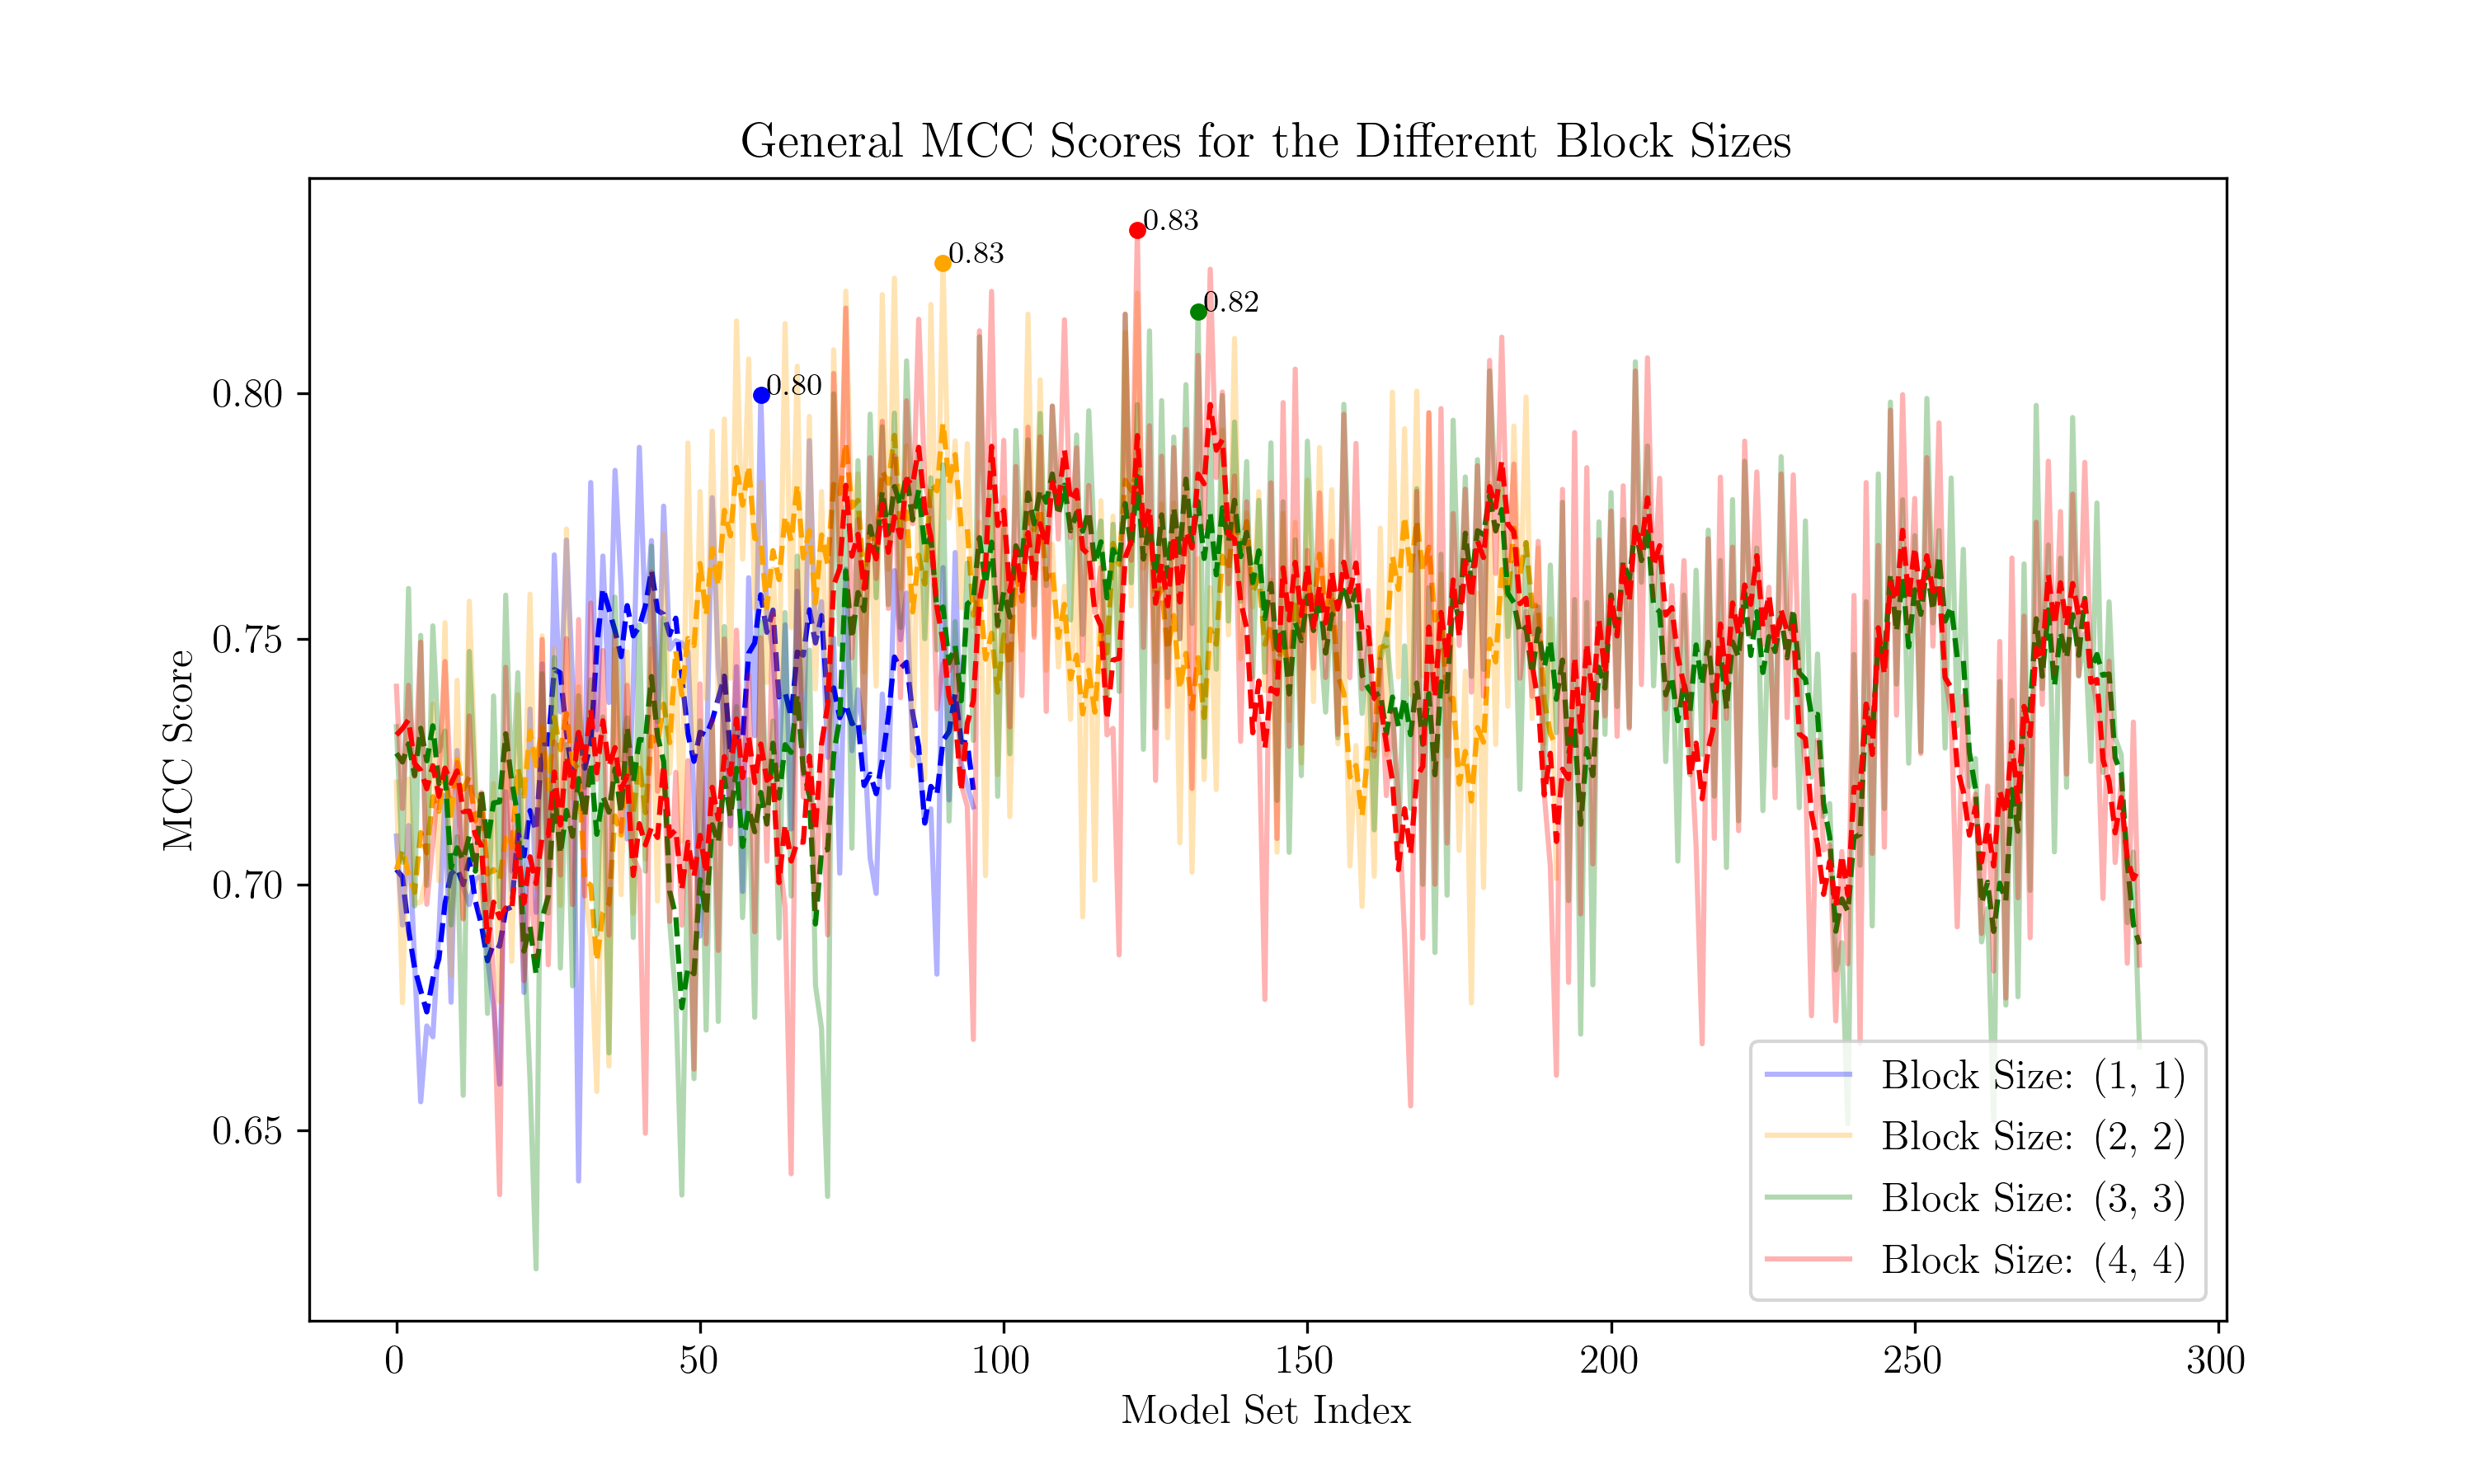
\includegraphics[width=0.9\linewidth]{mcc_block_size_total.png}
    \caption{
        MCC scores for the aggregate test dataset, grouped by block size.
    }
\end{figure}

\subsubsection{Graphs for Block Sizes with Different Block Strides}

\begin{figure}
    \centering
    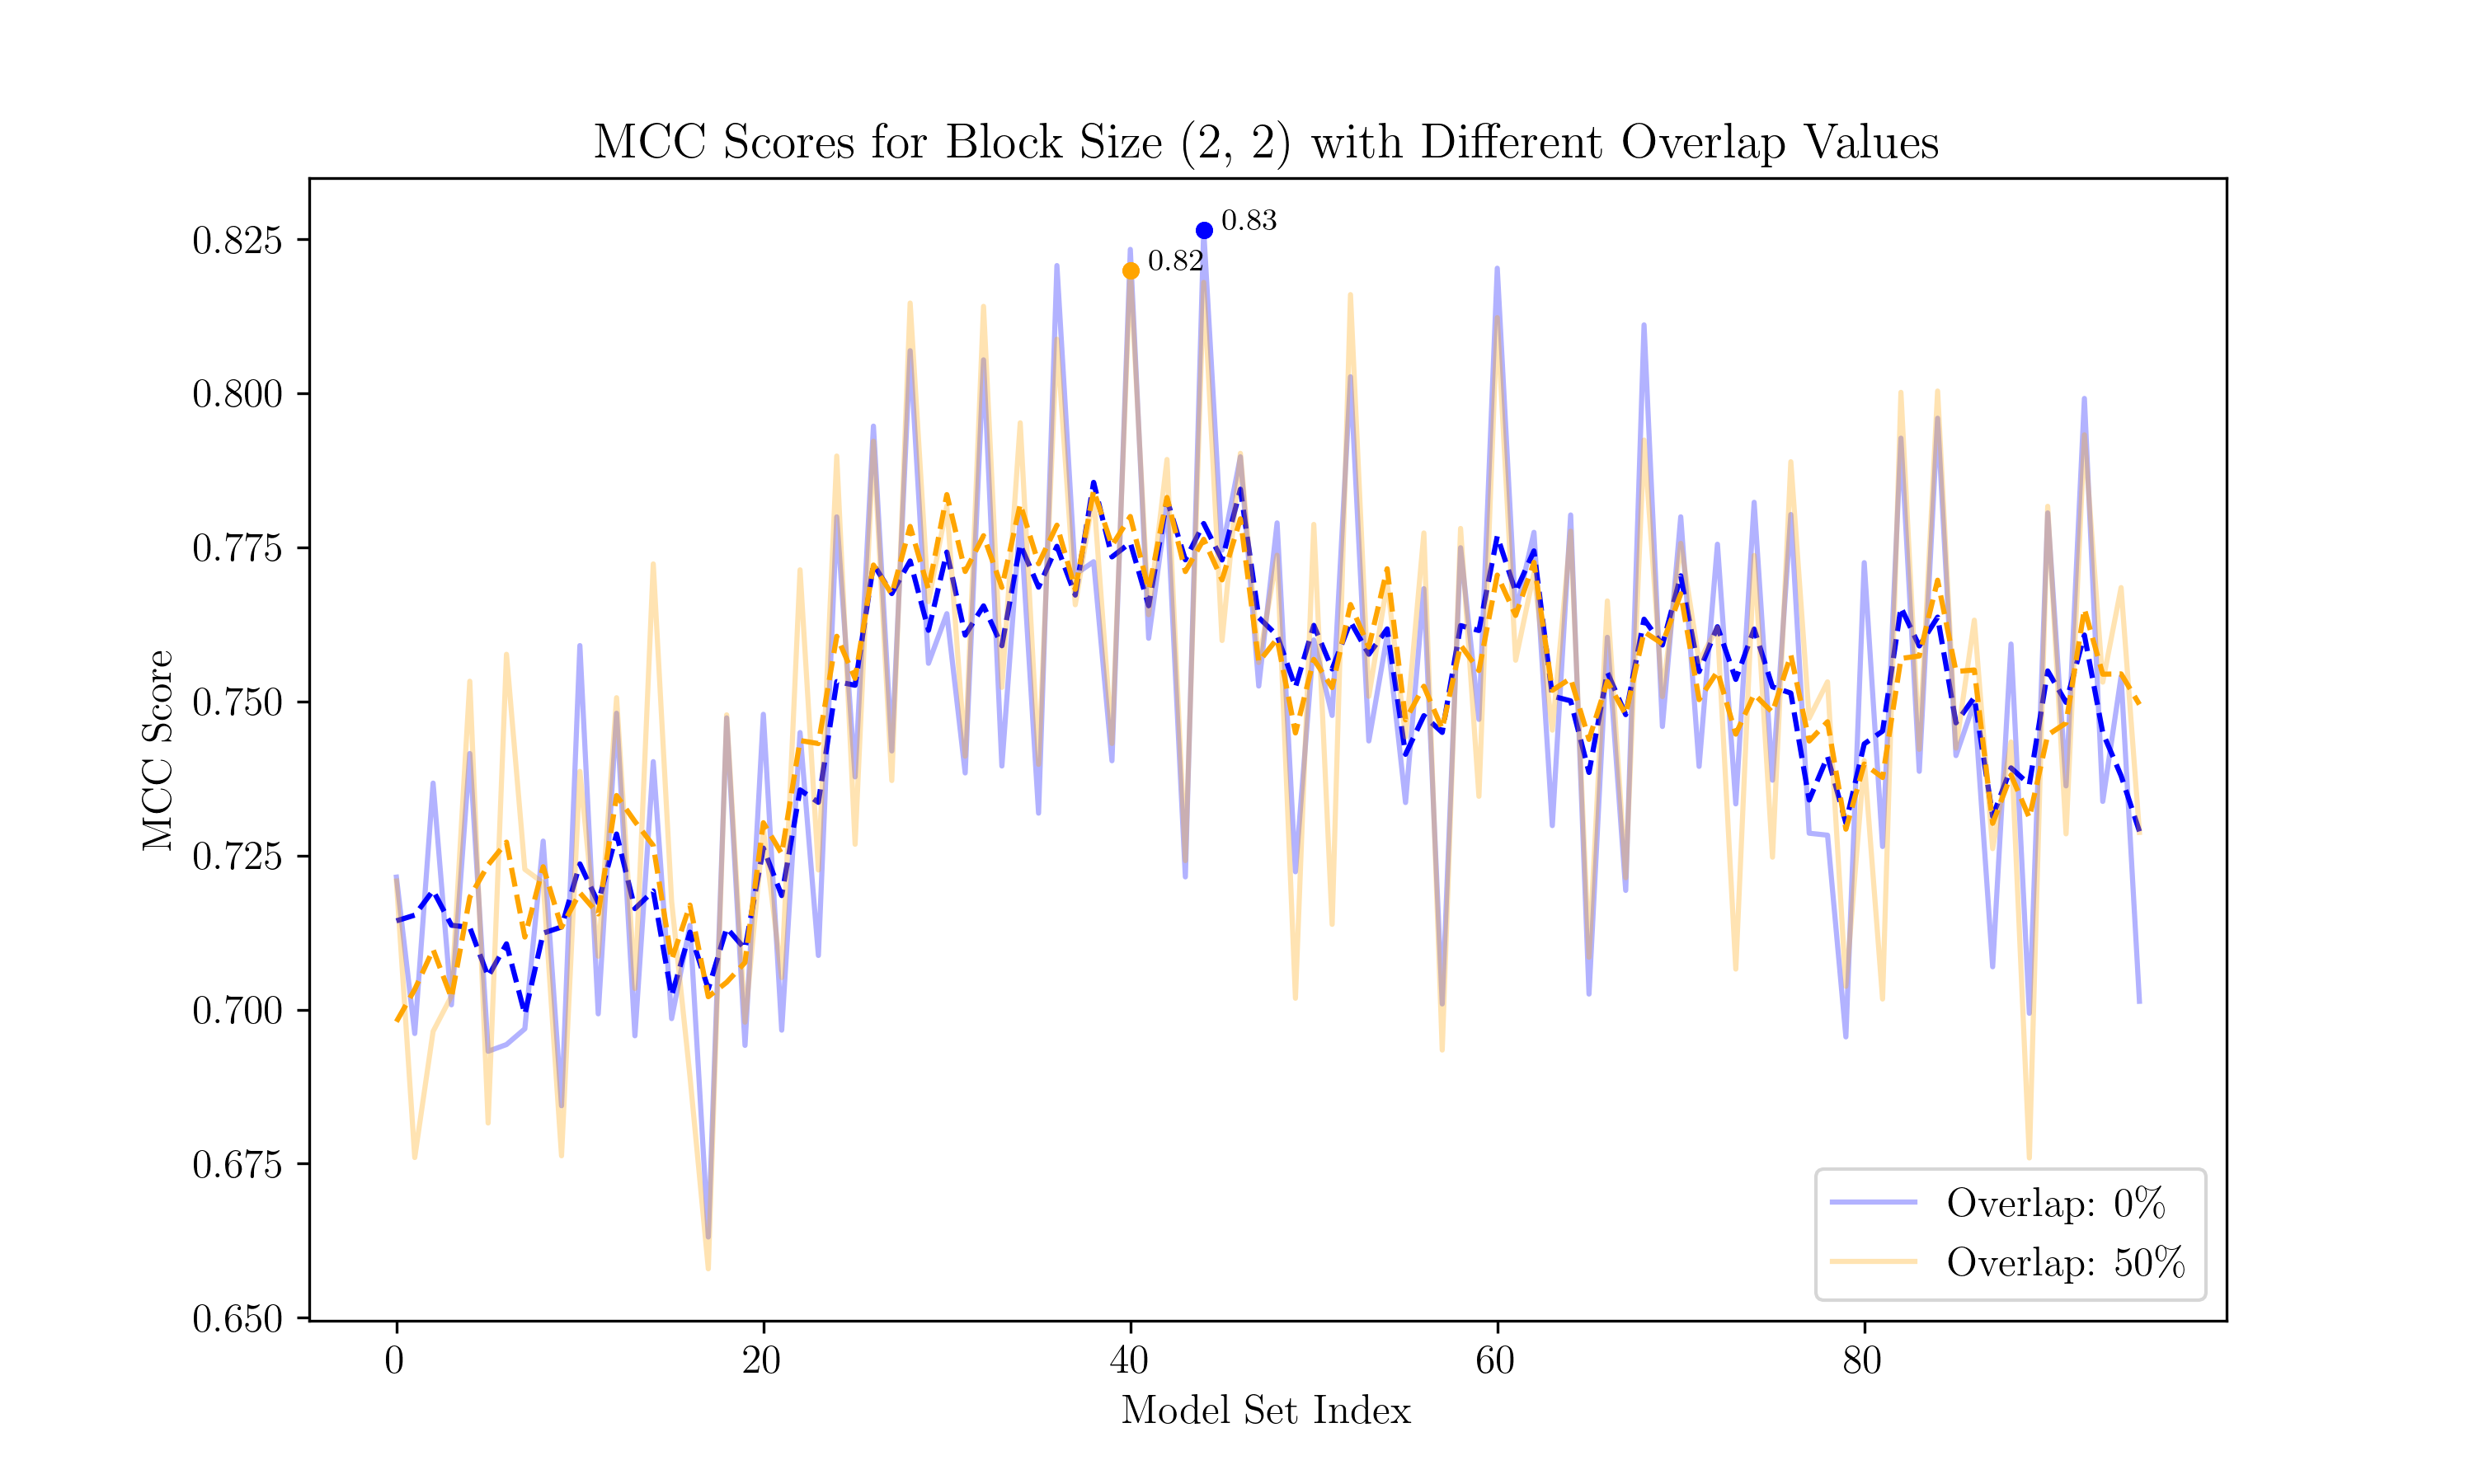
\includegraphics[width=0.9\linewidth]{mcc_overlap_(2, 2).png}
    \caption{
        MCC scores for the aggregate test dataset, grouped by block size and block stride. The block stride is set to (2, 2). The overlap is defined by $1 - \frac{\text{block stride (h or w)}}{\text{block size (h or w)}}$ since the horizontal and vertical components of both block stride values and block sizes values are respectively identical.
    }
\end{figure}

\begin{figure}
    \centering
    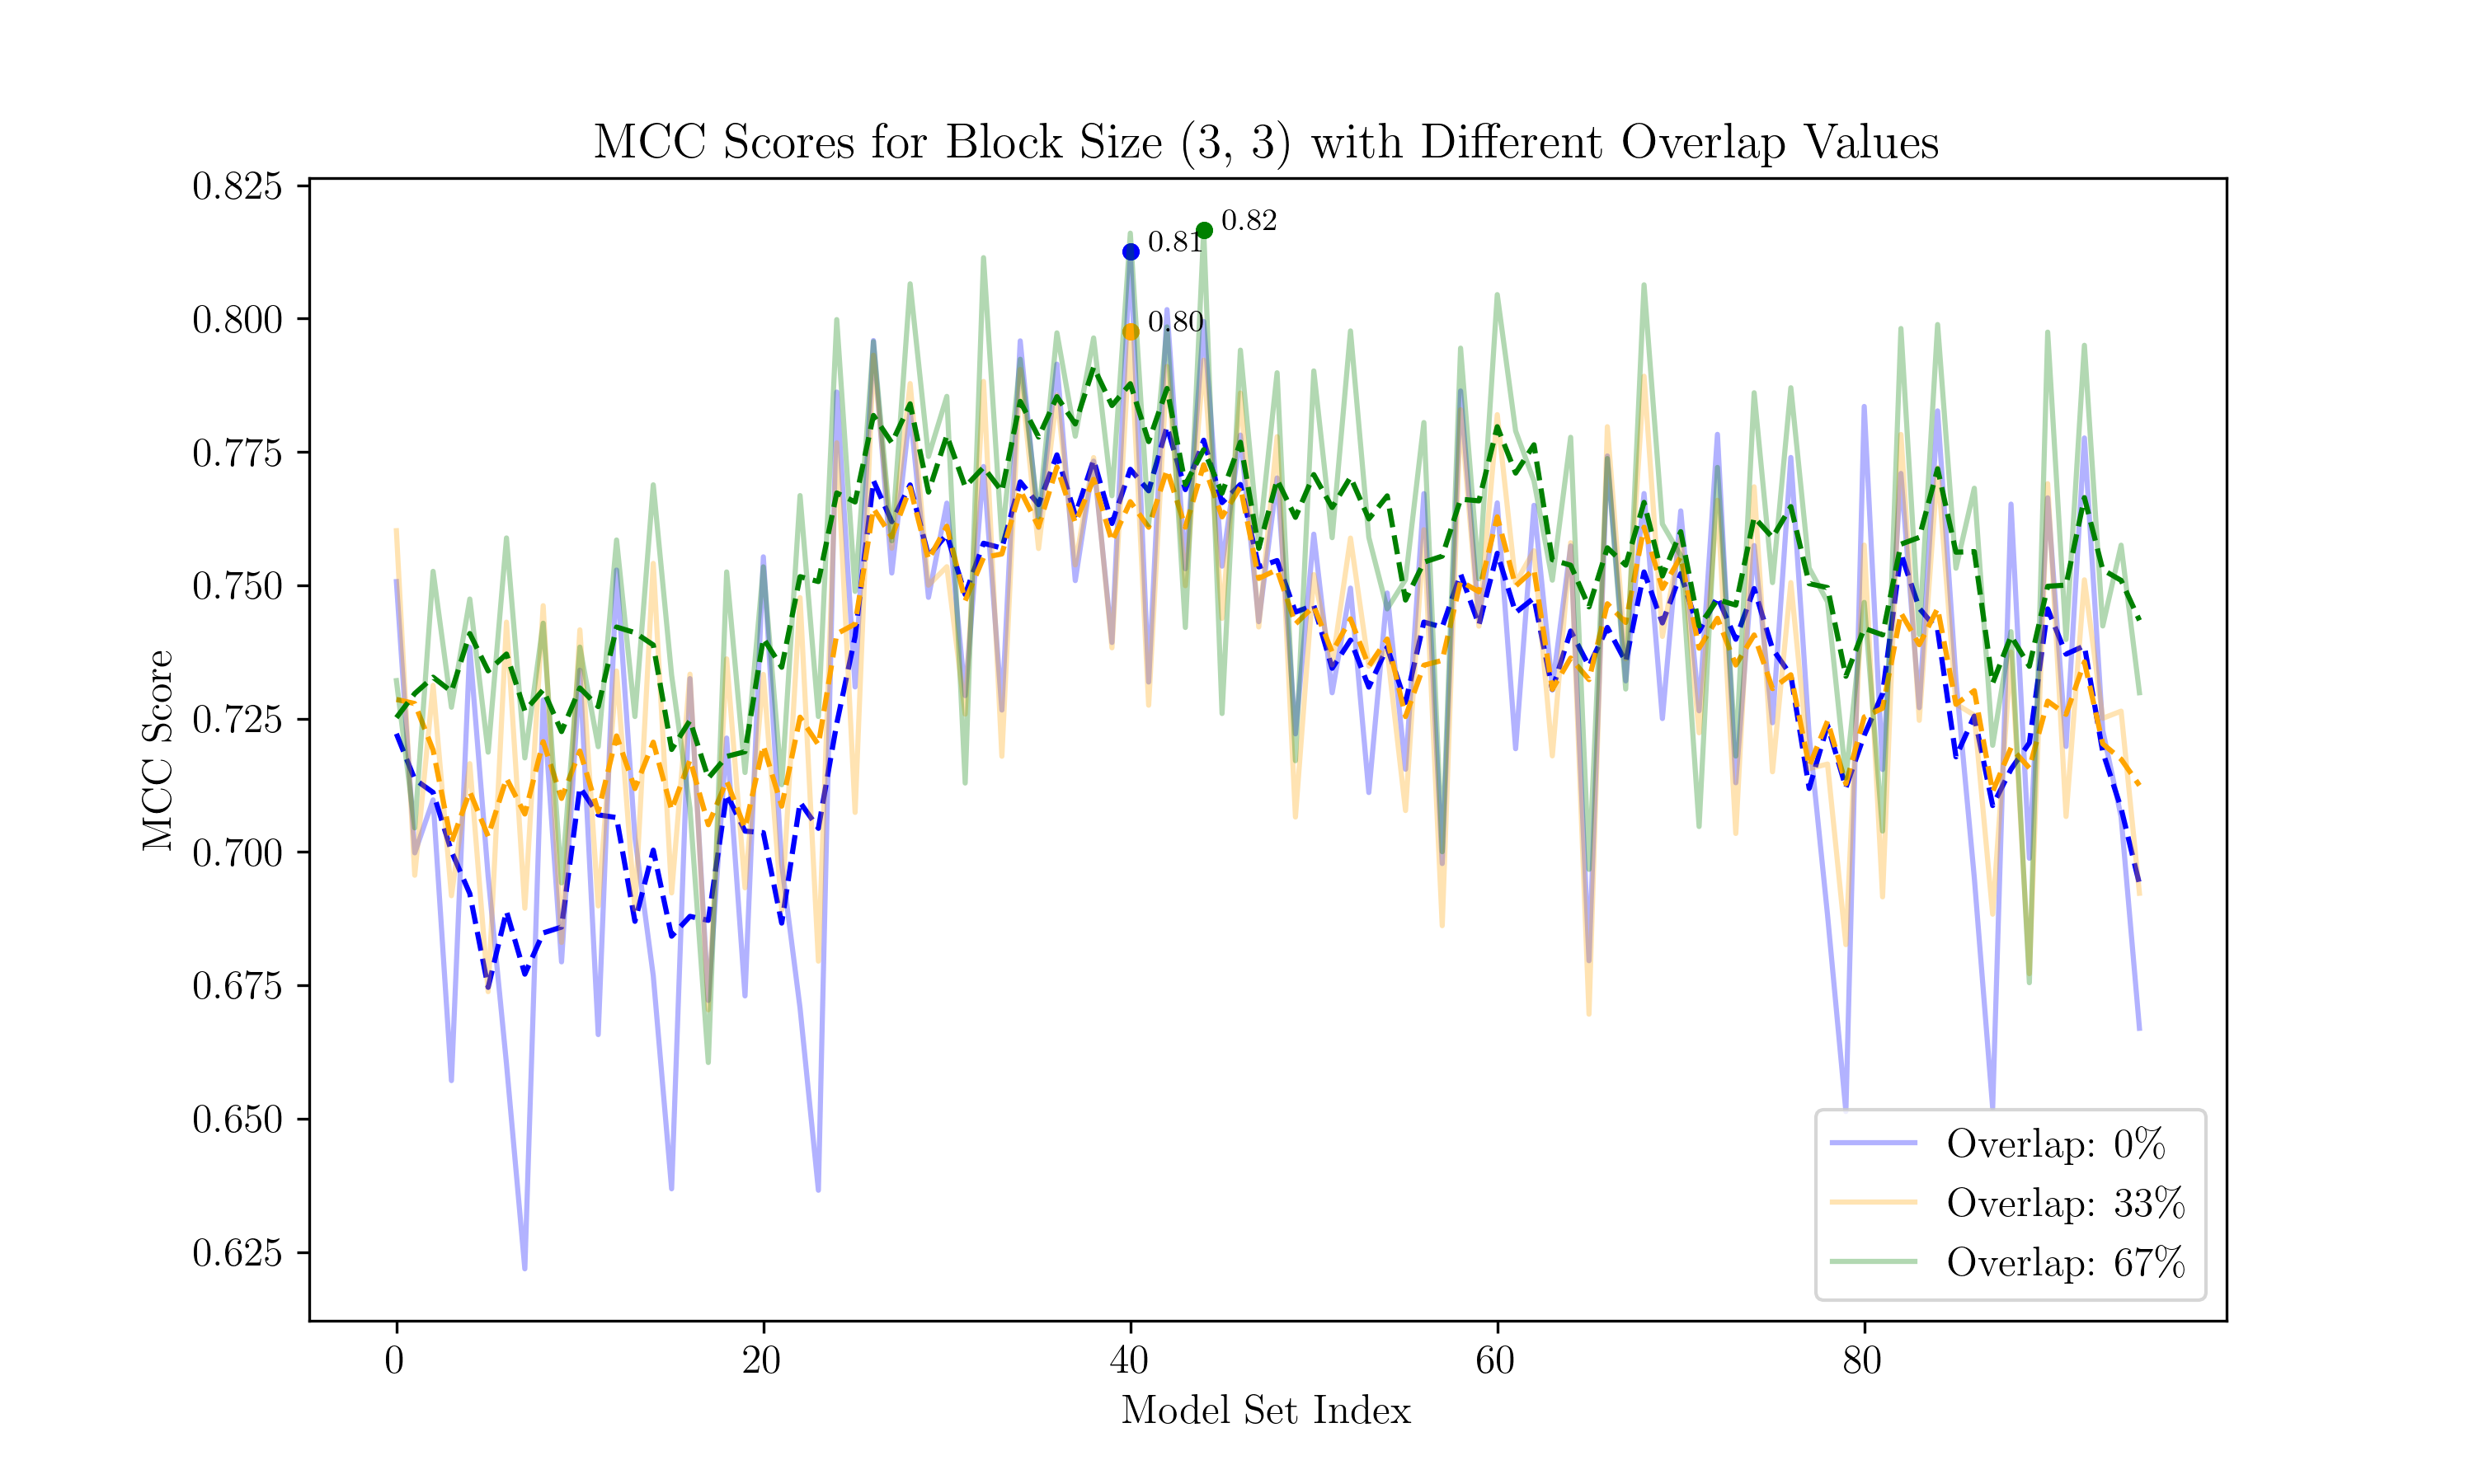
\includegraphics[width=0.9\linewidth]{mcc_overlap_(3, 3).png}
    \caption{
        MCC scores for the aggregate test dataset, grouped by block size and block stride. The block stride is set to (3, 3). The overlap is defined by $1 - \frac{\text{block stride (h or w)}}{\text{block size (h or w)}}$ since the horizontal and vertical components of both block stride values and block sizes values are respectively identical.
    }
\end{figure}

\begin{figure}
    \centering
    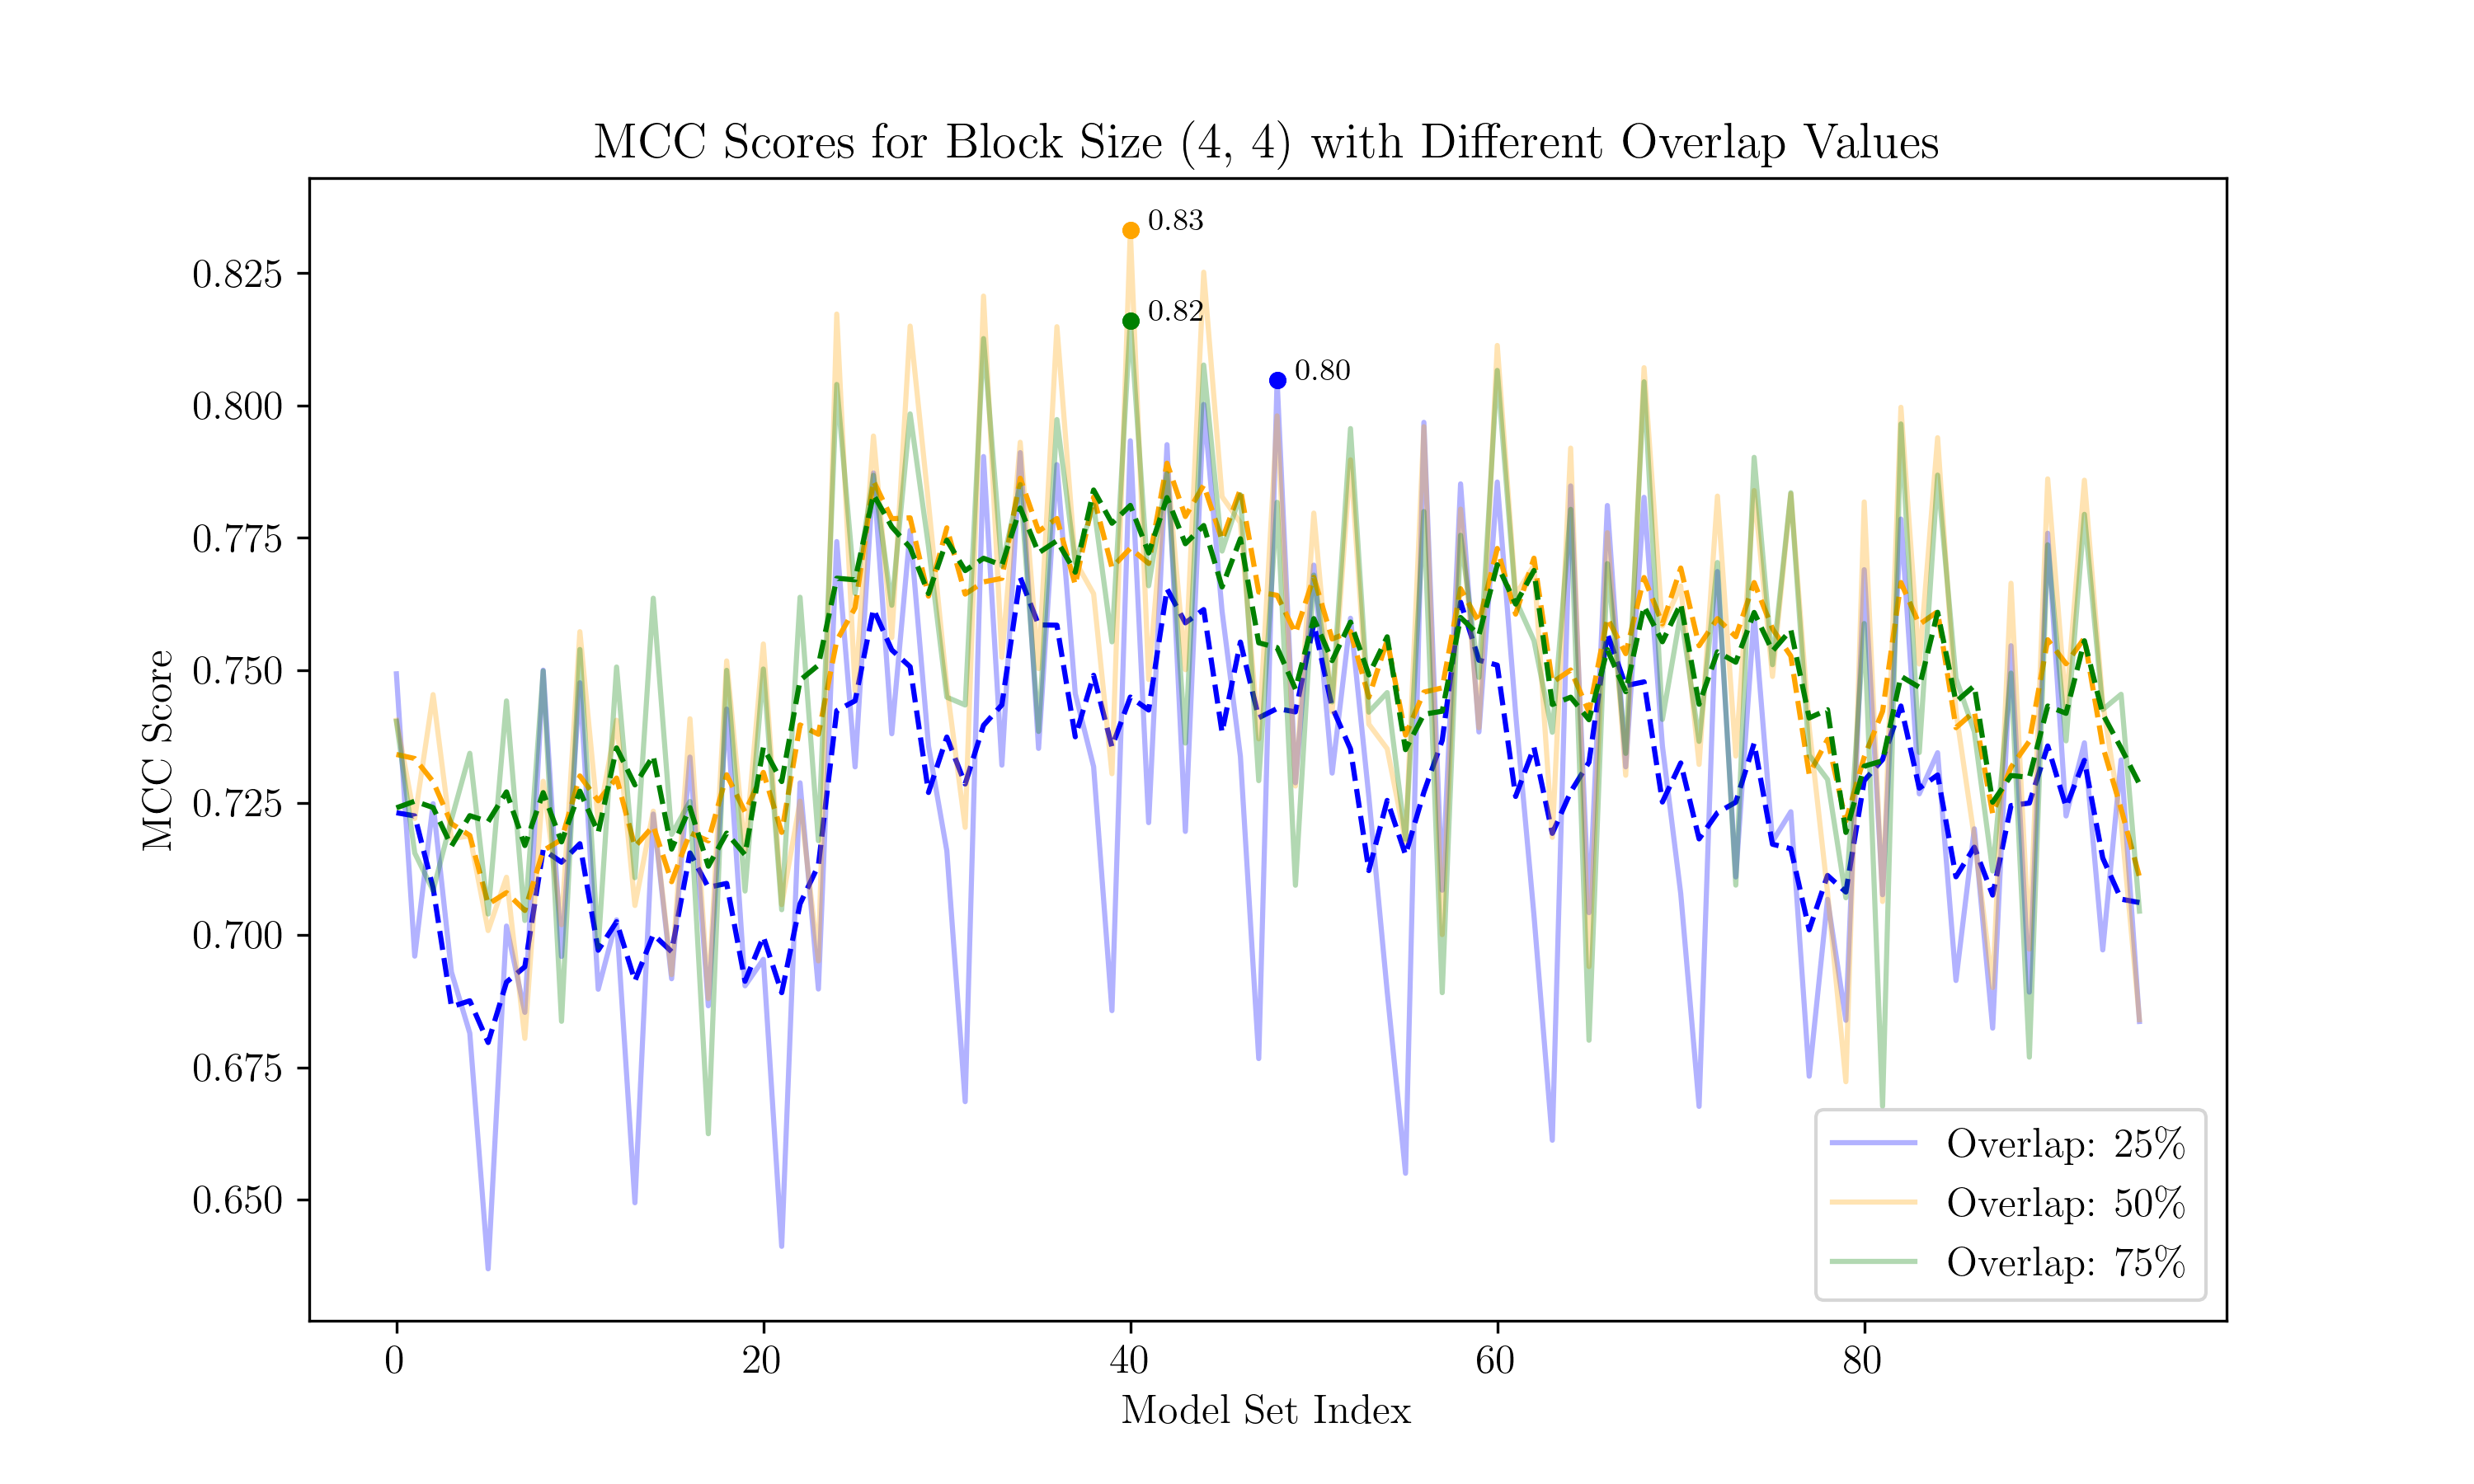
\includegraphics[width=0.9\linewidth]{mcc_overlap_(4, 4).png}
    \caption{
        MCC scores for the aggregate test dataset, grouped by block size and block stride. The block stride is set to (4, 4). The overlap is defined by $1 - \frac{\text{block stride (h or w)}}{\text{block size (h or w)}}$ since the horizontal and vertical components of both block stride values and block sizes values are respectively identical.
    }
\end{figure}